% \documentclass[10pt,journal,compsoc]{IEEEtran}
% \documentclass[lettersize,journal]{IEEEtran}
\documentclass[journal]{IEEEtran}

\usepackage{array}
\usepackage[caption=false,font=normalsize,labelfont=sf,textfont=sf]{subfig}
\usepackage{textcomp}
\usepackage{stfloats}
\usepackage{url}
\usepackage{verbatim}
\usepackage{graphicx}
\usepackage{cite}

\usepackage{algorithmic}
\usepackage{algorithm}
\usepackage{amsmath,amsfonts}
\usepackage{mathrsfs}
\usepackage{booktabs}
\usepackage{multirow}


\newtheorem{theorem}{Theorem}%[section]
\newtheorem{proposition}{Proposition}
\newtheorem{lemma}{Lemma}
\newtheorem{definition}{Definition}
\newtheorem{assumption}{Assumption}



% *** CITATION PACKAGES ***
%
\ifCLASSOPTIONcompsoc
  % IEEE Computer Society needs nocompress option
  % requires cite.sty v4.0 or later (November 2003)
  \usepackage[nocompress]{cite}
\else
  % normal IEEE
  \usepackage{cite}
\fi


% *** GRAPHICS RELATED PACKAGES ***
%
\ifCLASSINFOpdf
%   \usepackage[pdftex]{graphicx}
  % declare the path(s) where your graphic files are
  % \graphicspath{{../pdf/}{../jpeg/}}
  % and their extensions so you won't have to specify these with
  % every instance of \includegraphics
  % \DeclareGraphicsExtensions{.pdf,.jpeg,.png}
\else
  % or other class option (dvipsone, dvipdf, if not using dvips). graphicx
  % will default to the driver specified in the system graphics.cfg if no
  % driver is specified.
  % \usepackage[dvips]{graphicx}
  % declare the path(s) where your graphic files are
  % \graphicspath{{../eps/}}
  % and their extensions so you won't have to specify these with
  % every instance of \includegraphics
  % \DeclareGraphicsExtensions{.eps}
\fi
% graphicx was written by David Carlisle and Sebastian Rahtz. It is
% required if you want graphics, photos, etc. graphicx.sty is already
% installed on most LaTeX systems. The latest version and documentation
% can be obtained at: 
% http://www.ctan.org/pkg/graphicx
% Another good source of documentation is "Using Imported Graphics in
% LaTeX2e" by Keith Reckdahl which can be found at:
% http://www.ctan.org/pkg/epslatex
%
% latex, and pdflatex in dvi mode, support graphics in encapsulated
% postscript (.eps) format. pdflatex in pdf mode supports graphics
% in .pdf, .jpeg, .png and .mps (metapost) formats. Users should ensure
% that all non-photo figures use a vector format (.eps, .pdf, .mps) and
% not a bitmapped formats (.jpeg, .png). The IEEE frowns on bitmapped formats
% which can result in "jaggedy"/blurry rendering of lines and letters as
% well as large increases in file sizes.
%
% You can find documentation about the pdfTeX application at:
% http://www.tug.org/applications/pdftex




% correct bad hyphenation here
% \hyphenation{op-tical net-works semi-conduc-tor}
\hyphenation{op-tical net-works semi-conduc-tor IEEE-Xplore}

\begin{document}
% \title{Wasserstein Distributionally Robust Domain Generalization  with Adaptive Inference}
% \title{Wasserstein Distributionally Robust % Domain Generalization} 
% \title{Wasserstein Distributionally Robust Optimization for Domain Generalization} 
% \title{Learning Generalizable Models via Wasserstein Distributionally Robust Optimization} 
% \title{To Generalize to New Domains via Wasserstein Distributionally Robust Optimization} 
\title{Generalizing to Unseen Domains with Wasserstein Distributional Robustness under Limited Source Knowledge} 
\author{Jingge Wang, Liyan Xie, Yao Xie, Shao-Lun Huang and Yang Li % <-this % stops a space
\IEEEcompsocitemizethanks{
\IEEEcompsocthanksitem Jingge Wang, Shao-Lun Huang and Yang Li are with Tsinghua-Berkeley Shenzhen Institute, Tsinghua University, China.%\protect\\
% E-mail: wjg22@mails.tsinghua.edu.cn; shaolun.huang@sz.tsinghua.edu.cn; yangli@sz.tsinghua.edu.cn.
\IEEEcompsocthanksitem Liyan Xie is with the School of Data Science, The Chinese University of Hong Kong, Shenzhen.%\protect\\
% E-mail: xieliyan@cuhk.edu.cn.
\IEEEcompsocthanksitem Yao Xie is with the School of Industrial and Systems and Engineering, Georgia Institute of Technology.%\protect\\
% E-mail: yao.xie@isye.gatech.edu.
}
% \thanks{Manuscript received xx xx, xx; revised xx xx, xx.}
}



% % The paper headers
% \markboth{Journal of \LaTeX\ Class Files,~Vol.~18, No.~9, September~2020}
% % \markboth{Journal of \LaTeX\ Class Files,~Vol.~XX, No.~XX, XX~XX}%
% % {Shell \MakeLowercase{\textit{et al.}}: Bare Demo of IEEEtran.cls for Computer Society Journals}
% The paper headers
\markboth{Journal of \LaTeX\ Class Files,~Vol.~14, No.~8, August~2021}%
{Shell \MakeLowercase{\textit{et al.}}: A Sample Article Using IEEEtran.cls for IEEE Journals}
\IEEEpubid{0000--0000/00\$00.00~\copyright~2021 IEEE}
% Remember, if you use this you must call \IEEEpubidadjcol in the second
% column for its text to clear the IEEEpubid mark.

\maketitle
% \IEEEtitleabstractindextext{
\begin{abstract}
Domain generalization aims at learning a universal model that performs well on unseen target domains, incorporating knowledge from multiple source domains.
In this research, we consider the scenario where different domain shifts occur among conditional distributions of different classes across domains.
When labeled samples in the source domains are limited, existing approaches are not sufficiently robust. 
To address this problem, 
we propose a novel domain generalization framework called {Wasserstein Distributionally Robust Domain Generalization} (WDRDG),
inspired by the concept of distributionally robust
optimization. We encourage robustness over conditional distributions within class-specific Wasserstein uncertainty sets and optimize the worst-case performance of a classifier over
these uncertainty sets.
We further develop a test-time adaptation module leveraging optimal transport to quantify the relationship between the unseen target domain and source domains to make adaptive inference for target data.
Experiments on the Rotated MNIST, PACS and the VLCS datasets demonstrate that our method could effectively balance the robustness and discriminability in challenging generalization scenarios.
\end{abstract}


% Note that keywords are not normally used for peerreview papers.
\begin{IEEEkeywords}
Domain generalization, distributionally robust optimization, optimal transport, Wasserstein uncertainty set.
\end{IEEEkeywords}
% }


% \maketitle

% To allow for easy dual compilation without having to reenter the
% abstract/keywords data, the \IEEEtitleabstractindextext text will
% not be used in maketitle, but will appear (i.e., to be "transported")
% here as \IEEEdisplaynontitleabstractindextext when the compsoc 
% or transmag modes are not selected <OR> if conference mode is selected 
% - because all conference papers position the abstract like regular
% papers do.

% \IEEEdisplaynontitleabstractindextext
% \IEEEdisplaynontitleabstractindextext has no effect when using
% compsoc or transmag under a non-conference mode.



% For peer review papers, you can put extra information on the cover
% page as needed:
% \ifCLASSOPTIONpeerreview
% \begin{center} \bfseries EDICS Category: 3-BBND \end{center}
% \fi
%
% For peerreview papers, this IEEEtran command inserts a page break and
% creates the second title. It will be ignored for other modes.

% \IEEEpeerreviewmaketitle



\section{Introduction}
% \IEEEraisesectionheading{\section{Introduction}\label{sec:introduction}}
% Computer Society journal (but not conference!) papers do something unusual
% with the very first section heading (almost always called "Introduction").
% They place it ABOVE the main text! IEEEtran.cls does not automatically do
% this for you, but you can achieve this effect with the provided
% \IEEEraisesectionheading{} command. Note the need to keep any \label that
% is to refer to the section immediately after \section in the above as
% \IEEEraisesectionheading puts \section within a raised box.




% The very first letter is a 2 line initial drop letter followed
% by the rest of the first word in caps (small caps for compsoc).
% 
% form to use if the first word consists of a single letter:
% \IEEEPARstart{A}{demo} file is ....
% 
% form to use if you need the single drop letter followed by
% normal text (unknown if ever used by the IEEE):
% \IEEEPARstart{A}{}demo file is ....
% 
% Some journals put the first two words in caps:
% \IEEEPARstart{T}{his demo} file is ....
% 
% Here we have the typical use of a "T" for an initial drop letter
% and "HIS" in caps to complete the first word.
\IEEEPARstart{I}{n} many practical learning applications, labeled training data are only available from fragmented source domains. It is thus a challenge to learn a robust model for future data that could come from a new domain, with unknown domain shift. One commonly acknowledged solution to this challenge is domain generalization \cite{blanchard2011generalizing}, which aims at learning a model that generalizes well to target domains based on available training data from multiple source domains and in a total absence of prior knowledge about the target domain. A surge of popularity has been seen recently in the application of domain generalization in various fields, such as computer vision \cite{gong2019dlow,shi2020towards,zhou2020learning,zhou2021learning,yue2019domain,volpi2018generalizing,shao2019multi}, natural processing \cite{balaji2018metareg,marzinotto2019robust,stepanov2014towards,fried2019cross}, and reinforcement learning \cite{li2018learning}, etc.


% 1. not at all considering possible target shift 
% Numerous efficient methods have been developed for generalization to the target domain when source data from the source domains are available to be exploited in learning a robust model.
Numerous methods have been developed for learning a generalizable model by exploiting the available data from the source domains,
where the shifts across these source domains are implicitly assumed to be representative of the target shift that we will meet at test time. 
% examples of such methods 
% representation learning based DG 
The well-known approaches include learning domain-invariant feature representations through kernel functions \cite{blanchard2011generalizing,muandet2013domain,ghifary2016scatter,blanchard2017domain,grubinger2015domain,li2018domain2,hu2020domain}, or by distribution alignment \cite{zhou2020domain,peng2019moment,motiian2017unified}, or in an adversarial manner \cite{li2018domain,Gong_2019_CVPR,li2018deep,shao2019multi,rahman2020correlation}.
The learned invariance across source domains, however, may not be typical if the unseen target shift is of extreme magnitude.
% source training samples are limited. 
In this case, forcing distributions to align in a common representation space may result in a biased model that overfits the source domains,
and only performs well for target domains that are similar to certain source domains.
% Forcing distributions to align in a common representation space relies on the diversity and quantity of the source data and would easily overfit the limited training data, resulting in a conservative model that may only perform well for target domains similar to source domains.
% learning strategy ensemble learning based DG
% Some ensemble learning-based domain generalization methods \cite{mancini2018best, segu2020batch} assign larger weights to more related source domains at test time to fuse multiple domain-specific models. The main drawback is 
% they demand the richness of source domain shifts to  represent the possible target shifts, and also sufficient source knowledge to ensure the reliability of each source model.
% % reliability of source models and the estimation of relevance all rely on the sufficiency of source data. 
% % In order to gather the power of domain-specific models for each source domain, the predictions from multiple source models could be aggregated by assigning larger weights to more related source domains in ensemble learning-based methods \cite{mancini2018best, segu2020batch}. 
% % However, when the source domains contain only insufficient labeled data, the estimation of relevance would be inaccurate.

% 2. Explicitly simulate possible target domain shift 
% However, implicitly assuming the shifts across source domains to be representative of possible target shifts may limit the robustness of a learned model to extreme target shifts. 
Instead, to explicitly model unseen target domain shifts, meta-learning-based domain generalization methods like MLDG \cite{li2018learning}
% , MetaReg \cite{balaji2018metareg} 
divides the source domains into non-overlapping meta-train and meta-test domains, which fails to hedge against the possible target shift beyond the distribution shifts observed in source domains.
Also, these approaches require sufficient source training data to make good meta-optimization within each mini-batch.
% data augmentation 
% To lessen the impact of too similar source domains, 
% some domain generalization methods increase the diversity of training data 
Possible domain shift could also been modeled by enhancing the diversity of data 
% by perturbing the given source data 
based on some data augmentations \cite{tobin2017domain}, generating data in an adversarial manner \cite{shankar2018generalizing, volpi2018generalizing, zhou2020deep} or constructing sample interpolation \cite{wang2020heterogeneous,zhou2021mixstyle}.
% using strategies like Mixup \cite{wang2020heterogeneous,zhou2021mixstyle}.
% 3. when the labeled training source samples are limited, simulate target shift become difficult 
Learning with limited labeled original samples in this way will weaken their performance, since the new generated data will dominate and the domain shift caused by the artificial data manipulations will largely determine the generalization performance. 

\IEEEpubidadjcol

% how we explicitly reasonably simulate target shift 
% DRO: another approach to simulate domain shift 
In this work, we propose a domain generalization framework to explicitly model the unknown target domain shift under limited source knowledge,
by extrapolating beyond the domain shifts among multiple source domains in a probabilistic setting via distributionally robust optimization (DRO) \cite{bagnell2005robust}.
To model the shifts between training and test distributions,
DRO usually assumes the testing data is generated by a perturbed distribution of the underlying data distribution, and the perturbation is bounded explicitly by an uncertainty set. It then optimizes the worst-case performance of a model over the uncertainty set to hedge against the perturbations \cite{sinha2017certifying,gao2018robust,zhu2020distributionally,rahimian2019distributionally}. 
% DRO formulates the perturbations of the underlying data distributions explicitly using an uncertainty set and optimizes the worst-case performance of a model over the uncertainty set \cite{rahimian2019distributionally}. 
The uncertainty set contains distributions that belong to a non-parametric distribution family, which is typically distributions centered around the empirical training distributions defined via some divergence metrics, e.g., Kullback–Leibler divergence \cite{bagnell2005robust}, or other $f$-divergences
\cite{ben2013robust,duchi2016statistics,namkoong2016stochastic,duchi2021learning}, or Wasserstein distance \cite{sinha2017certifying,blanchet2019robust,lee2018minimax,mohajerin2018data,staib2017distributionally}, etc.
These pre-defined distance constraints of uncertainty sets will confer robustness against a set of perturbations of distributions. % in DRO.



As a promising tool that connects distribution uncertainty and model robustness, DRO has been incorporated into domain generalization in some works.
% Similar as in classic supervised learning, 
Volpi et al. \cite{volpi2018generalizing} augmented the data distribution in an adversarial manner, which appends some new perturbed samples from the fictitious worst-case target distributions at each iteration, and the model is updated on these samples. 
Duchi et al. \cite{duchi2021learning} solves the DRO to learn a model within a $f$-divergence uncertainty set and learns the best radius of the set in a heuristic way by validating on part of the training data.
% To enhance the model robustness, they construct Wasserstein uncertainty sets for target distributions centered around the source distribution with varying magnitude of uncertainty, and ensemble learning is used for the test stage. 
% In our proposed method, limited labeled training data from multiple source domains are available to construct the uncertainty set, and we manage to control the discriminability among uncertainty sets while ensuring the largest possible data-driven uncertainty. 
Let $X$ denote the input feature and $Y$ denote the label.
% While both \cite{volpi2018generalizing} and \cite{duchi2021learning} described distributional shifts in the joint distribution $P(X,Y)$,
% our work is different in that we construct distributional uncertainty sets upon class-conditional distributions to handle possible 
% different levels of perturbations of class-conditional distributions.
While the studies by \cite{volpi2018generalizing} and \cite{duchi2021learning} discuss the distributional shifts directly in the joint distribution $P(X, Y)$, 
our work takes a distinct approach by decomposing the joint distribution and establishing class-specific distributional uncertainty sets, which enables us to manage possible varying degrees of distributional perturbations for each class in a more explicit manner.
% our work distinguishes itself by splitting the joint distribution and building class-specific distributional uncertainty sets, which allows us to manage varying degrees of perturbations in distributions for each class explicitly.


% why and how we could do better especially when source training data is limited for multiple source domains 
When labeled training source samples are limited in source domains, the distributional perturbations for each class could vary widely. In such a scenario,
unifying these varying degrees of domain perturbations within a single shared uncertainty set as have been done for the joint distribution is potentially overlooking the inherent differences among classes.
As such, to explicitly examine the distributional shift among classes, we decompose the joint distribution $P(X, Y)=P(X|Y)P(Y)$ and address each part independently. Our primary focus lies in managing the class-conditional shift \cite{zhang2013domain}, under the assumption that there is no shift in the class prior distribution, i.e., the distribution $P(Y)$ stays consistent across all source domains. Furthermore, we also illustrate how our research can be readily expanded to situations that involve a shift in the class prior distribution.
% the class-conditional distribution ${P}(X|Y)$ changes while the class prior probability $P(Y)$ remains stable across domains, but 
% % Unlike \cite{li2018domain2,motiian2017unified,li2018deep}, 
% our framework could be easily applied when $P(Y)$ also changes across domains.
% The only uncertainty set that describes the overall perturbations will be biased for ${P}(X|Y)$ of different classes.
% in this case.
% TODO why use wasserstein uncertainty: 1. good property of wasserstein uncertainty set (for small sample size). 2. the tractable formulation of DRO with Wasserstein uncertainty sets for each class solved by robust hypothesis testing! 
% Compared with Kullback–Leibler uncertainty set, the Wasserstein uncertainty set could be seen as a meaningful confidence set. This guarantees higher confidence for distributions to reside inside the uncertainty set when the uncertainty radius is larger, which offers powerful out-of-sample performance guarantees \cite{mohajerin2018data}.
%Wasserstein uncertainty set for each class
To be more specific, we encode the domain perturbations of each class within a class-specific Wasserstein uncertainty set.
Compared with Kullback–Leibler divergence, Wasserstein distance is well-known for its ability to measure divergence between distributions defined on different probability space, which may happen when the limited samples have no overlap. 
% 讲tractable
While the classic DRO with one Wasserstein uncertainty set can be formulated into a tractable convex problem \cite{kuhn2019wasserstein},
% for distributions that belong to a non-parametric distribution family when using the Wasserstein uncertainty set.
tractability results for DRO with multiple Wasserstein uncertainty sets for each class are also available \cite{gao2018robust}.
% Inspired by \cite{gao2018robust} which efficiently solves DRO over Wasserstein uncertainty set for each hypothesis, we assume that class-conditional distributions of different domains belong to class-specific Wasserstein uncertainty sets. 




It is crucial to set appropriate uncertainty sets based on training data from multiple source domains for the success of DRO, since they control the conservatism of the optimization problem \cite{mohajerin2018data}. A richer uncertainty set may contain more true target distributions with higher confidence, but comes with more conservative and less practical solution.
More precise uncertainty set incentivizes higher complexity and more difficult solution.
% Since there is no prior knowledge of the target domain in domain generalization, a crucial step is choosing the parameters of the uncertainty sets for each class, including its reference distribution and radius.  
Therefore, uncertainty sets should be large enough to guarantee robustness, but not so large as to overlap with each other. 
% related work of uncertainty radius
We manage to control the discriminability among class-specific uncertainty sets with additional constraints while ensuring the largest possible uncertainty.
% adjust the radius of uncertainty sets under the constraints that the worst-case distributions of different class-specific uncertainty sets must remain distinguishable, instead of choosing via validation \cite{volpi2018generalizing,duchi2021learning}.

% we set the Wasserstein barycenters of the source class-conditional distributions as the reference distributions, and adjust the radius under the constraints that the worst-case distributions of different class-specific uncertainty sets must remain distinguishable. 

When performing classification on data from target domains, 
% the optimal classifier learned by minimizing the worst-case risk is  
we conduct a test-time adaptation strategy to further reduce the domain shift and make inference for testing data adaptively.
We employ optimal transport weights to apply the optimal classifier learned from the source distributions on the test sample, which we prove to be equivalent to transporting the target samples to source domains before making the prediction.

In summary, our main contributions include:
\begin{itemize}
    \item We propose a  domain generalization framework that solves the Wasserstein distributionally robust optimization problem to learn a robust model over multiple source domains, where class-conditional domain shifts are formulated in a probabilistic setting within class-specific Wasserstein uncertainty sets. % to optimize the classification performance under worst-case distributions. 
    \item To improve upon the original Wasserstein distributionally robust optimization method with heuristic magnitude of uncertainty, we design a constraint that balances robustness and discriminability of uncertainty sets.
    % , by introducing constraints that balance robustness and discriminability.
    \item 
    % Given the worst-case class-conditional distributions, 
    We develop a test-time optimal transport-based  adaptation module to make adaptive and robust inferences for samples in the target domain.
    A generalization bound on the target classifier is presented. Experiments on several multi-domain vision datasets show the effectiveness of our proposed framework comparing with the state-of-the-arts.
\end{itemize}




\section{Preliminaries and Problem Setup}
For the common $K$-class classification problem, denote the feature space as $\mathcal{X}\subset \mathbb{R}^d$ and the label space as
{$\mathcal{Y}=\{1,\ldots,K\}$}. 
Let $\phi:\mathcal{X}\rightarrow \Delta_K$ be the prediction function which assigns each feature vector $\boldsymbol{x}$ as class $k$ with likelihood $\phi_k(\boldsymbol{x})$. Here $\Delta_K:=\{\boldsymbol{\xi}\in\mathbb{R}^K:\boldsymbol{\xi}_i\geq0,\sum_{i=1}^K\boldsymbol{\xi}_i=1\}$ denotes the probability simplex. Based on the prediction function $\phi$, the corresponding classifier $\Phi$ maps each feature vector $\boldsymbol{x}$ to the class $\Phi(\boldsymbol{x})=\arg\max_k\left\{\phi_k(\boldsymbol{x})\right\}$ (ties are broken arbitrarily). In the following, we will also use $\phi$ to represent the classifier.

Given training samples $\left\{\left(\boldsymbol{x}_{1}, {y}_{1}\right),\ldots,\left(\boldsymbol{x}_{n}, {y}_{n}\right)\right\}$ drawn i.i.d from the true data-generating distribution over $\mathcal{X}\times\mathcal{Y}$,
we denote the empirical class-conditional distributions for each class as
\[
\widehat{Q}_k:= \frac{1}{|i:y_i=k|}\sum_{i=1}^n\delta_{\boldsymbol{x}_i}1\{y_i=k\}, \ k=1,\ldots,K.
\]
%$\widehat{Q}_k:=Q(X|Y = k)$
Here, $\delta_{\boldsymbol{x}}$ indicates a Dirac measure centered at $\boldsymbol{x}$ and $1\{\cdot\}$ is the indicator function.
Therefore, $\widehat{Q}_k$ can be viewed as the empirical distribution for training samples within the class $k$. 
In light of \cite{gao2018robust,zhu2020distributionally}, the test distribution of each class is likely to be distributions centered around the empirical class-conditional distribution $\widehat{Q}_k$ within the uncertainty set defined using, for example, the Wasserstein distance. 

The Wasserstein distance \cite{villani2009optimal,peyre2019computational} of order $p$ between any two distributions $P$ and $Q$,
% under a given norm $\left\Vert \cdot \right\Vert$, 
is defined as:
\begin{equation}
    \mathcal{W}_p\left(P, Q\right) = \left(\min_{\gamma\in\Gamma(P,Q)}\mathbb E_{(\boldsymbol{x},\boldsymbol{x}')\sim \gamma}\left[\left\Vert \boldsymbol{x} - \boldsymbol{x}' \right\Vert^p\right]\right)^{1/p},
\end{equation}
where $\Gamma(P,Q)$ is the collection of all joint distributions with the first and second marginals being the distribution $P$ and $Q$, respectively.
We consider the Wasserstein distance of order $p=2$, and the corresponding norm $\left\Vert \cdot \right\Vert$ is set as Euclidean distance.
Thus, we have the test distribution of each class $k$ belongs to the following set:
\begin{equation}
\label{eq:uncertainty_set}
\mathcal{P}_{k}=\left\{P_k\in \mathscr{P}({\mathcal{X}}): \mathcal{W}_2\left(P_k, \widehat{Q}_k\right) \leq \theta_k\right\},
\end{equation}
where $\theta_k\geq 0$ denotes the radius of the uncertainty set and $\mathscr{P}({\mathcal{X}})$ denotes the set of all probability distributions over $\mathcal X$.
% So (\ref{eq:minimax}) could be extended to:
A robust classifier $\Phi$ (or equivalently the prediction function $\phi$) can be obtained by solving the following minimax optimization problem:
% \begin{equation}
%   \min _{T} \max _{P_{k} \in \mathcal{P}_{k}, 1\leq k \leq K }\mathbb{E}_{(x, y)\sim {P}}\ell\left(T;(x,y)\right), \label{eq:minimax}
% \end{equation}
\begin{equation}
\min _{\phi:\mathcal{X}\rightarrow \Delta_K} \max _{P_{k} \in \mathcal{P}_{k}, 1\leq k \leq K }\Psi\left(\phi; P_1,\ldots,P_{K}\right),
\label{eq:robustHT}
\end{equation}
where $\Psi\left(\phi; P_{1},\ldots, P_{K}\right)$ is the total risk of the classifier $\phi$ on certain distributions $P_1,\ldots,P_{K}$. 
The inner maximum problem refers to the worst-case risk over uncertainty sets $\mathcal{P}_1,\ldots,\mathcal{P}_{K}$.
%
Suppose $(\phi^*;P_1^*,\ldots,P_{K}^*)$ is an optimal solution pair to the saddle-point problem \eqref{eq:robustHT}, then $P_1^*,\ldots,P_{K}^*$ are called the least favorable distributions (LFDs) \cite{huber1965robust}, 
and $\phi^*$ induces the optimal classifier that minimizes the worst-case risk.

The likelihood that a sample is misclassified is usually taken as the risk, i.e., $1-\phi_k(\boldsymbol{x})$ for any sample $\boldsymbol{x}$ with real label $k$. Specially, when assuming the simple case with equal class prior distributions $\mathbb{P}(y=k)=1/K,k=1,\ldots,K$ for all classes, the total risk of misclassifying data from all $K$ classes is 
\begin{equation}
\Psi\left(\phi; P_{1}, \ldots P_{K}\right)=\sum_{k=1}^{K} \underset{\boldsymbol{x} \sim P_{k}}{\mathbb{E}}\left[1-\phi_{k}(\boldsymbol{x})\right].
\label{eq:risk_function}
\end{equation}
However, in a more general classification problem, to compensate for the possible class imbalance scenario, a series of class-weighting methods assign different weights to misclassifying samples from different classes \cite{zhou2005training,scott2012calibrated}.
One of the most natural approaches is to incorporate the class prior distributions $\mathbb{P}(y=k)$ of each class into the risk function \cite{aurelio2019learning,xu2020class} as
\begin{equation}
% \label{eq:imbalance_risk}
\Psi\left(\phi; P_{1}, \ldots P_{K}\right)=\sum_{k=1}^{K} \mathbb{P}(y=k) \underset{\boldsymbol{x} \sim P_{k}}{\mathbb{E}}\left[1-\phi_{k}(\boldsymbol{x})\right],
\label{eq:weighted_risk_function}
\end{equation}
which is a general form of \eqref{eq:risk_function}.

In domain generalization problems, we have access to $R$ source domains $\{\mathcal{D}^{s_r}\}_{r=1}^R$, with training samples $\left\{\left(\boldsymbol{x}_{1}, \boldsymbol{y}_{1}\right),\ldots,\left(\boldsymbol{x}_{n_r}, \boldsymbol{y}_{n_r}\right)\right\}$ from the $r$-th source domain drawn i.i.d from the joint distribution ${P}^{s_r}$ on $\mathcal{X}\times\mathcal{Y}$.
% $\{(x_{i},y_i)\}_{i=1}^{n^{s_r}}$ 
% each consisting of samples $\{(x_{i},y_i)\}_{i=1}^{n^{s_r}}$, where $n^{s_r}$ denotes the number of samples from the $r$-th source domain $\mathcal{D}^{s_r}$.
The goal is to learn a robust classifier that performs well on the unseen target domain $\mathcal{D}^t$,
which contains instances from the joint distribution ${P}^t$. 
% Let ${Q}^{s_r}(X|Y=k)$ and ${Q}^t(X|Y=k)$ denote class-conditional distribution of class $k$ in the $r$-th source domain $\mathcal{D}^{s_r}$ and target domain $\mathcal{D}^{t}$, respectively. The corresponding empirical distributions are denoted as 
For each class $k$, denote the empirical class-conditional distributions in source domain $\mathcal{D}^{s_r}$ and target domain $\mathcal{D}^{t}$ as $\widehat{Q}^{s_r}_k$ and $\widehat{Q}^{t}_k$, respectively.
% Let $\widehat{Q}^{s_r}_k$ and $\widehat{Q}^{t}_k$ be the empirical distributions for each class $k$ of the source domain $\mathcal{D}^{s_r}$ and target domain $\mathcal{D}^{t}$, respectively.
% \subsection{DRO for domain generalization}\label{3.3}
% In domain generalization, DRO could also be introduced to obtain a robust model that better generalizes to unseen target domain $\mathcal{D}^t$. 
% In this work, we choose to construct the uncertainty set $\mathcal{P}_k$ for each class following \cite{gao2018robust}. 
% While (\ref{eq:uncertainty_set}) takes the empirical distribution as the center of the uncertainty sets,
Instead of constructing uncertainty sets relative to the  empirical (training) distributions of a single domain as in the classic DRO formulation, 
we need to set the uncertainty sets using distributions $\widehat{Q}_k^{s_r}$ from multiple source domains, which is detailed in the next section.
% Then DRO formulates similarly as (\ref{eq:robustHT}).



\begin{figure*}[!t]
\centering
\subfloat[Construction of uncertainty sets.]{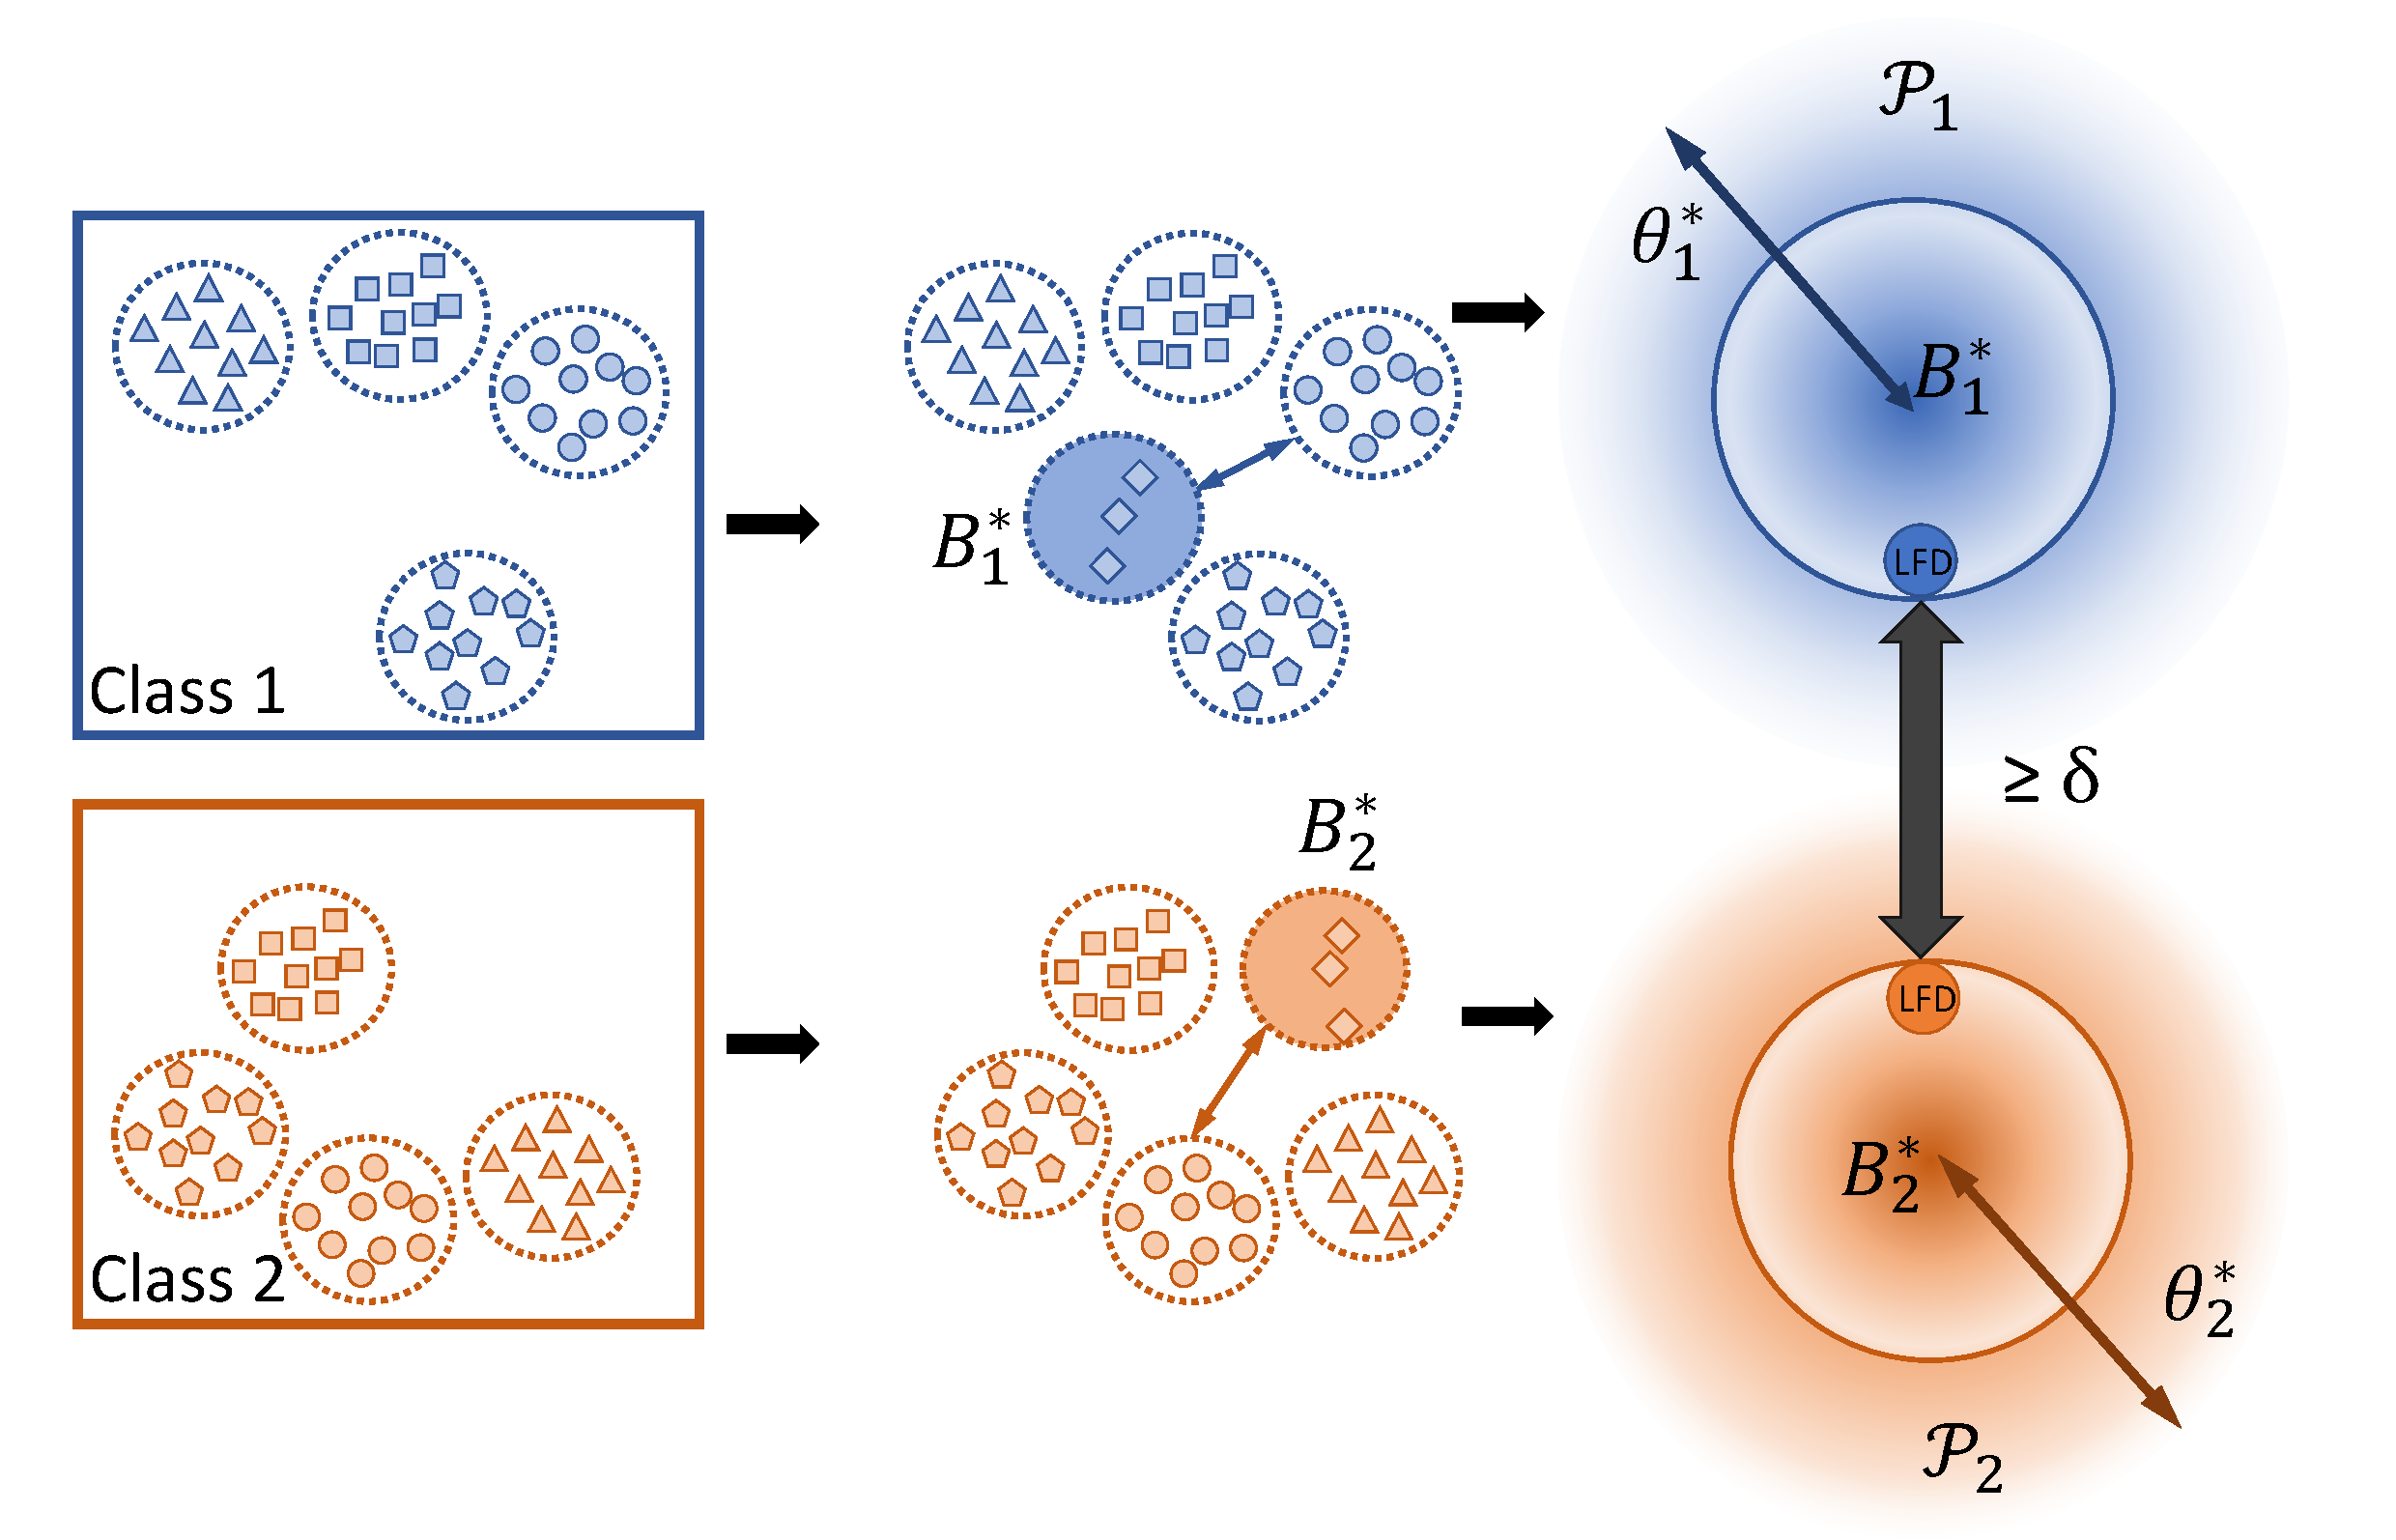
\includegraphics[width=0.45\linewidth]{figures/pipeline/allinone-v220107-a-v4.pdf}
\label{subfig:a}}
\hfil
\subfloat[Distributionally robust optimization.]{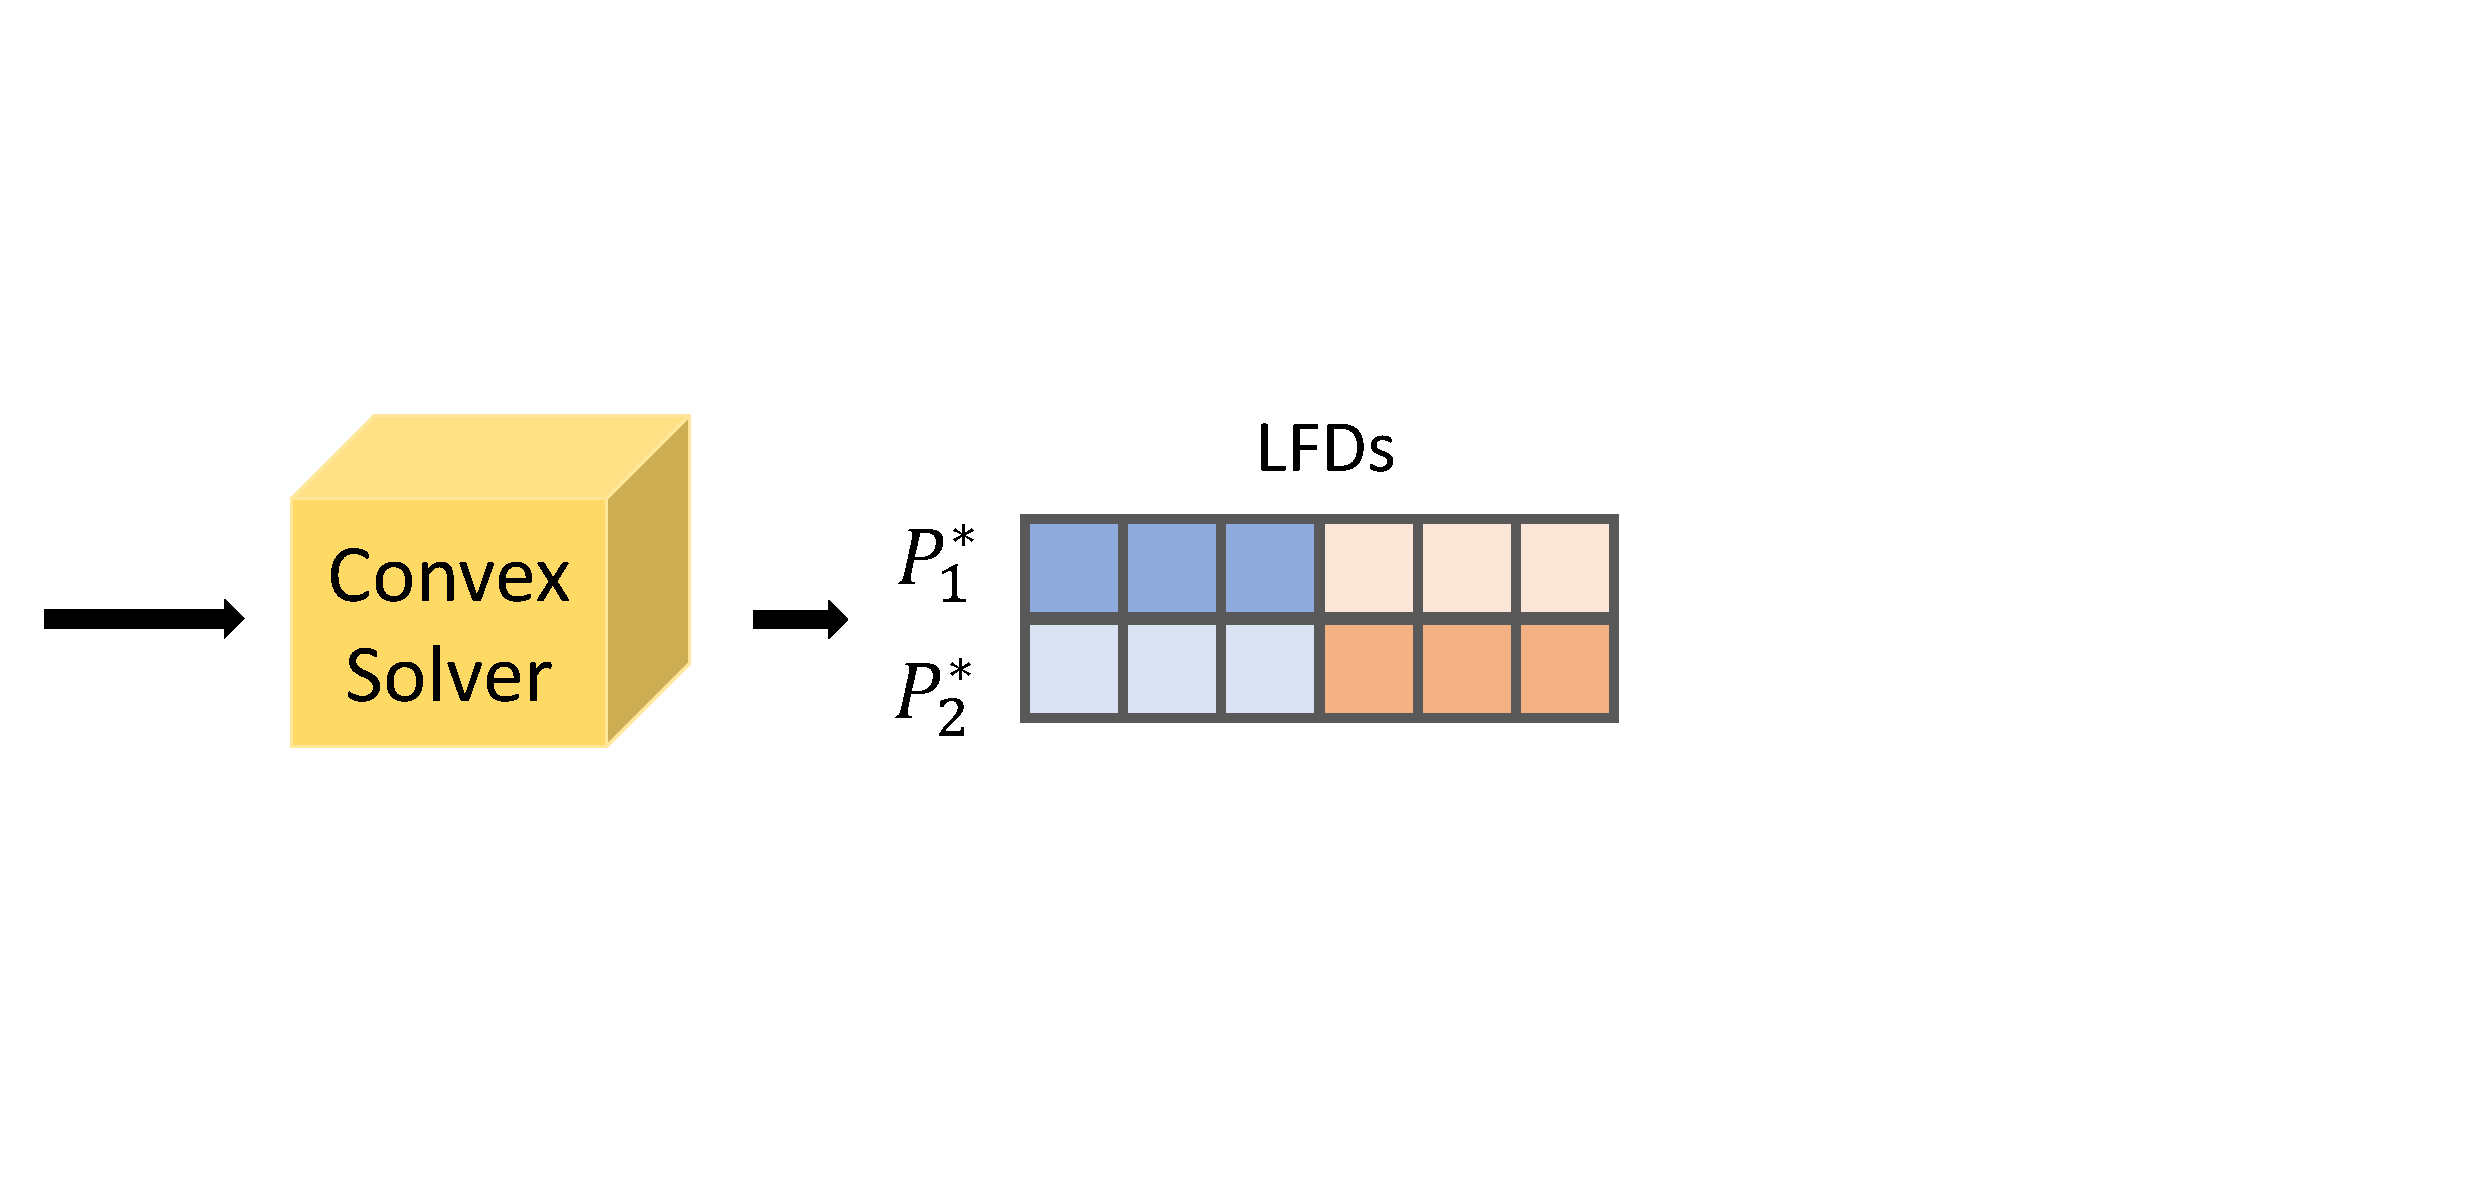
\includegraphics[width=0.45\linewidth]{figures/pipeline/allinone-v220107-b.pdf}
\label{subfig:b}}
\quad 
\subfloat[Adaptive inference using optimal transport.]{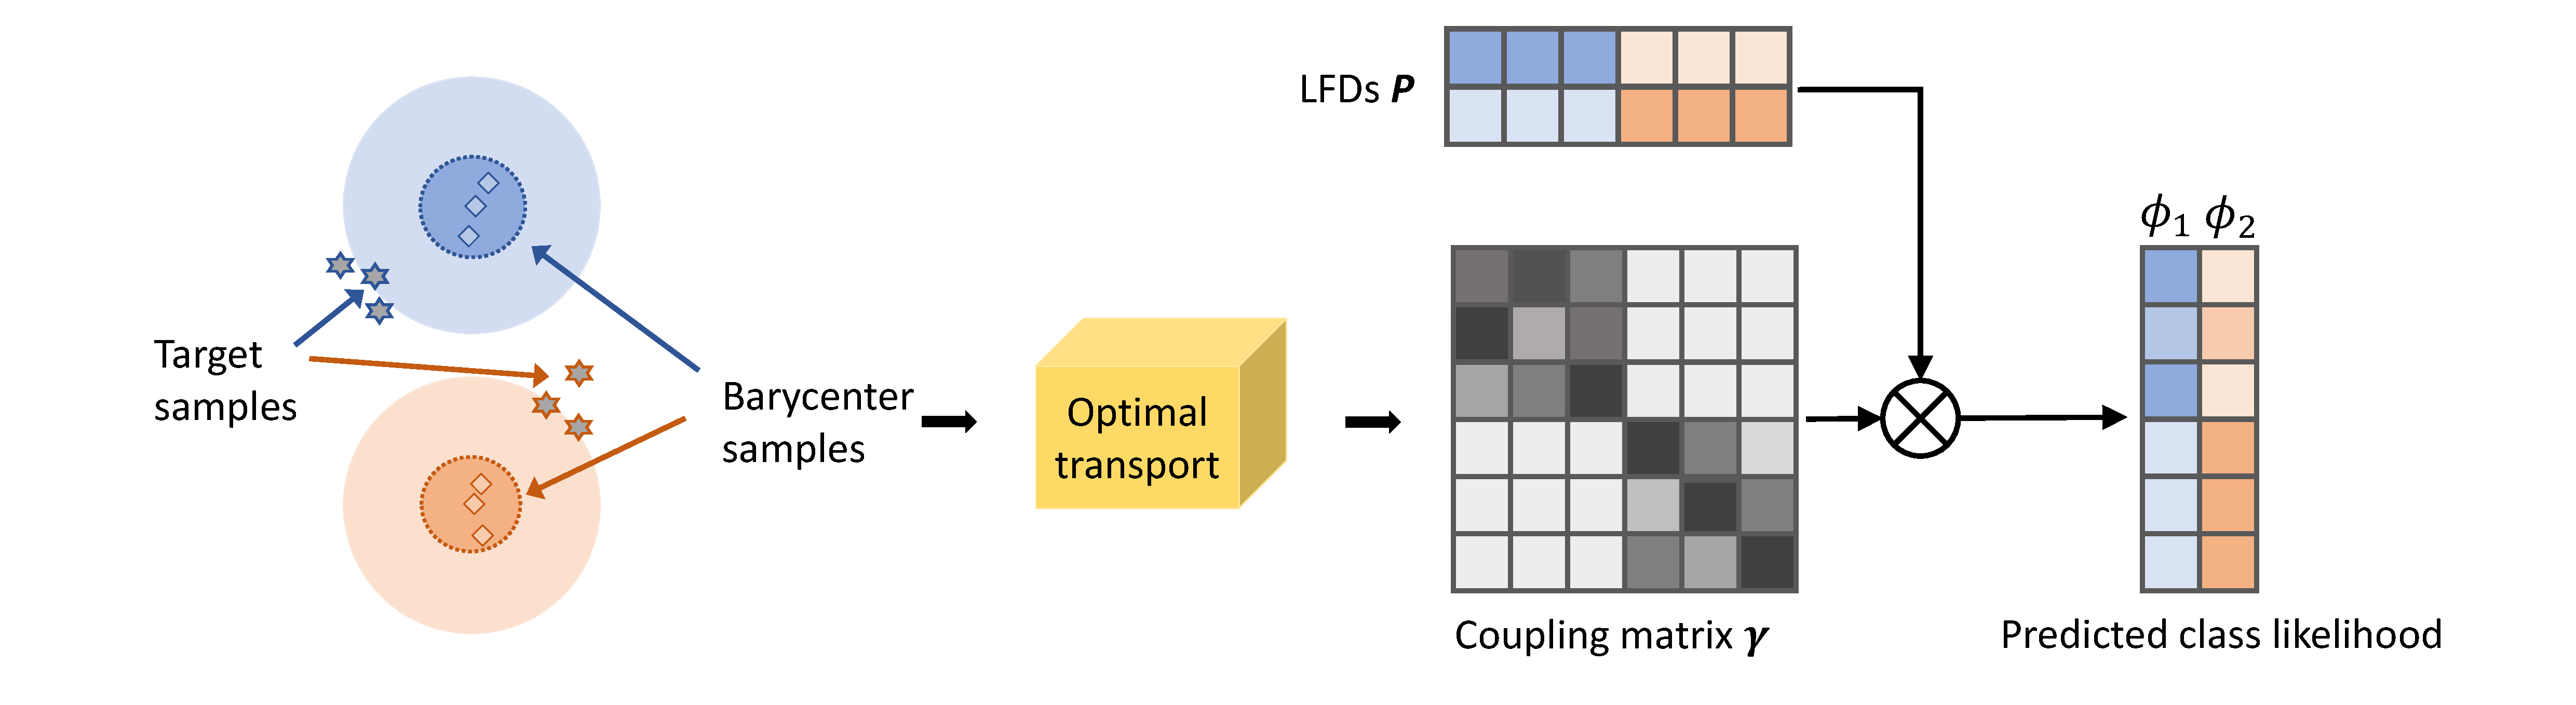
\includegraphics[width=0.85\linewidth]{figures/pipeline/allinone-v220107-c.pdf}
\label{subfig:c}}
\caption{An overview of our WDRDG framework, consisting of three components: (a) Wasserstein uncertainty set construction for each class based on the empirical Wasserstein barycenters and radius obtained from given source domains. One constraint is added to control the discriminability of LFDs; (b) distributionally robust optimization to solve for the least favorable distributions; 
% (c) optimal transportation between barycenter samples and target samples to learn 
% the optimal coupling matrix; 
(c) adaptive inference for target testing samples based on probability mass on LFDs and coupling matrix from  optimal transportation between barycenter samples and target samples.
% as in equation (\ref{eq:classifier})
}
\label{fig_sim}
\end{figure*}

\section{Wasserstein Distributionally Robust Domain Generalization}
In this section, we present our proposed framework for domain generalization that leverages the empirical distributions from multiple source domains as shown in Figure \ref{subfig:a}, and the process of distributionally robust optimization is shown in Figure \ref{subfig:b}.
The adaptive inference for the target domain is shown in Figure \ref{subfig:c}. 
Here we show binary classification for simplicity.

More specifically, we first extrapolate the class-conditional source distributions to a Wasserstein uncertainty set for each class. Figure \ref{subfig:a} illustrates the construction of uncertainty sets of two classes. Their closeness is further controlled by the parameter $\delta$ to ensure discriminability. A convex solver then solves the distributionally robust optimization over these uncertainty sets, obtaining
the least favorable distributions (LFDs), which are represented as probability mass vectors depicted in Figure \ref{subfig:b}. Figure 
\ref{subfig:c} shows the inference process for target samples, where optimal transport \cite{courty2016optimal} is used to re-weight LFDs adaptively. 

Details of the construction of uncertainty sets and the additional Wasserstein constraints could be found in Sections \ref{method:1} and \ref{method:2}. Section \ref{method:3} discusses the re-formulation of the Wasserstein robust optimization. Adaptive inference for samples in the target domain is presented in section \ref{methodSection:adaptive}. In \ref{sec:bound}, we further analyze the generalization bound of the proposed framework.



\subsection{Construction of Uncertainty Sets}\label{method:1}
We construct the uncertainty sets controlled 
% An uncertainty set is determined 
mainly by two terms: the reference distribution that represents the center of the uncertainty set,
and the radius parameter that controls the size of the set, i.e., an upper bound of the divergence between the reference distribution and other distributions in the set. 
We use {\it Wasserstein barycenter} \cite{rabin2011wasserstein}  as the reference distribution, which is the average of multiple given distributions and is capable of leveraging the inherent geometric relations among them \cite{zhou2020domain}. Given empirical class-conditional distributions $\widehat{Q}^{s_1}_k,$ $\ldots,$ $\widehat{Q}^{s_R}_k$ for each class $k$ from $R$ different source domains, the Wasserstein barycenter for class $k$ is defined as
\begin{equation} 
B^{*}_k= \underset{B_k}{\arg \min }\sum_{r=1}^{R} \frac{1}{R} \mathcal{W}_2( B_k,\widehat{Q}^{s_r}_k), k = 1,\ldots, K,
\label{eq:barycenter}
\end{equation}
which could be a proxy of the reference distribution for each uncertainty set. 
% Note that the support for each empirical barycenter could be decided according to actual demand.
Suppose each barycenter supports on $b$ samples uniformly, i.e., $B_k= \sum_{i=1}^{b}\frac{1}{b} \delta_{\boldsymbol{x}_i^{(k)}}$, where $\{\boldsymbol{x}_i^{(k)}\}_{i=1}^{b}$ are the barycenter samples for class $k$,
then (\ref{eq:barycenter}) only optimizes over the locations $\boldsymbol{x}_i^{(k)}$.

To ensure that the uncertainty sets are large enough 
% that allow for the most possible robustness from limited source knowledge
to avoid misclassification for unseen target samples, the maximum of all $R$ Wasserstein distances between class-conditional distributions of each source domain $\widehat{Q}^{s_r}_k$ and the  barycenter $B_k^*$,
is used as the radius for each class $k$:
\begin{equation}
\begin{aligned}
    \theta_k^*=\max\limits_{r=1,\ldots,R}\mathcal{W}_2\left(B^*_k, \widehat{Q}^{s_r}_k\right).
    \label{eq:radius}
\end{aligned}
\end{equation}
% \begin{equation}
%     \theta_k=\max\limits_{r=1,\cdots,R}\mathcal{W}_{2}\left(B^*(X|k), Q^{s_r}(X|k)\right), k=1,\cdots,K.\label{eq:radius}
% \end{equation}
In this way, we can construct the Wasserstein uncertainty set $\mathcal{P}_{k}$ of radius $\theta_k^*$ centered around $B^{*}_k$ for each class $k$ following \eqref{eq:uncertainty_set}:
\begin{equation}
  \mathcal{P}_k=\left\{P_k\in \mathscr{P}(\widehat{\mathcal{X}}): \mathcal{W}_2\left(P_k, {B}_k^*\right) \leq \theta_k^*\right\}.  
\end{equation}
Figure \ref{subfig:a} shows the construction process of the uncertainty sets for two classes. 


\subsection{Balance Robustness and Discriminability}\label{method:2}
When the source training samples are limited, 
the class-conditional distributions may
% When the randomly sampled source domain class-conditional distributions 
vary widely in practice. 
In this situation, the radius computed from (\ref{eq:radius}) tends to be overly large,
and the uncertainty sets of different classes may overlap with each other, leading to indistinguishable LFDs for optimization problem \eqref{eq:robustHT}.
As shown in Figure \ref{fig:radius_compare}, overlap between each pair of class-specific uncertainty sets exist as the sum of their radius is larger than the Wasserstein distance between the corresponding barycenters.



\begin{figure}[!t]
\centering
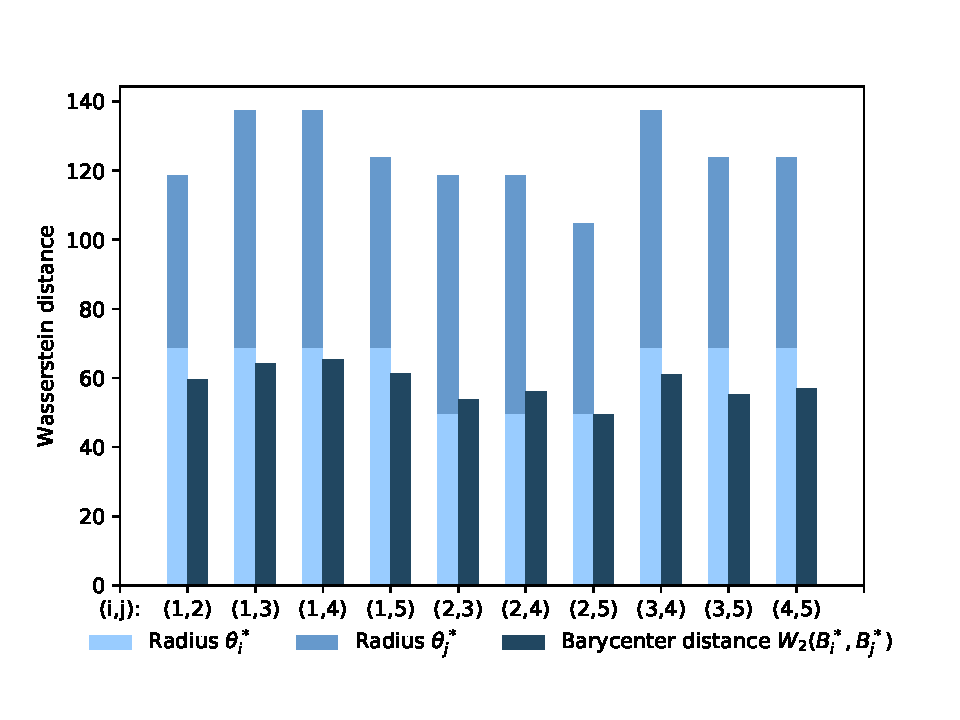
\includegraphics[width = 3.5in]{figures/radius/plot_radius.pdf}
\caption{Comparison between $\theta_i^*+\theta_j^*$ and the Wasserstein distance $W_2(B_i^*, B_j^*)$ for all $10$ unique pairs $(i,j)$ among all $5$ classes of the VLCS dataset.
The sum of uncertainty radius of any two classes is larger than the Wasserstein distance between the corresponding barycenters. The oversized radius will lead to overlapping class-specific uncertainty sets, and the distributions within them will be indistinguishable.
% Comparison between sum of uncertainty radius and the Wasserstein distance between each pair of barycenters.
% All $10$ unique pairs among $5$ classes in the VLCS dataset are shown.
}
\label{fig:radius_compare}
\end{figure}


% \begin{figure}[!t]
% \centering
% \includegraphics[width=2.5in]{myfigure}
% \caption{Simulation results for the network.}
% \label{fig_sim}
% \end{figure}

Discriminability of LFDs is necessary since this leads to a well-defined problem of \eqref{eq:robustHT}, which indirectly controls the discriminability of data from different classes.
% how to add wass constraint
We add one more constraint to obtain significantly different LFDs that are discriminable, characterized by the Wasserstein distance between each pair of LFDs $(P_u^*, P_v^*)$ within $K$ classes:
\begin{equation}
\label{eq:wass_constraint}
\mathcal{W}_2\left(P_u^*, P_v^*\right) \ge \delta, \  1\leq u < v \leq K,
\end{equation}
where $\delta>0$ is the threshold that indicates the discriminability, which could be tuned on a validation domain. 
In this way,  robustness is ensured by large enough Wasserstein uncertainty sets, and the threshold $\delta$ guarantees discriminability among the uncertainty sets. 


\subsection{Distributionally Robust Optimization}\label{method:3}
Incorporating the constraints (\ref{eq:wass_constraint}) into (\ref{eq:robustHT}), we aim to solve the following minimax problem
\begin{equation}
\label{eq:our_minimax}
\begin{aligned}
    & \min_{\phi:\mathcal{X}\rightarrow \Delta_K}  \max_{\substack{P_{k} \in \mathcal{P}_{k}, \ 1\leq k \leq K \\ 
    \mathcal{W}\left(P_u, P_v\right) \geq \delta, \ 1\leq u < v\leq K}}  \Psi\left(\phi; P_{1},\ldots, P_{K}\right).
\end{aligned}
\end{equation}
% where $\mathcal{P}_k=\left\{P_k\in \mathscr{P}(\widehat{\mathcal{X}}): \mathcal{W}_2\left(P_k, {B}_k^*\right) \leq \theta_k^*\right\}$.
We establish the following theorem, stating a convex approximation of problem \eqref{eq:our_minimax}.







\renewcommand{\algorithmicrequire}{ \textbf{Input:}}  
\renewcommand{\algorithmicensure}{ \textbf{Output:}}    %wjg 0903 UseOutput in the format of Algorithm
\begin{algorithm}[t]
  \caption{Wasserstein distributionally robust domain generalization.}
  \label{algorithm}
  \begin{algorithmic}[1]
  \REQUIRE  
  $\{\widehat{Q}^{s_r}_k\}_{r=1}^R$ - empirical class-conditional distributions for each class $k$ in all $K$ classes from source domains $\{\mathcal{D}^{s_r}\}_{r=1}^R$;\\
  $b$ - number of barycenter samples for each class;\\
  $\delta$ - discriminability threshold parameter.
  \ENSURE $\phi(\boldsymbol{x}^t_j)$ - predictions for each of the unseen target samples $\{\boldsymbol{x}_j^t\}_{j=1}^{n_t}$.
  %,\cdots,\boldsymbol{x}^t_{n_t}\}$.
  \FOR{each class $k$}
    \STATE Obtain barycenter $B^*_k$ by (\ref{eq:barycenter});\\
    \STATE Obtain radius $\theta_k^*$ using (\ref{eq:radius}).\\
    \STATE Construct uncertainty sets $\mathcal{P}_k$ centered around $B^*_k$ with radius $\theta_k^*$ as formed in (\ref{eq:uncertainty_set}).\\
  \ENDFOR
  \STATE Solve the optimization (\ref{eq:add_wass_all}) for the optimal LFDs ${P}^*_k$.\\
%   \STATE Transport target samples to barycenter samples using optimal transport with coupling matrix $\boldsymbol{\gamma}$.
%   \STATE Normalize the transport matrix.
  \STATE 
%   Re-weight the LFDs on barycenter samples by the coupling matrix, and get 
  The inference for each target sample is given by (\ref{eq:classifier}).
  \end{algorithmic}
\end{algorithm}


\begin{theorem}%[]
\label{theorem:add_wass_all}
Suppose the Wasserstein barycenter $B_k^\ast$ for each class as defined in (\ref{eq:barycenter}) is supported on $b$ samples. 
Let $S_b$ be the union of the support of $\{B_1^\ast,\ldots,B_K^\ast\}$ which contains ${n_b}=Kb$ samples $\{\boldsymbol{x}_i^b, i=1,\ldots,n_b\}$ in total. 
The class prior distributions of each class is denoted as $\mathbb{P}(y=k)$.
Denote each distribution within the uncertainty set $\mathcal{P}_k$ as $P_k\in\mathbb{R}_+^{n_b}$.
Let $\boldsymbol{C}\in \mathbb{R}_+^{{n_b}\times {n_b}}$ be the pairwise distance matrix of $n_b$ samples, $\boldsymbol{C}_{i,j} = \Vert \boldsymbol{x}_i^b - \boldsymbol{x}_j^b\Vert^2$, $\gamma_k\in\mathbb{R}_+^{{n_b}\times {n_b}}$ be the coupling matrix between $B_k^*$ and $P_k$, 
and $\beta_{u,v}\in\mathbb{R}_+^{{n_b}\times {n_b}}$ be the coupling matrix between any two distributions $P_u, P_v$ in different classes.
When using the Wasserstein metric of order 2, the least favorable distributions $P^*_k$ of the problem (\ref{eq:our_minimax}) could be obtained by solving: 
\begin{equation}
\label{eq:add_wass_all}
\begin{aligned}
%   \max_{\substack{P_1,\ldots,P_{K}\in\mathbb{R}_+^{{n_b}}\\\gamma_1,\ldots,\gamma_{K}\in\mathbb{R}_+^{{n_b}\times {n_b}}\\ \beta_{u,v}\in\mathbb{R}_+^{{n_b}\times {n_b}}}}
%   & K-\sum_{i=1}^{{n_b}}\max_{1\leq k \leq K}P_k\left(\boldsymbol{x}^b_i\right)\\
\max_{\substack{P_1,\ldots,P_{K}\in\mathbb{R}_+^{{n_b}}\\\gamma_1,\ldots,\gamma_{K}\in\mathbb{R}_+^{{n_b}\times {n_b}}\\ \beta_{u,v}\in\mathbb{R}_+^{{n_b}\times {n_b}}}}
  & 1-\sum_{i=1}^{{n_b}}\max_{1\leq k \leq K}\mathbb{P}(y=k) P_k\left(\boldsymbol{x}^b_i\right)\\
  \text { s.t. } 
  & \left\langle{\gamma}_k,\boldsymbol{C}\right\rangle_F\leq (\theta_k^*)^2,\left\langle{\beta}_{u,v},\boldsymbol{C}\right\rangle_F\geq \delta^2,\\
  & {\gamma}_k \boldsymbol{1}_{{n_b}}=B_k^*,{\gamma}_k^T \boldsymbol{1}_{{n_b}}=P_k,\\
  & {\beta}_{u,v} \boldsymbol{1}_{{n_b}}=P_u,{\beta}_{u,v}^T \boldsymbol{1}_{{n_b}}=P_v,\\
%   & \!\sum_{l=1}^{n}\sum_{m=1}^{n} \gamma_{k, l, m} c(x_l,x_m)\leq \theta_k,\\
%   & \!\sum_{l=1}^{n}\sum_{m=1}^{n} \beta_{[u,v], l, m} c(x_l,x_m)\geq \delta,\\
%   & \!\sum_{m=1}^{n}\gamma_{k, l, m}= Q_{k}^l, \sum_{l=1}^{n}\gamma_{k, l, m}=p_k^m,\\
% %   & \!\sum_{l=1}^{n}\gamma_{k, l, m}=p_k^m,\\
%   & \!\sum_{m=1}^{n}\beta_{[u,v], l, m}=p_u^l, \sum_{l=1}^{n}\beta_{[u,v], l, m}=p_v^m,\\
%   & \!\sum_{l=1}^{n}\beta_{[u,v], l, m}=p_v^m,\\
  & \forall 1 \leq k \leq K, 1\leq u< v \leq K,
\end{aligned}
\end{equation}
and the optimal prediction function of (\ref{eq:our_minimax}) satisfies
$\phi^*_k(\boldsymbol{x}_i^b)={P_{k}^{*}\left(\boldsymbol{x}_i^b\right)}/{\sum_{k=1}^{K}P_{k}^{*}\left(\boldsymbol{x}_i^b\right)}$ for any $\boldsymbol{x}_i^b\in S_b$.
% $\phi^*_k$ assigns non-zero probability for any $\boldsymbol{x}_l$ in $S$ if $\phi^{*}_k(\boldsymbol{x}_l)>0$ for $k\subset \arg\max_{k}P_k(\boldsymbol{x}_l)$.
\end{theorem}
\noindent
The constraints on $\gamma_k$ restrict each target class-conditional distribution to its respective uncertainty set of radius $\theta_k^*$.
% The first line of the constraints controls the possible distributions within each uncertainty set of radius $\theta_k$ centered around $B_k$.
The constraints on $\beta_{u,v}$ restrict the Wasserstein distance between each pair of class-conditional distributions in the target domain following \eqref{eq:wass_constraint}.
Based on the above theorem,
% Theorem \ref{theorem:add_wass_all}, 
the classification for any sample in the sample set $S_b$ is given by $\Phi(\boldsymbol{x}_i^b)=\arg\max_{1\leq k\leq K}P^*_k(\boldsymbol{x}_i^b)$.
{The proof can be found in 
% Section \ref{proof:add_wass_all} of 
the supplementary material.}



% \subsection{Adaptive Inference via Optimal Transport}
\subsection{Adaptive Inference by Test-time  Adaptation}

\label{methodSection:adaptive}
% According to \cite{gao2018robust}, when setting the auxiliary function as $2\min{(p,1-p)}$ in binary robust hypothesis testing, the corresponding optimal detector is $\text{sgn}\left({p_1}-{p_2}\right)$.
Since the barycenters are the weighted average of distributions from multiple source domains, the barycenter samples in the support set $S_b$ could be viewed as samples from a {\it generalized source domain} denoted as $\mathcal{D}^{b}$. 
For any sample in $\mathcal{D}^{b}$, the likelihood that it is assigned to each class could be decided based on $\phi^*$ %trained on %$\mathcal{D}^{b}$ and 
%labeled samples in $S_b$ \cite{zhu2020distributionally}.  As $\phi^*$ is a non-parametric function of samples in $S_b$, 
by a non-parametric  inference method such as KNN \cite{zhu2020distributionally}. %While 
When making predictions for samples from an unseen target domain $D^t$, the domain shift between $\mathcal{D}^{b}$ and $D^t$ needs to be considered. We adopt optimal transport   to reduce the domain shift adaptively by the following test-time adaptation process.



Suppose $\widehat{\mu}_{b}=\sum_{i=1}^{n_{b}}\frac{1}{n_{b}} \delta_{\boldsymbol{x}_i^{b}}$ and $\widehat{\mu}_{t}=\sum_{j=1}^{n_t}\frac{1}{n_t} \delta_{\boldsymbol{x}_j^{t}}$ are the empirical marginal distributions of the feature vectors from the generalized source domain $\mathcal{D}^{b}$ and a target domain $\mathcal{D}^t$, respectively.
% which could be written as empirical distributions when discrete samples are accessible, i.e.,   
% $\mu_{s}=\sum_{i=1}^{n_s}\frac{1}{n_s} \delta_{\boldsymbol{x}_i^{s}}$,  $\mu_{t}=\sum_{j=1}^{n_t}\frac{1}{n_t} \delta_{\boldsymbol{x}_j^{t}}$,
Denote the coupling matrix of transporting from target to the generalized source distribution using optimal transport \cite{courty2016optimal}
as $\boldsymbol{\gamma}=[{\gamma}_1,\ldots,{\gamma}_{n_t}]^T\in\mathbb{R}^{n_t \times n_b}$, where each vector ${\gamma}_{j}\in\mathbb{R}^{n_b}$, $j=1,\ldots,n_t$, represents the transported mass from
the $j$-th target sample to each of the $n_b$ barycenter samples.
In most optimal transport-based domain adaptation methods, each target sample $\boldsymbol{x}_j^{t}$, $j=1,\ldots, n_t$, is first transported to $\widehat{\boldsymbol{x}}_j^{t}$ in the generalized source domain $\mathcal{D}^{b}$ by the barycentric mapping:
% \cite{courty2016optimal}: 
% $\widehat{\boldsymbol{x}}_j^{t}=\sum_{i=1}^{n_b}n_t {\boldsymbol{\gamma}}_{j,i}{\boldsymbol{x}_i^{b}}$.
\begin{equation}
    \widehat{\boldsymbol{x}}_j^{t}=\sum_{i=1}^{n_b}n_t {\boldsymbol{\gamma}}_{j,i}{\boldsymbol{x}_i^{b}}, \ j=1,\ldots, n_t,\label{barycentric_mapping}
\end{equation}
then having its label inferred based on the classifier learned on the labeled samples.
Instead of such a two-step process, we propose an equivalent single-step inference process. The following proposition states the equivalence,
% When using the weight  $w\left(\widehat{\boldsymbol{x}}_j^{t},\boldsymbol{x}_i^{b}\right)=n_t \boldsymbol{\gamma}_{j,i}$ that measures the importance of each barycenter sample to the target sample,
% the class likelihood can be obtained by re-weighting $\phi^*_k(\boldsymbol{x}_i^b)$ of all the labeled samples $\boldsymbol{x}_i^b$s in the generalized source domain.
% This is equivalent to re-weighting LFDs on the barycenter samples using the coupling matrix, without actually transporting the target samples to the generalized source domain.
and the proof can be found in the supplementary.
% appendix \ref{proof:equivalent}.

\begin{proposition}%[]
\label{proposition: equivalent}
Given the coupling matrix $\boldsymbol{\gamma}\in\mathbb{R}^{n_t \times n_b}$. Suppose we transport the target sample $\boldsymbol{x}_j^{t}$ from the empirical target distribution $\widehat{\mu}_{t}=\sum_{j=1}^{n_t}\frac{1}{n_t} \delta_{\boldsymbol{x}_j^{t}}$ to the generalized source domain empirical distribution $\widehat{\mu}_{b}=\sum_{i=1}^{n_{b}}\frac{1}{n_{b}} \delta_{\boldsymbol{x}_i^{b}}$ 
% $\widehat{\boldsymbol{x}}_j^{t}$ in
by the barycentric mapping as shown in (\ref{barycentric_mapping}), and obtain the class likelihood by re-weighting $\phi^*_k(\boldsymbol{x}_i^b)$ of all the samples $\boldsymbol{x}_i^b \in S_b$ using the weight function $w\left(\widehat{\boldsymbol{x}}_j^{t},\boldsymbol{x}_i^{b}\right)=n_t \boldsymbol{\gamma}_{j,i}$.
% classifying it by a weighted vote of LFDs on the samples from the generalized source domain using the weight function 
% $w\left(\widehat{\boldsymbol{x}}_j^{t},\boldsymbol{x}_i^{b}\right)=n_t \boldsymbol{\gamma}_{j,i}$,
Then the resulting classifier is equivalent to directly re-weighting LFDs on the barycenter samples using the coupling matrix. The equivalent classification result is:
\begin{equation}
    \Phi(\boldsymbol{x}^t_j)=\underset{1 \leq k \leq K}{\arg \max }\sum_{i=1}^{n_b}{\boldsymbol{\gamma}_{j,i}} P^*_k(\boldsymbol{x}^{b}_{i}).
\end{equation}
\end{proposition}
This proposition illustrates that domain difference between target domain and generalized source domain can be eliminated by adaptively  applying the coupling matrix in the inference stage, without actually transporting the target samples to the generalized source domain.
% In this way, the domain shift between the target domain and generalized source domain is eliminated adaptively by applying the coupling matrix in the inference stage.

% \noindent
% {The proof can be found in Section B of the supplementary material.}
% To make inference for target samples in our domain generalization setting, 
% we first obtain the optimal coupling matrix between the target distribution ${\mu}_t = \sum_{j=1}^{n_t}\frac{1}{n_t} \delta_{\boldsymbol{x}_j^t}$ and barycenter distribution ${\mu}_b = \sum_{i=1}^{n_b}
% \frac{1}{n_b}\delta_{\boldsymbol{x}_i^b}$ by optimal transport, denoted as 
% $\boldsymbol{\gamma}=[{\gamma}_1,\cdots,{\gamma}_{n_t}]^T\in\mathbb{R}^{n_t \times n_b}$, where each column vector ${\gamma}_{j}\in\mathbb{R}^{n_b}, j=1,\cdots,n_t$ represents the transported mass from the $j$-th
% target sample to each of the $n_b$ barycenter samples.

Denote the LFDs for all classes as $\boldsymbol{P}=\left[{P}_1^*,\ldots,{P}_K^*\right]^T\in\mathbb{R}^{K\times n_b}$.
% since the least favorable distributions are also supported on barycenters, each transport vector $\boldsymbol{w}_{i}, i = 1, \cdots, n_t$ is then normalized. 
Based on Proposition \ref{proposition: equivalent},
the predicted class likelihood of each target sample $\boldsymbol{x}^t_j$ can be written as
\begin{equation}
\label{eq:classifier}
\phi(\boldsymbol{x}^t_j)=\frac{ {{\boldsymbol{\gamma}_j}}^T \boldsymbol{P}^T}{ {{\boldsymbol{\gamma}_j}}^{T} \boldsymbol{P}^{T}\boldsymbol{1}_{K}}=\left[\phi_1(\boldsymbol{x}^t_j), \ldots, \phi_{K}\left(\boldsymbol{x}^t_j\right)\right],
% \phi(\boldsymbol{x}^t_j)= {\frac{\boldsymbol{w}_j}{\left| \boldsymbol{w}_j \right|}}^{\text{T}} \boldsymbol{P}^{\text{T}}=[\phi_1(\boldsymbol{x}^t_j), \cdots, \phi_K(\boldsymbol{x}^t_j)],
\end{equation}
% where the class likelihood $\phi$ gives the probability that the target sample $\boldsymbol{x}^t_i$ belongs to each of the $K$ categories,
where $0\leq \phi_k\left(\boldsymbol{x}^t_j\right)\leq 1, \sum_{k=1}^{K} \phi_k\left(\boldsymbol{x}^t_j\right) = 1$.
The algorithm is summarized in Algorithm \ref{algorithm}.
Further adding the optimal-transport based adaptive inference leads to our complete framework Wasserstein \textbf{D}istributionally \textbf{R}obust \textbf{D}omain \textbf{G}eneralization (\textbf{WDRDG}).
% that summarizes our overall framework.


\subsection{Generalization Analysis}\label{sec:bound}

We further analyze the generalization risk of our proposed method.
Our analysis
% extends the original result in \cite{zhu2020distributionally} and 
considers the domain shift between the target domain and the generalized source domain. 

Based on (\ref{eq:classifier}), the classification decision for the test sample $\widehat{\boldsymbol{x}}_j^{t}$ in the target domain is based on the weighted average
\begin{equation}
\label{eq:argmax_reweight}
% \phi_k(\boldsymbol{x}^t_j)=\frac{{\sum_{i=1}^{n_b} n_t{\boldsymbol{\gamma}_{j,i}} P^*_k(\boldsymbol{x}^{b}_{i})} }{\sum_{k=0}^{K-1}\sum_{i=1}^{n_b} n_t{\boldsymbol{\gamma}_{j,i}} P^*_k(\boldsymbol{x}^{b}_{i})},
     \underset{1 \leq k \leq K}{\arg \max }\sum_{i=1}^{n_b} w\left(\widehat{\boldsymbol{x}}_j^{t},\boldsymbol{x}_i^{b}\right) P^*_k(\boldsymbol{x}^{b}_{i}).
\end{equation}
% % If we use only one barycenter sample that best matches the target sample, the classification becomes
% % % the optimal transport finds the only mapping barycenter for each target sample.
% % % Here we consider the nearest source sample for simplicity.
% % % i.e., making classification decisions by
% % \begin{equation}
% % \begin{aligned}
% %     \underset{1 \leq k \leq K}{\arg \max } \ \thinspace{w\left(\widehat{\boldsymbol{x}}_j^{t},\boldsymbol{x}_{\tau_1(\widehat{\boldsymbol{x}}_j^{t})}^{b}\right)} P^*_k\left(\boldsymbol{x}_{\tau_1(\widehat{\boldsymbol{x}}_j^{t})}^{b}\right),
% % \end{aligned}
% % \end{equation}
% % where $\boldsymbol{x}_{\tau_1(\widehat{\boldsymbol{x}}_j^{t})}^{s}$ is the nearest neighbor of $\widehat{\boldsymbol{x}}_j^{t}$ 
% where $\tau_1(\widehat{\boldsymbol{x}}_j^{t})$ represents the index of the sample found in the generalized source domain that best matches the target sample using the aforementioned weight function (i.e., the one with the largest weight).
% % $w\left(\widehat{\boldsymbol{x}}_j^{t},\boldsymbol{x}_i^{b}\right)$.
% % =n_t \boldsymbol{\gamma}_{j,i}$.
% %

Consider a binary classification problem with label set $\{0,1\}$.
% In this case, while 
Let $\phi(\boldsymbol{x})=[\phi_0(\boldsymbol{x}),\phi_1(\boldsymbol{x})]$ represents the prediction vector of $\boldsymbol{x}$ belonging to either classes.
% that each sample belongs to each class, 
%and the corresponding hypothesis is $h:\mathcal{X}\rightarrow [1,2]$.
% actually gives the probability that $\boldsymbol{x}$ belongs to class 1, i.e., $h(\boldsymbol{x})=\phi_1(\boldsymbol{x})$.
The true labeling function is denoted as $f:\mathcal{X}\rightarrow\{0,1\}$.
Considering the simple case that all classes are balanced, 
the expected risk that the correct label is not accepted for samples in any distribution $\mu$ is denoted as $\epsilon_{\mu}\left(\phi\right)=\mathbb{E}_{\boldsymbol{x}\sim\mu}[1-\phi_{f(\boldsymbol{x})}(\boldsymbol{x})]$.
We now present the following theorem stating the generalization bound.

\begin{theorem}
\label{theorem:bound}
% Assume that the posterior probability function $\eta_{k}( \boldsymbol{x})=\mathbb{P}[y=k |\boldsymbol{x}]$ is $L$-Lipschitz for some constant $L\ge 0$, i.e., $\left|\eta_{k}(\boldsymbol{x})-\eta_{k}\left(\boldsymbol{x}^{\prime}\right)\right| \leq L\cdot c(\boldsymbol{x},\boldsymbol{x}')$,
% %L \left\Vert \boldsymbol{x}- \boldsymbol{x}'\right\Vert$.
% where $c$ denotes any metric function in the feature space.
% %that is inversely proportional to the weight function defined in Section \ref{methodSection:adaptive}.
% %The hypothesis $h$ is $M$-Lipschitz continuous for some $M$.
Suppose the distributionally robust prediction function $\phi^{S_b}$ learned from the sample set $S_b$ is $M$-Lipschitz continuous for some $M\geq0$.
Let $\mu_b$ and $\mu_t$ be the probability distributions for the generalized source and target domain, respectively.
% Let $\phi^{Bayes}$ be the prediction function for the Bayes optimal classifier, which assigns the class that has the largest posterior probability with probability 1. 
% Using the prediction function $\phi^{S_b}$ learned from the sample set $S_b$, 
Then the risk on the target distribution $\mu_t$ follows
\begin{equation}\label{eq:generalization}
\begin{aligned}
% \epsilon_{\mu_{t}}(\phi^{S_b}) 
% &\leq 2 \epsilon_{\mu_{b}}\left(\phi^{{Bayes}}\right) + L \cdot \underset{\boldsymbol{x}\sim \mu_{b}}{\mathbb{E}}\left[c\left(\boldsymbol{x}, \boldsymbol{x}_{\tau_{1}(\boldsymbol{x})}^{S_b}\right)\right] \\
% &+2M \cdot \mathcal{W}_{1}\left(\mu_{b}, \mu_{t}\right)+\lambda,
\epsilon_{\mu_{t}}(\phi^{S_b}) 
&\leq \epsilon_{\mu_{b}}(\phi^{S_b}) + 2M \cdot \mathcal{W}_{1}\left(\mu_{b}, \mu_{t}\right)+\lambda,
\end{aligned}
\end{equation}
where $\lambda=\underset{\phi:\mathcal{X}\rightarrow [0,1], \Vert\phi\Vert_{\textrm{Lip}}\leq M}{\min}\left(\epsilon_{\mu_t}(\phi) + \epsilon_{\mu_b}(\phi)\right)$.
% $\lambda$ is the combined error $\lambda=\underset{\phi}{\min}\left(\epsilon_{\mu_t}(\phi) + \epsilon_{\mu_b}(\phi)\right)$.
\end{theorem}
\noindent
% The first term on the right side of \eqref{eq:generalization} represents the optimal Bayes risk on the barycenter distribution, i.e., $\epsilon_{\mu_{b}}(\phi^{{Bayes}})=\mathbb{E}_{\boldsymbol{x} \sim \mu_b}\left[1-\max _{1 \leq k \leq K} \eta_{k}(\boldsymbol{x})\right]$.
% The second term illustrates the importance of the  set $S_b$ sampled from the distribution $\mu_b$ on the generalized source domain, 
% which gets smaller as the size of $S_b$ gets larger \cite{shalev-shwartz_ben-david_2014}.
% % since the representative sample $\boldsymbol{x}_{\tau_{1}(\boldsymbol{x})}^{S_b}$ found in the sample set $S_b$ for each sample in the generalized domain will be closer.
The first term is the risk on the barycenter distribution $\mu_b$.
The second term shows that the divergence between the barycenter distribution and target distribution, measured by the Wasserstein distance (of order $1$).
% influences the success of generalization to the target domain.
This theorem shows that the generalization risk on the target domain is affected by
the Wasserstein distance between the barycenter distribution and the target distribution, which represents the gap between the generalized source domain and the target domain.
% This theorem highlights the importance of reducing the Wasserstein distance between the barycenter distribution and the target distribution, which is realized by the optimal transport-based test-time adaptation in our framework. 
% This result is one of the motivation of introducing optimal transport in the inference stage,
% as described in Section \ref{methodSection:adaptive}. 

By applying the concentration property of the Wasserstein distance \cite{bolley2007quantitative}, we can measure the generalization risk based on empirical Wasserstein distances similar to Theorem 3 in \cite{shen2018wasserstein}. Under the assumption of Theorem \ref{theorem:bound}, if the two probability distributions $\mu_b$ and $\mu_t$ satisfy $T_1(\xi)$ inequality \cite{bolley2007quantitative}, 
then for any $d^\prime > d$ and $\xi^\prime < \xi$, there exists some constant $N_0$ depending on $d^\prime$ such that for any $\varepsilon>0 $ and $\min (n_b, n_t) \geq N_{0} \max \left(\varepsilon^{-\left(d^{\prime}+2\right)}, 1\right)$,
with probability at least $1-\varepsilon$ the following holds for the risk on the target domain
\[
\begin{aligned}
%   \epsilon_{\mu_t}(\phi^{S_b}) &\leq 2 \epsilon_{{\mu_b}}\left(\phi^{Bayes}\right)+ L \cdot \underset{\boldsymbol{x}\sim \mu_b}{\mathbb{E}}\left[c\left(\boldsymbol{x}, \boldsymbol{x}_{\tau_{1}(\boldsymbol{x})}^{S_b}\right)\right]
%   +2M \mathcal{W}_{1}\left(\widehat{\mu}_{b}, \widehat{\mu}_{t}\right)+\lambda
%   +2 M \sqrt{2 \log \left(\frac{1}{\varepsilon}\right) / \xi^{\prime}}\left(\sqrt{\frac{1}{n_{b}}}+\sqrt{\frac{1}{n_{t}}}\right).\notag
\epsilon_{\mu_t}(\phi^{S_b}) \leq &  \epsilon_{\mu_b}(\phi^{S_b})
  +2M \mathcal{W}_{1}\left(\widehat{\mu}_{b}, \widehat{\mu}_{t}\right)+\lambda\\
  &
  +2 M \sqrt{2 \log \left(\frac{1}{\varepsilon}\right) / \xi^{\prime}}\left(\sqrt{\frac{1}{n_{b}}}+\sqrt{\frac{1}{n_{t}}}\right).\notag
\end{aligned}
\]
% The second term above could be bounded based on \cite{shalev-shwartz_ben-david_2014}, which gets smaller as the size of the sample set $S_b$ gets bigger.
Here $d$ denotes the dimension of the feature space. The last term illustrates the importance of getting more labeled samples from the generalized source domain.
This result show that reducing the Wasserstein distance between the barycenters and target distributions will lead to tighter upper bound for the risk of the learned model on the target domain.
% , which is consistent with the goal of our test-time domain adaptation module.
Therefore, it provides a theoretical motivation to our design of the test-time adaptation, which reduces such domain gap by optimal transport.
% More details of the proof could be found in \ref{proof:bound} of the supplementary material.
Details of the proof could be found in the supplementary material.




% An example of a floating figure using the graphicx package.
% Note that \label must occur AFTER (or within) \caption.
% For figures, \caption should occur after the \includegraphics.
% Note that IEEEtran v1.7 and later has special internal code that
% is designed to preserve the operation of \label within \caption
% even when the captionsoff option is in effect. However, because
% of issues like this, it may be the safest practice to put all your
% \label just after \caption rather than within \caption{}.
%
% Reminder: the "draftcls" or "draftclsnofoot", not "draft", class
% option should be used if it is desired that the figures are to be
% displayed while in draft mode.
%
%\begin{figure}[!t]
%\centering
%\includegraphics[width=2.5in]{myfigure}
% where an .eps filename suffix will be assumed under latex, 
% and a .pdf suffix will be assumed for pdflatex; or what has been declared
% via \DeclareGraphicsExtensions.
%\caption{Simulation results for the network.}
%\label{fig_sim}
%\end{figure}

% Note that the IEEE typically puts floats only at the top, even when this
% results in a large percentage of a column being occupied by floats.
% However, the Computer Society has been known to put floats at the bottom.


% An example of a double column floating figure using two subfigures.
% (The subfig.sty package must be loaded for this to work.)
% The subfigure \label commands are set within each subfloat command,
% and the \label for the overall figure must come after \caption.
% \hfil is used as a separator to get equal spacing.
% Watch out that the combined width of all the subfigures on a 
% line do not exceed the text width or a line break will occur.
%
%\begin{figure*}[!t]
%\centering
%\subfloat[Case I]{\includegraphics[width=2.5in]{box}%
%\label{fig_first_case}}
%\hfil
%\subfloat[Case II]{\includegraphics[width=2.5in]{box}%
%\label{fig_second_case}}
%\caption{Simulation results for the network.}
%\label{fig_sim}
%\end{figure*}
%
% Note that often IEEE papers with subfigures do not employ subfigure
% captions (using the optional argument to \subfloat[]), but instead will
% reference/describe all of them (a), (b), etc., within the main caption.
% Be aware that for subfig.sty to generate the (a), (b), etc., subfigure
% labels, the optional argument to \subfloat must be present. If a
% subcaption is not desired, just leave its contents blank,
% e.g., \subfloat[].


% An example of a floating table. Note that, for IEEE style tables, the
% \caption command should come BEFORE the table and, given that table
% captions serve much like titles, are usually capitalized except for words
% such as a, an, and, as, at, but, by, for, in, nor, of, on, or, the, to
% and up, which are usually not capitalized unless they are the first or
% last word of the caption. Table text will default to \footnotesize as
% the IEEE normally uses this smaller font for tables.
% The \label must come after \caption as always.
%
%\begin{table}[!t]
%% increase table row spacing, adjust to taste
%\renewcommand{\arraystretch}{1.3}
% if using array.sty, it might be a good idea to tweak the value of
% \extrarowheight as needed to properly center the text within the cells
%\caption{An Example of a Table}
%\label{table_example}
%\centering
%% Some packages, such as MDW tools, offer better commands for making tables
%% than the plain LaTeX2e tabular which is used here.
%\begin{tabular}{|c||c|}
%\hline
%One & Two\\
%\hline
%Three & Four\\
%\hline
%\end{tabular}
%\end{table}


% Note that the IEEE does not put floats in the very first column
% - or typically anywhere on the first page for that matter. Also,
% in-text middle ("here") positioning is typically not used, but it
% is allowed and encouraged for Computer Society conferences (but
% not Computer Society journals). Most IEEE journals/conferences use
% top floats exclusively. 
% Note that, LaTeX2e, unlike IEEE journals/conferences, places
% footnotes above bottom floats. This can be corrected via the
% \fnbelowfloat command of the stfloats package.

\section{Experiments}

\subsection{Datasets}
To evaluate the effectiveness of our proposed domain generalization framework,
% the whole framework of applying DRO to domain generalization with the discriminability constraints and the optimal transport-based adaptive inference,
we conduct experiments on three datasets: 
the VLCS \cite{fang2013unbiased} dataset, the PACS \cite{li2017deeper} dataset, and the Rotated MNIST \cite{ghifary2015domain} dataset.
% As we assume limited labeled data from source domains, instances are sampled from each of the original datasets to model the small data scenarios.

\noindent
\textbf{VLCS dataset}
This domain generalization benchmark contains images from four image classification datasets: PASCAL VOC2007 (V), LabelMe (L), Caltech-101 (C), and SUN09 (S),
% PASCAL VOC2007 \cite{everingham2010pascal}, LabelMe \cite{russell2008labelme}, Caltech \cite{fei2004learning}, and SUN09 \cite{choi2010exploiting}, 
denoted as domains $D_V$, $D_L$, $D_C$, and $D_S$, respectively \cite{torralba2011unbiased}. 
There are five common categories: bird, car, chair, dog and person.
% Some example images of the VLCS dataset could be found in Figure \ref{fig:VLCS_dataset}.
% In each of the $5$ trials, we randomly sample up to $25$ training samples, $10$ validation samples, and $20$ testing samples for each of the 5 shared classes in every domain. 

\noindent
\textbf{PACS dataset}
The PACS dataset contains images of four domains: Photos (P), Art painting (A), Cartoon (C) and Sketch (S) \cite{li2017deeper}.
There are in total $7$ types of objects in this classification task, i.e., dog, elephant, giraffe, guitar, horse, house, and person. 
% Some example images could be found in Figure \ref{fig:intro_dg}.
% Similar as for the VLCS dataset, for the $7$ shared classes in each domain we randomly sample up to $25$ training samples, $10$ validation samples, and $20$ testing samples. This sampling process was also repeated $5$ times.


\noindent
\textbf{Rotated MNIST dataset}
We constructed the Rotated MNIST dataset with four domains, $r_0$, $r_{30}$, $r_{60}$ and $r_{90}$ following the common settings \cite{ghifary2015domain}.
% To be more specific, 
$r_0$ denotes the domain containing original images from the MNIST dataset, and
we rotated each image in the original MNIST dataset by $30$, $60$ and $90$ degrees clockwise, respectively to generate the dataset of $r_{30}$, $r_{60}$ and $r_{90}$.
Some example images are shown in Figure \ref{fig:rmnist_images}.
We randomly sampled 
% up to $25$ training images for each class as the training set, $10$ testing images per class as the validation set, and $20$ samples per class as the test set
among digits $[1, 2, 3]$.
% for each of the $5$ trials. 

\begin{figure}%[H]
  \centering
  \subfloat[$r_0$]
    {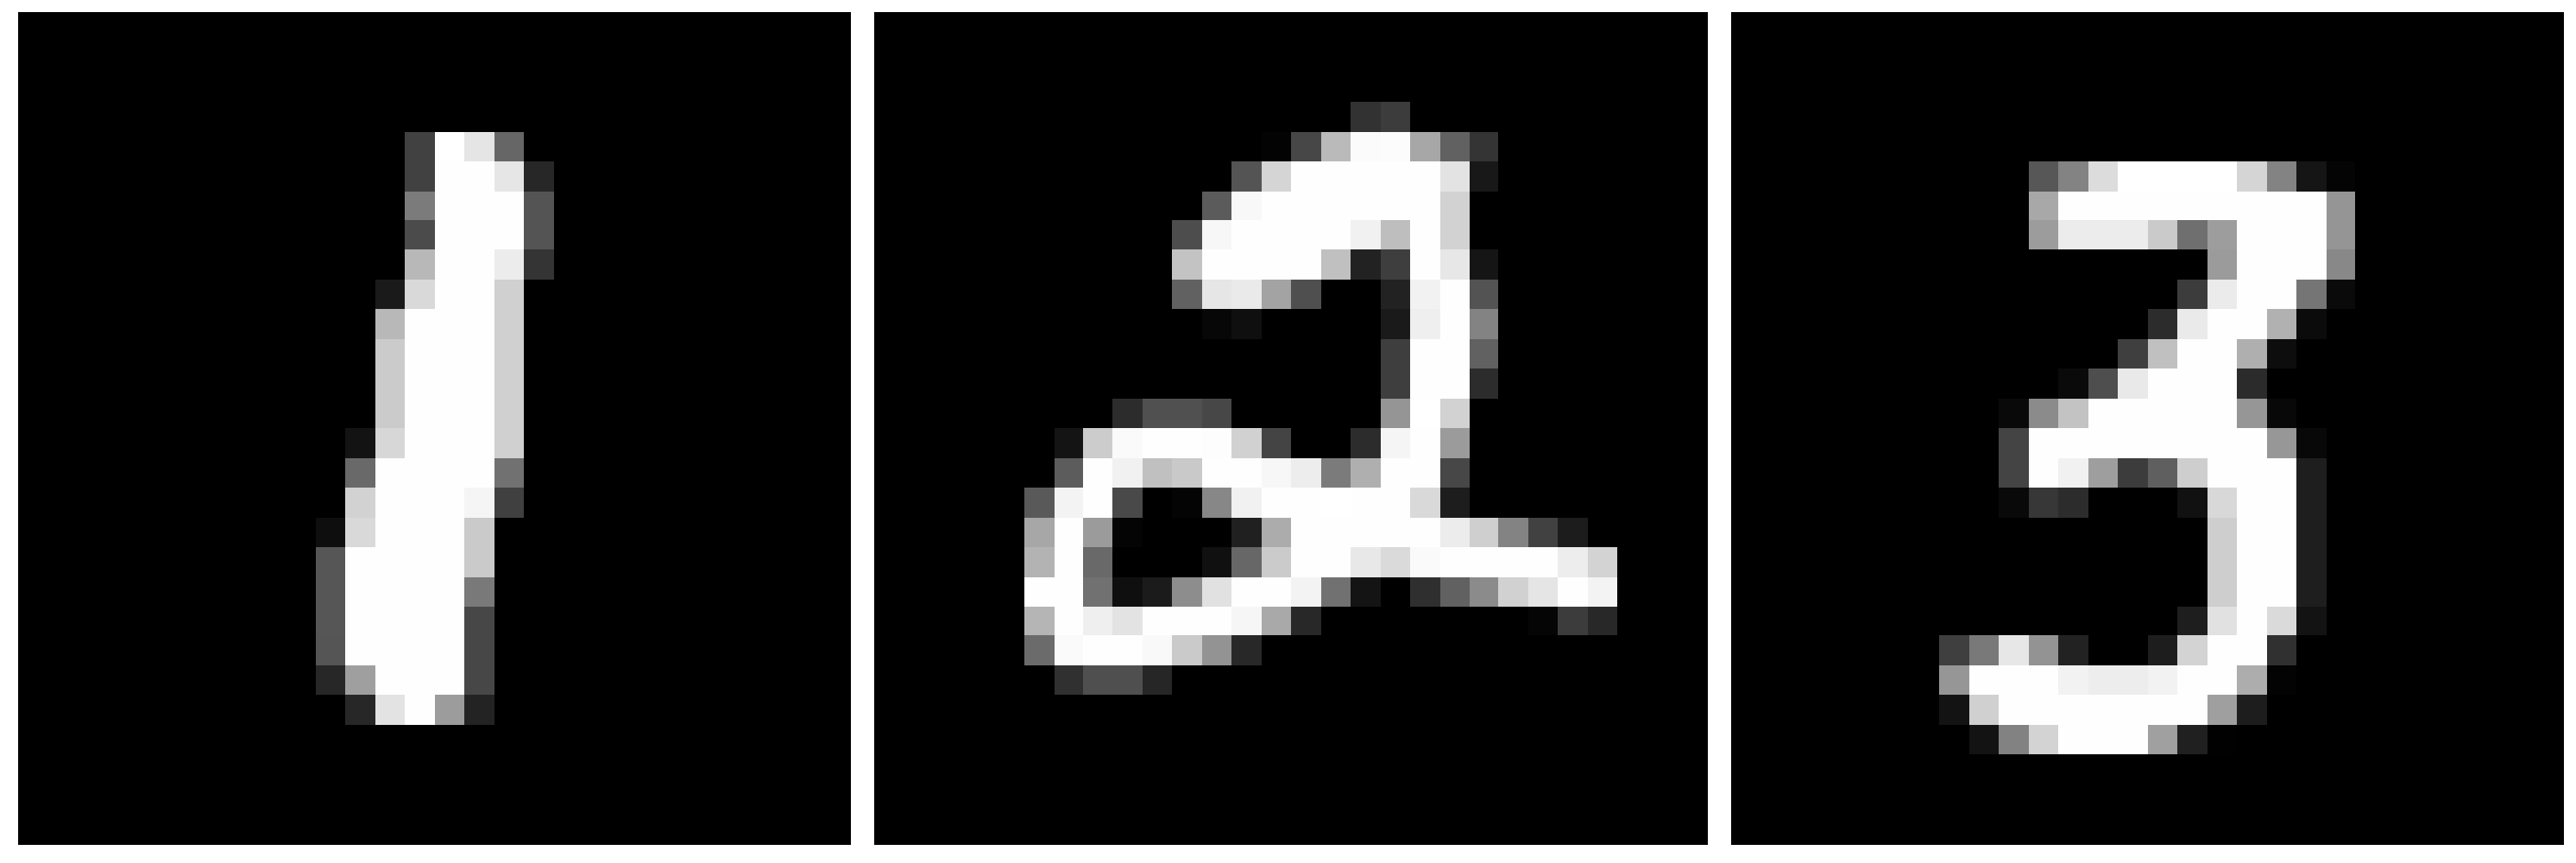
\includegraphics[width=0.3\linewidth]{figures/images/rmnist/rotation_0.pdf}\label{subfig:rmnist_images_0}}
  \subfloat[$r_{30}$]
    {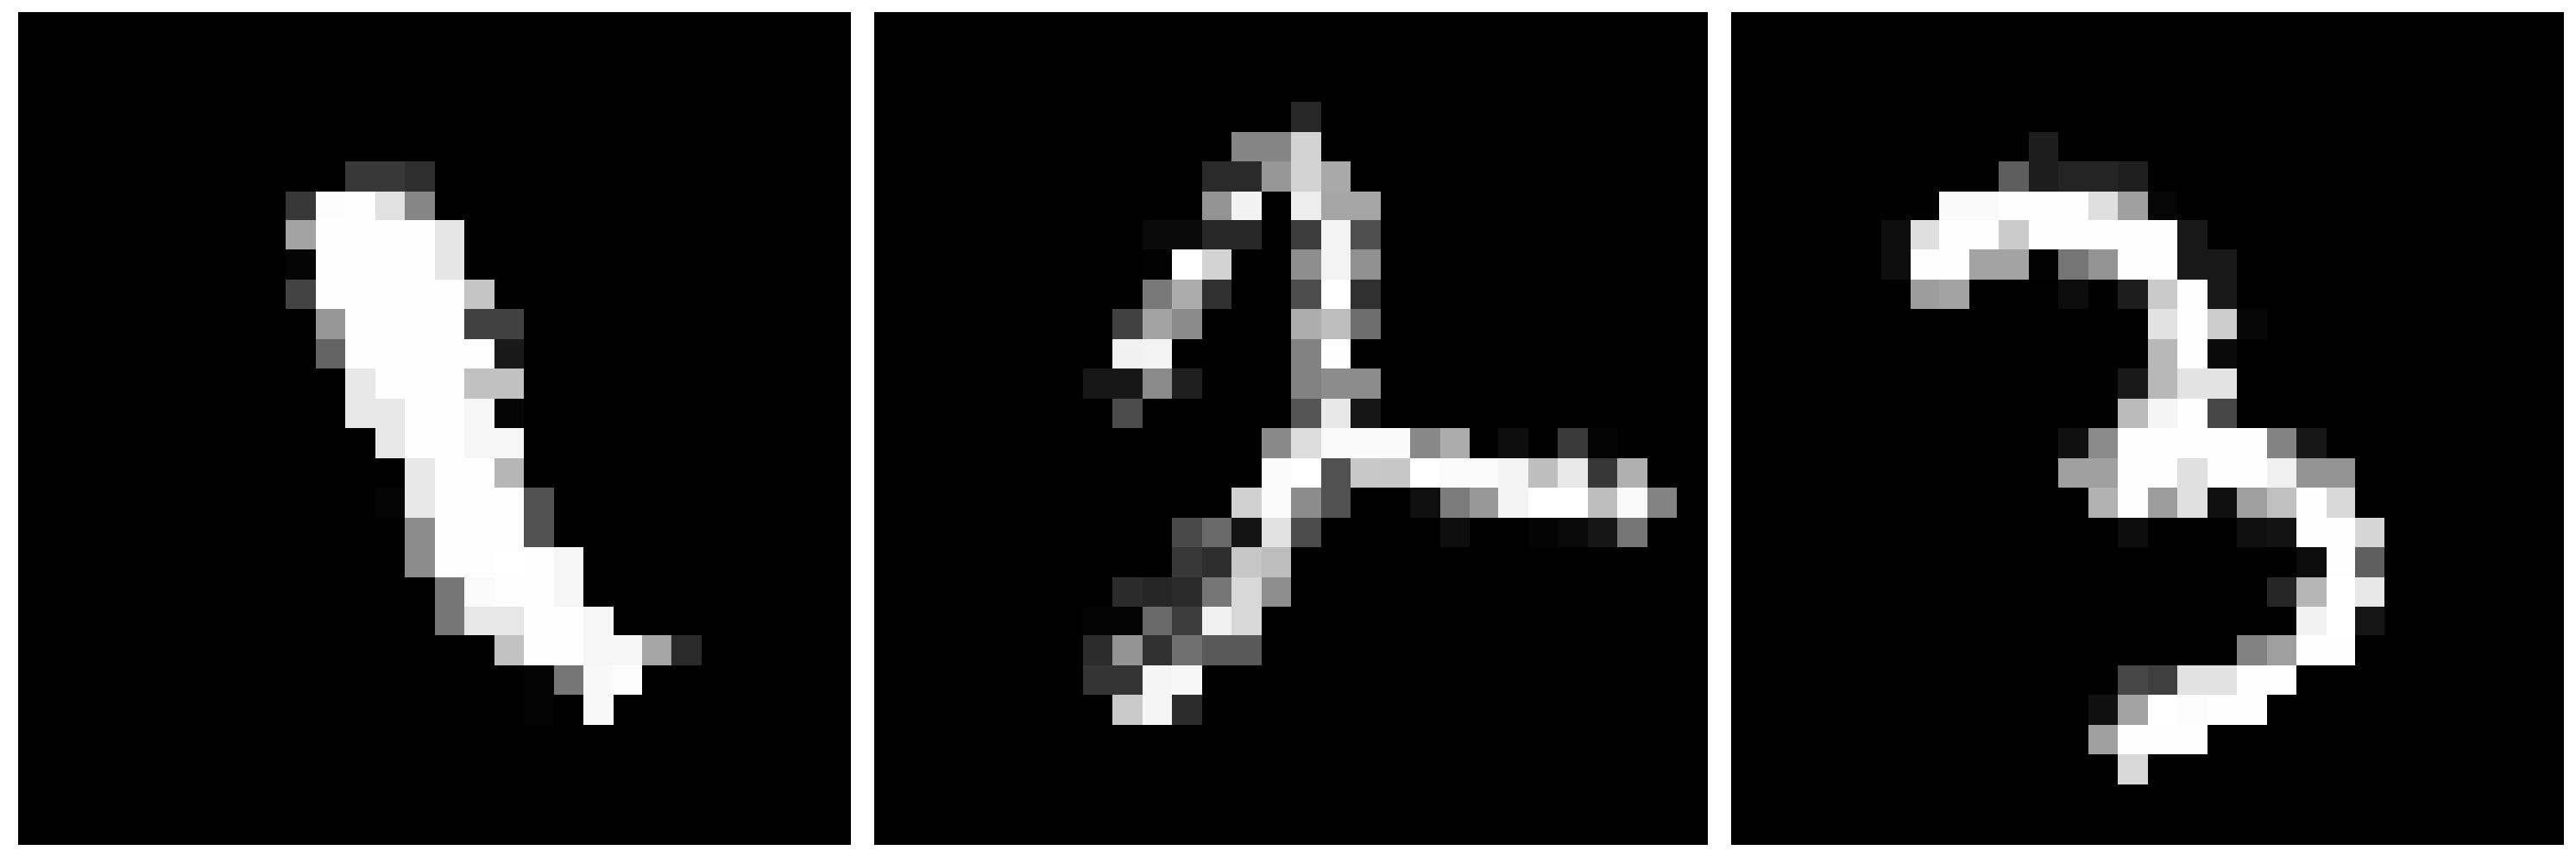
\includegraphics[width=0.3\linewidth]{figures/images/rmnist/rotation_30.pdf} \label{subfig:rmnist_images_30}}
  \quad 
  \subfloat[$r_{60}$]
    {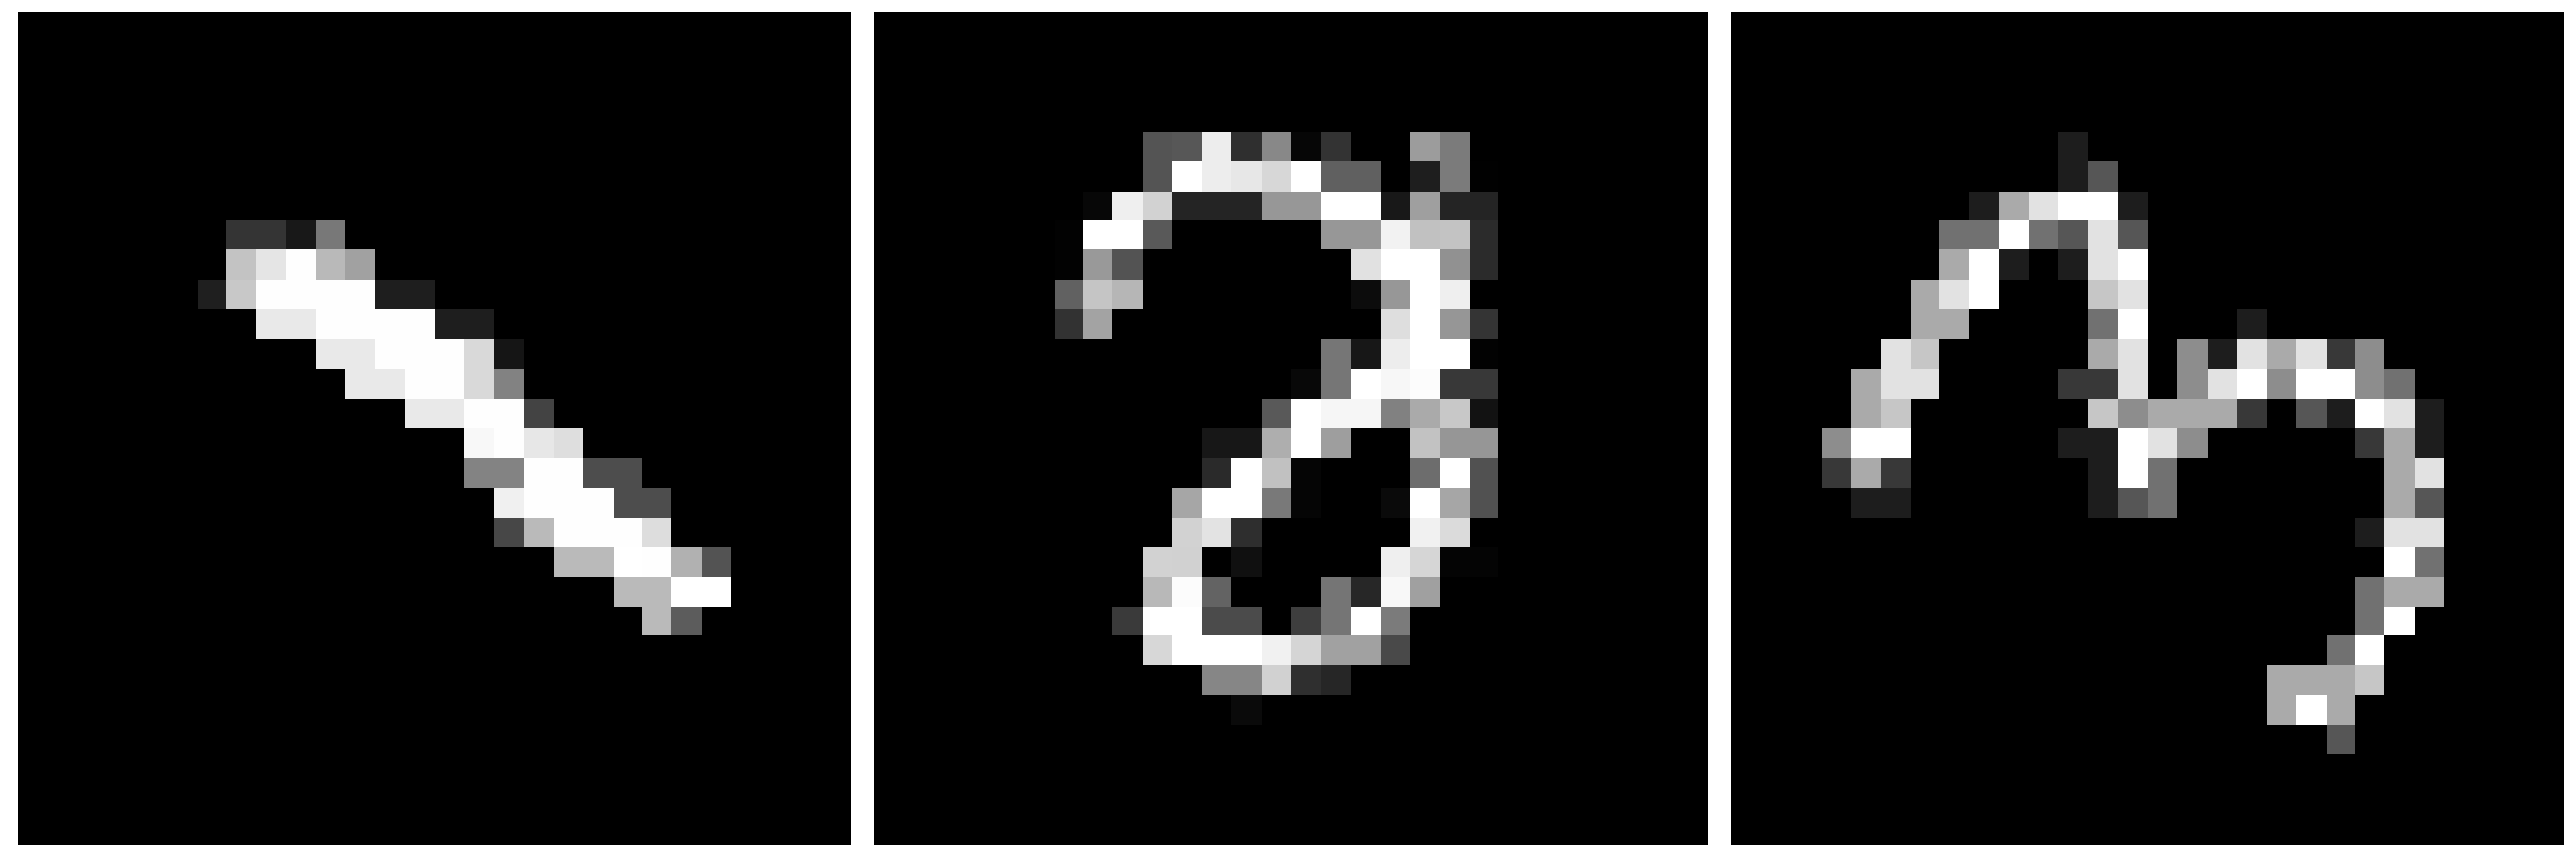
\includegraphics[width=0.3\linewidth]{figures/images/rmnist/rotation_60.pdf} \label{subfig:rmnist_images_60}}
  \subfloat[$r_{90}$]
    {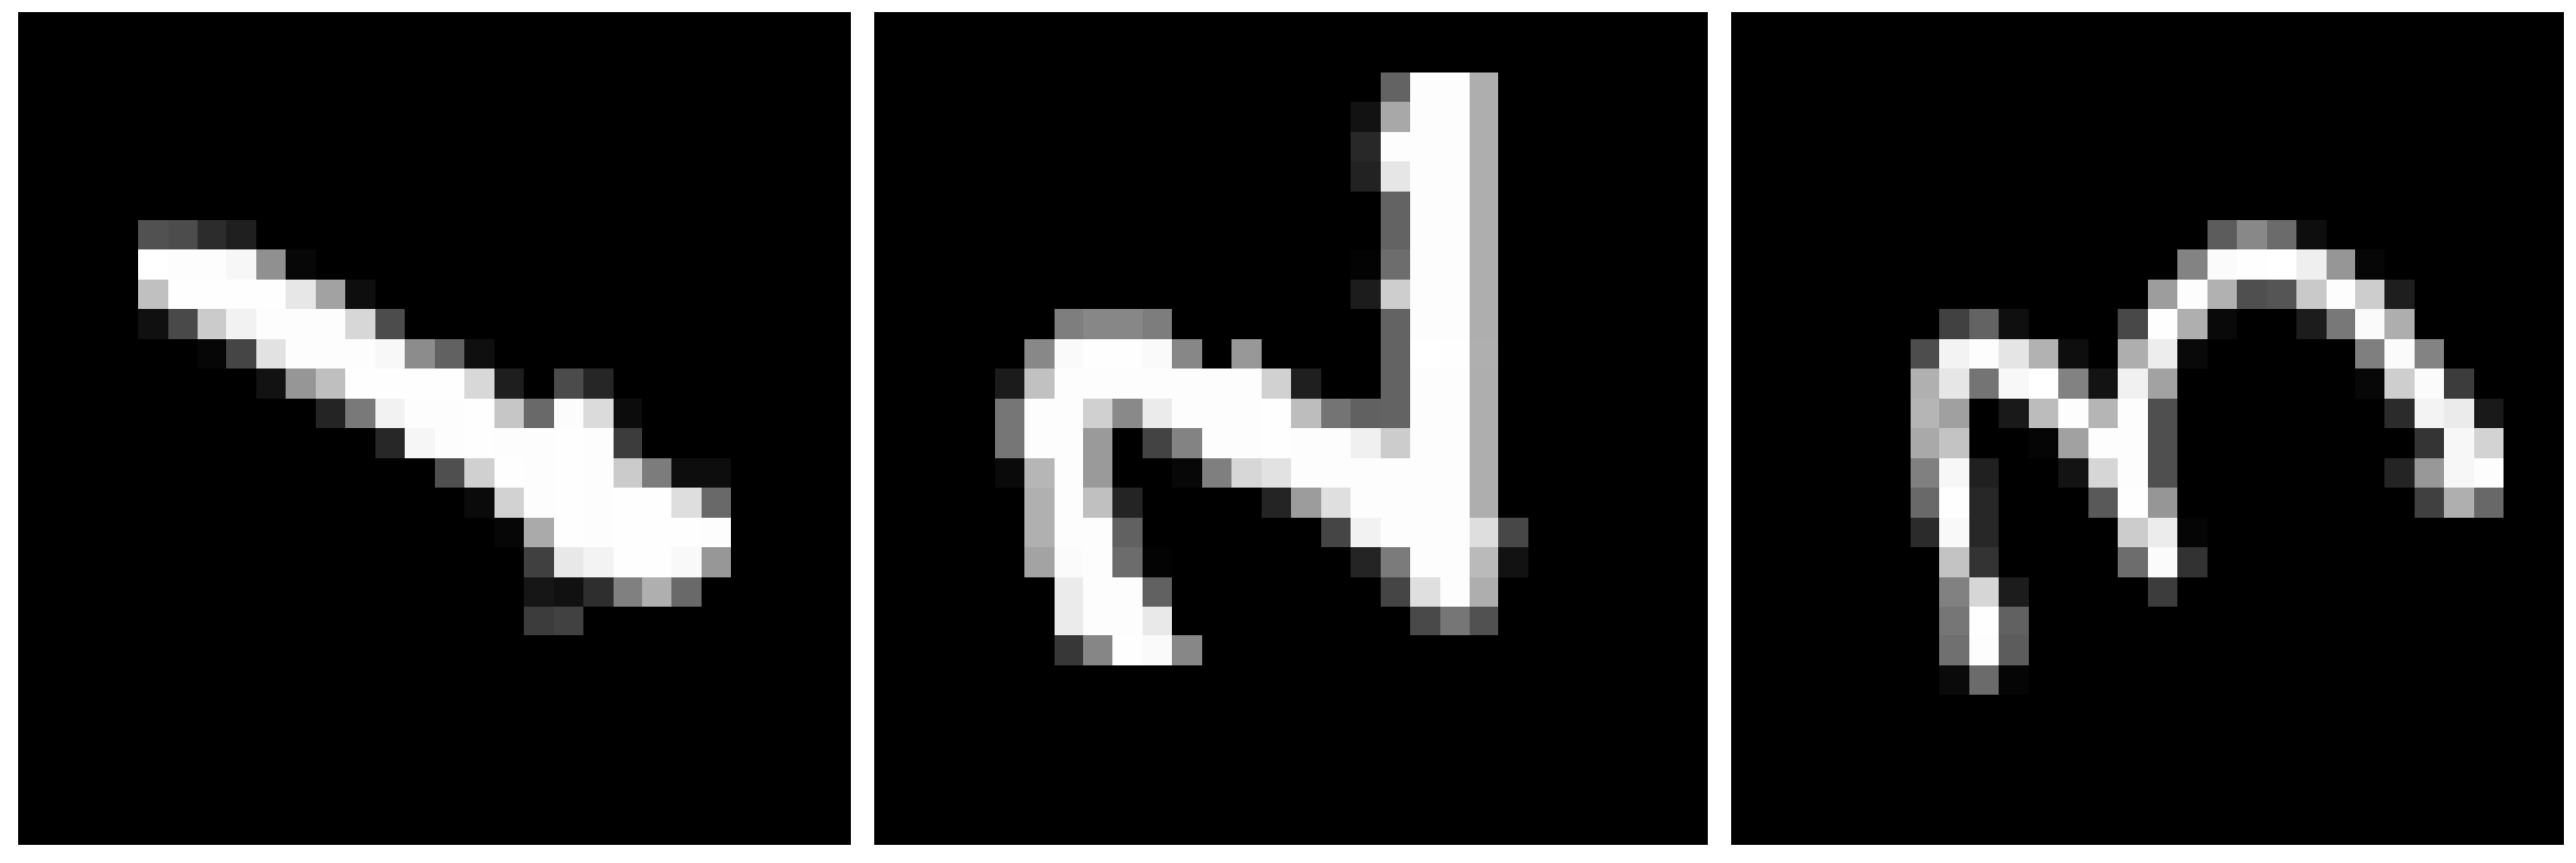
\includegraphics[width=0.3\linewidth]{figures/images/rmnist/rotation_90.pdf} \label{subfig:rmnist_images_90}}
  \caption{Visualization of example images from four domains of the Rotated MNIST dataset with rotation angles of $0^\circ$, $30^\circ$, $60^\circ$, $90^\circ$.}
  \label{fig:rmnist_images}
\end{figure}



\subsection{Experimental Configuration}
We evaluate each method on the multi-domain datasets via the leave-one-domain-out experiments,
% To do cross-domain experiments, we conducted the leave-one-domain-out evaluation, 
i.e., we train a model based on the source domains and test on the hold-out unseen target domain.
For example, when the target domain is $D_V$, then the transfer direction is from three source domains to a target domain, i.e., $D_L, D_C, D_S\rightarrow D_V$, and the average of test accuracies of four cross-domain experiments is taken as the final result.

We mainly consider the scenario when we have only limited labeled data from the source domains.
% , where robustness is expected to play an important role.
Therefore, for each domain, we randomly select some images to form the training set, validation set and test set for the cross-domain classification. 
The training set is used to learn robust models, whose
parameters are then selected on the validation set aggregated by the validation sets of each source domain.
The performance of a model is finally evaluated on the test set.
Details of the sets for training, validation and testing are as follows:
\begin{itemize}
    \item \textbf{Training set} For each domain, we randomly select up to $25$ images. To be more specific, we set the number of training images per category per domain to be a number in the set $\{2,3,5,7,10, 15, 20, 25\}$. 
    The training data from the three source domains form the training set.
    \item \textbf{Validation set} For each domain, $10$ images per category are randomly selected. The validation data from the three source domains form the validation set.
    \item \textbf{Test set} We sample $20$ images per category for each domain. The sampled test data from the unseen target domain form the test set.   
\end{itemize}
We repeat the above sampling process $5$ times for all datasets, so that the experiments are based on $5$ trials.The average results of all $5$ trials are finally reported.


Features pretrained on neural networks are taken as our input.
For the Rotated MNIST dataset, the Resnet-18 \cite{he2016deep} pretrained on the ImageNet is used to extract $512$-dimensional features as the inputs.
For the VLCS dataset, the pretrained $4096$-dimensional DeCAF features \cite{donahue2014decaf} are employed as the inputs of our algorithm following previous works \cite{motiian2017unified, dou2019domain}.
For the PACS dataset, we use the ImageNet pre-trained AlexNet \cite{krizhevsky2012imagenet} as the backbone network to extract the $9216$-dimensional features. 




% % ablation study figure, not used anymore
% \begin{figure*}
%   \centering
%   \subfloat[VLCS]
%     {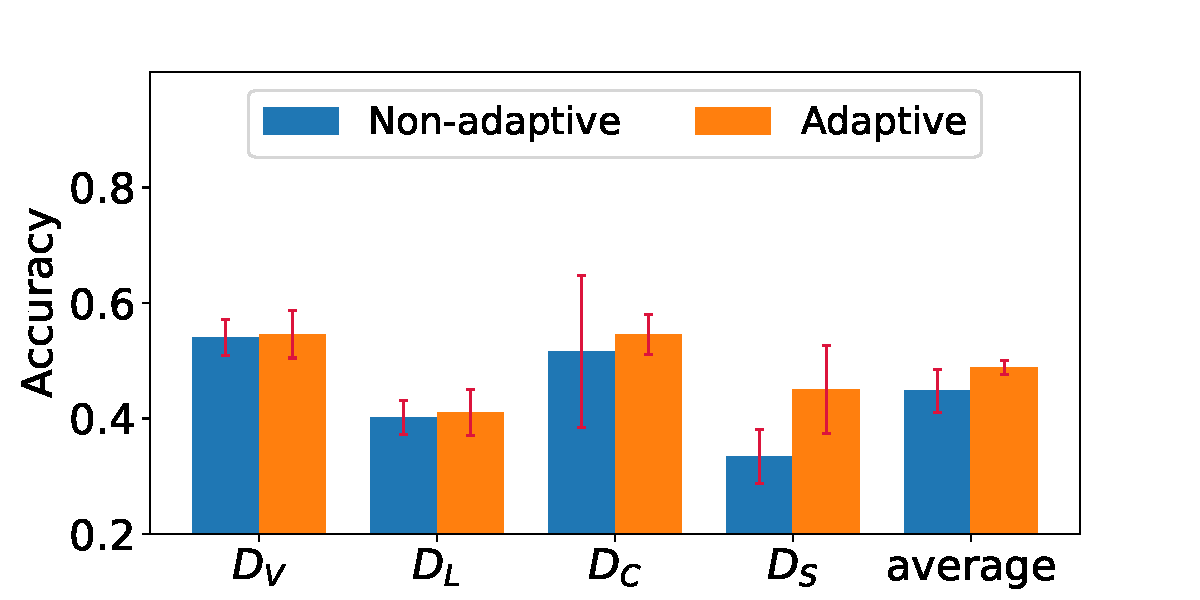
\includegraphics[width=0.3\linewidth]{figures/new_ablation/vlcs.pdf}\label{subfig:ablation_study_a}}
%     % \quad
%   \subfloat[PACS]
%     {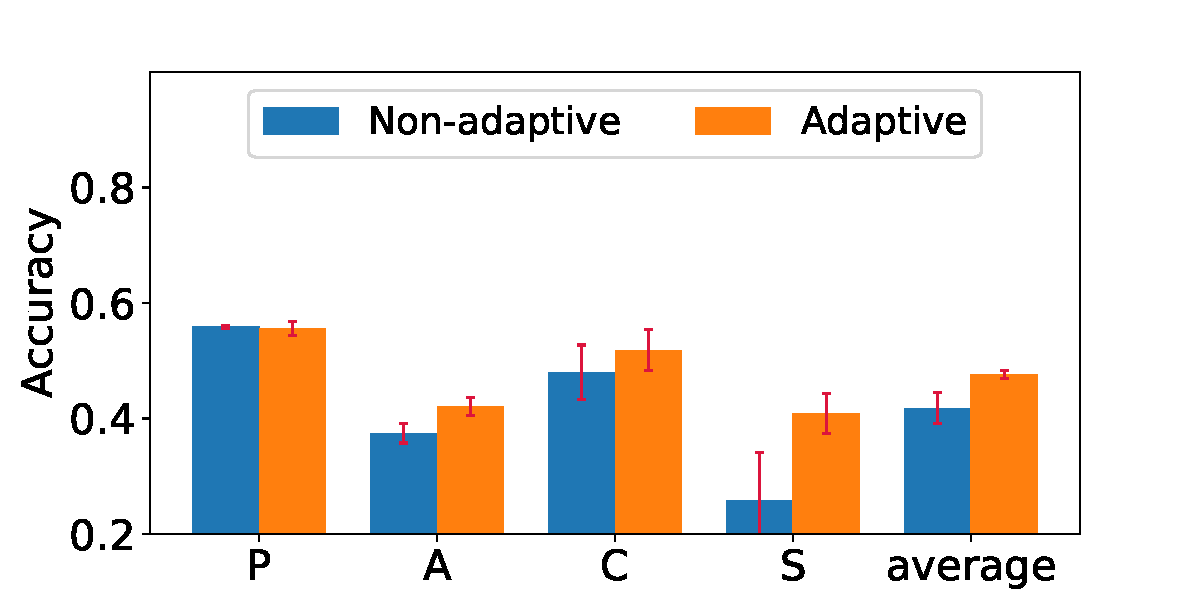
\includegraphics[width=0.3\linewidth]{figures/new_ablation/pacs.pdf}\label{subfig:ablation_study_b}}
% %   \quad 
%   \subfloat[Rotated MNIST]
%     {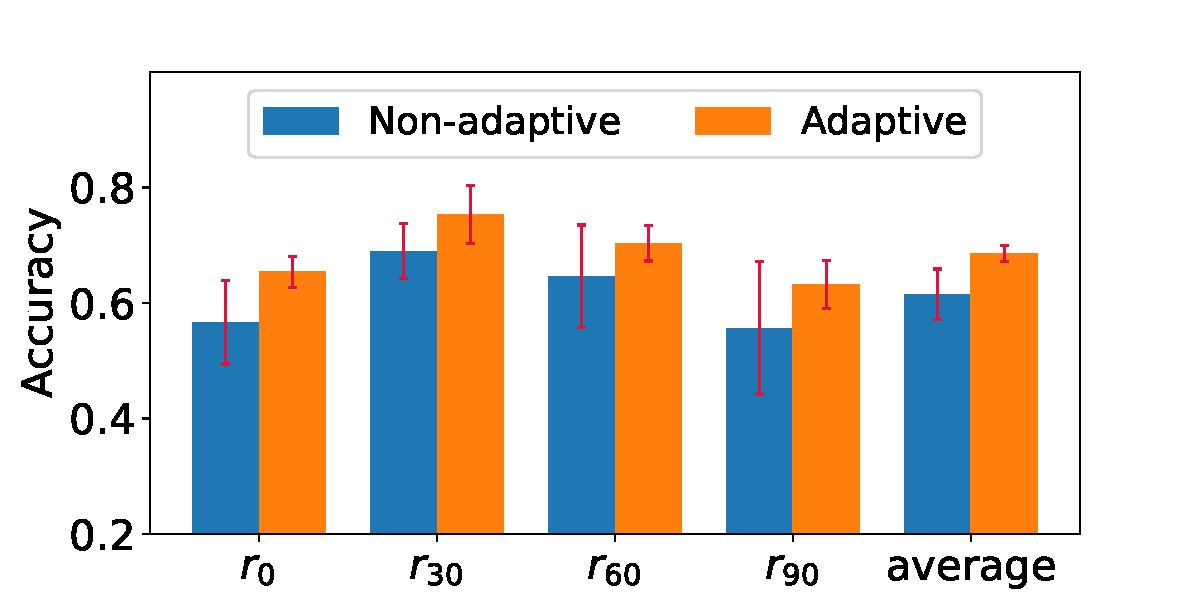
\includegraphics[width=0.3\linewidth]{figures/new_ablation/rmnist.pdf}\label{subfig:ablation_study_c}}
%   \caption{The effect of the optimal transport-based test-time domain adaptation for adaptive inference on the VLCS, PACS, and Rotated MNIST dataset.}
%   \label{fig:ablation_study}
% \end{figure*}

\subsection{Baseline Methods}
We compare our proposed WDRDG framework with the following baseline methods in terms of the average classification accuracy.
All methods for comparison are summarized as below:
\begin{itemize}
    \item {KNN:} We adopt the combination of training instances from all source domains to train the nearest neighbor classifier.
    \item {MDA \cite{hu2020domain}:} We apply Multidomain Discriminant Analysis (MDA) to learn domain-invariant feature transformation
    % is a domain generalization method 
    that is applicable when $P(X|Y)$ changes across domains.
    1-NN is adopted as a classifier to the learned feature transformations for classification.
    \item {CIDG \cite{li2018domain2}:} Conditional Invariant Domain Generalization (CIDG) finds a linear transformation to minimize the total domain scatter with regard to each class-conditional distributions. The learned features are also classified using KNN.
    \item {MLDG \cite{li2018learning}}: We consider this meta-learning based domain generalization method as another baseline which models unseen target domain shift. 
    A simple two-layer network is trained to learn the classifier.
    % \item {WDRDG.} Our framework
    
    % Further adding the optimal-transport based adaptive inference in Section leads to our overall framework.
\end{itemize}

% We first compare our proposed DRO based domain generalization method with the simple baseline, KNN, which uses the combination of training instances from all source domains to train a nearest neighbor classifier. 
% We also compare our method with domain generalization methods that also explicitly considers the class-conditional shift on ${P}(X|Y)$, i.e., MDA  \cite{hu2020domain} CIDG \cite{li2018domain2}, and MLDG \cite{li2018learning} which is a meta-learning training strategy for domain generalization.
For our proposed WDRDG framework, 
% the parameter of the size of uncertainty radius is determined via validation.
% Also, we determine the neighborhood size of the KNN classifier via validation.
% in our implementation of Algorithm \ref{algorithm},
we use the CVXPY package \cite{diamond2016cvxpy} to solve the distributionally robust optimization problem.
% (\ref{eq:add_wass_all}). 
The Wasserstein distance of order 2 is used for all experiments, and calculated with the POT package \cite{flamary2021pot}. 


\subsection{Results and Discussion}
% results for each target domain
\begin{figure*}[!t]%[H]
  \centering
%   \subfloat[PASCAL VOC2007]
  {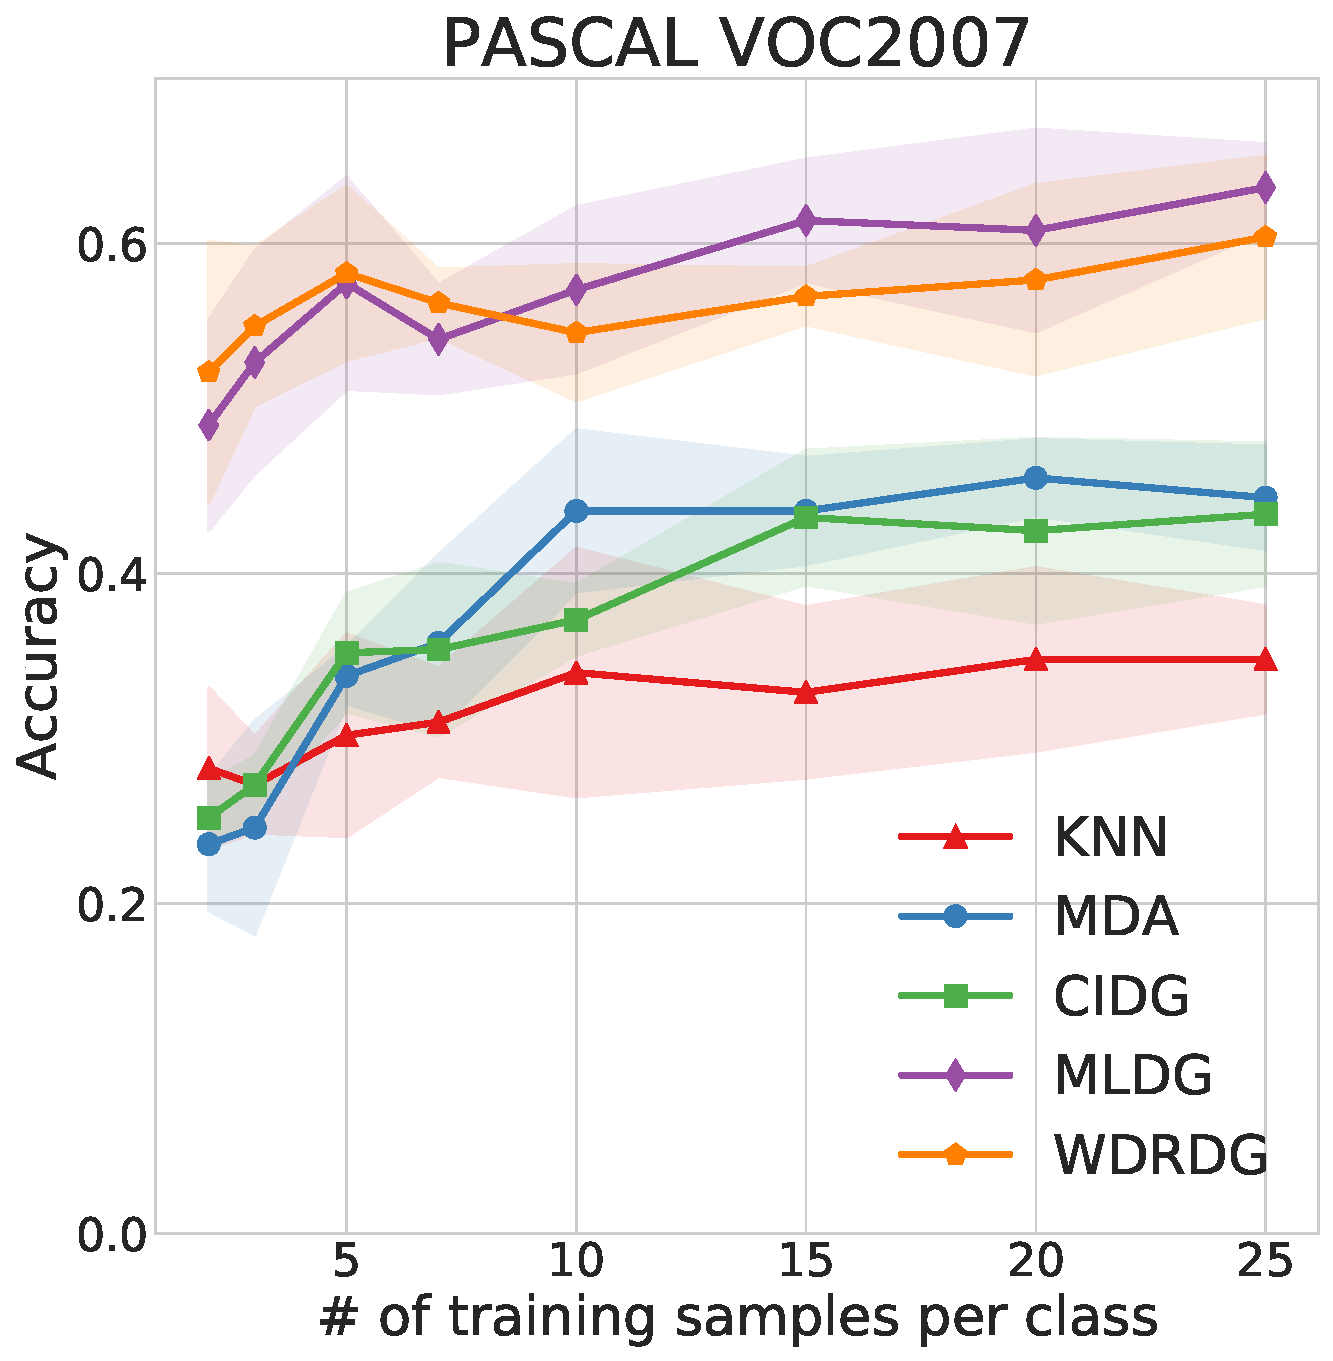
\includegraphics[width=0.23\linewidth]{figures/results/vlcs/V.pdf}\label{subfig:vlcs_results_V}}
%   \subfloat[LabelMe]
  {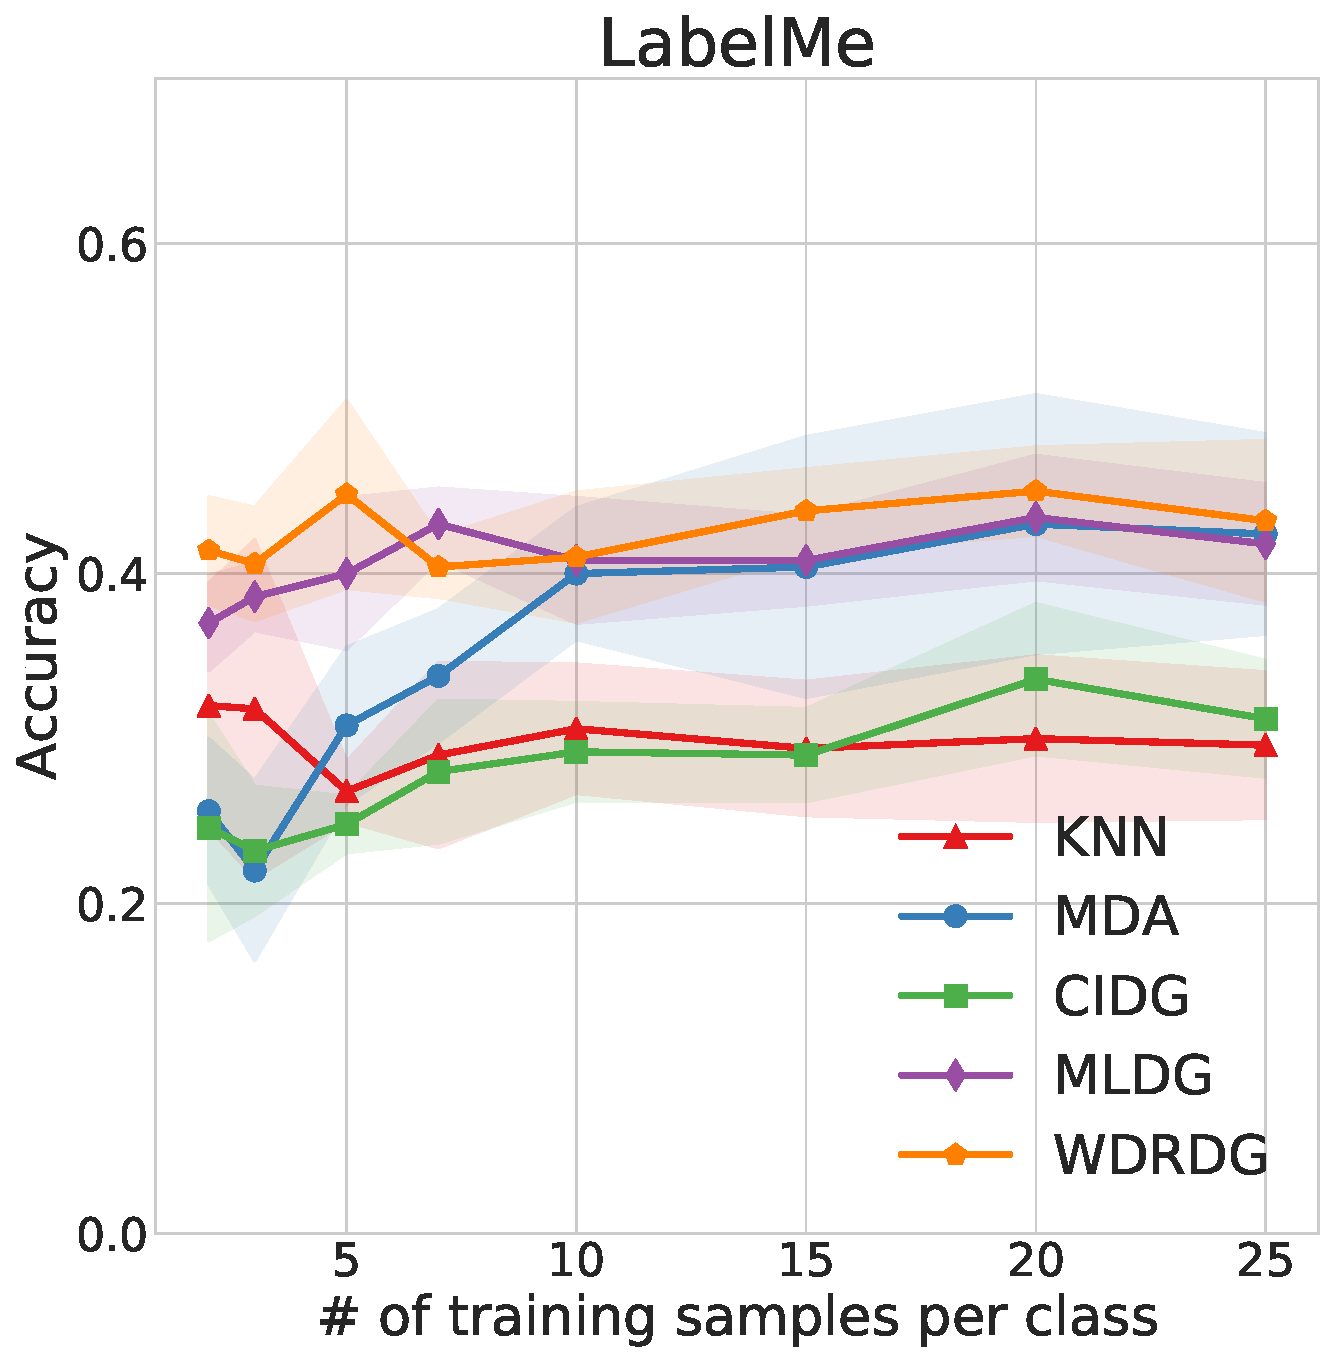
\includegraphics[width=0.23\linewidth]{figures/results/vlcs/L.pdf}\label{subfig:vlcs_results_L}}
%   \subfloat[Caltech-101]
  {
\includegraphics[width=0.23\linewidth]{figures/results/vlcs/C.pdf}\label{subfig:vlcs_results_C}}
%   \subfloat[SUN09]
  {
\includegraphics[width=0.23\linewidth]{figures/results/vlcs/S.pdf}\label{subfig:vlcs_results_S}}
  \quad 
%   \subfloat[Photos]
  {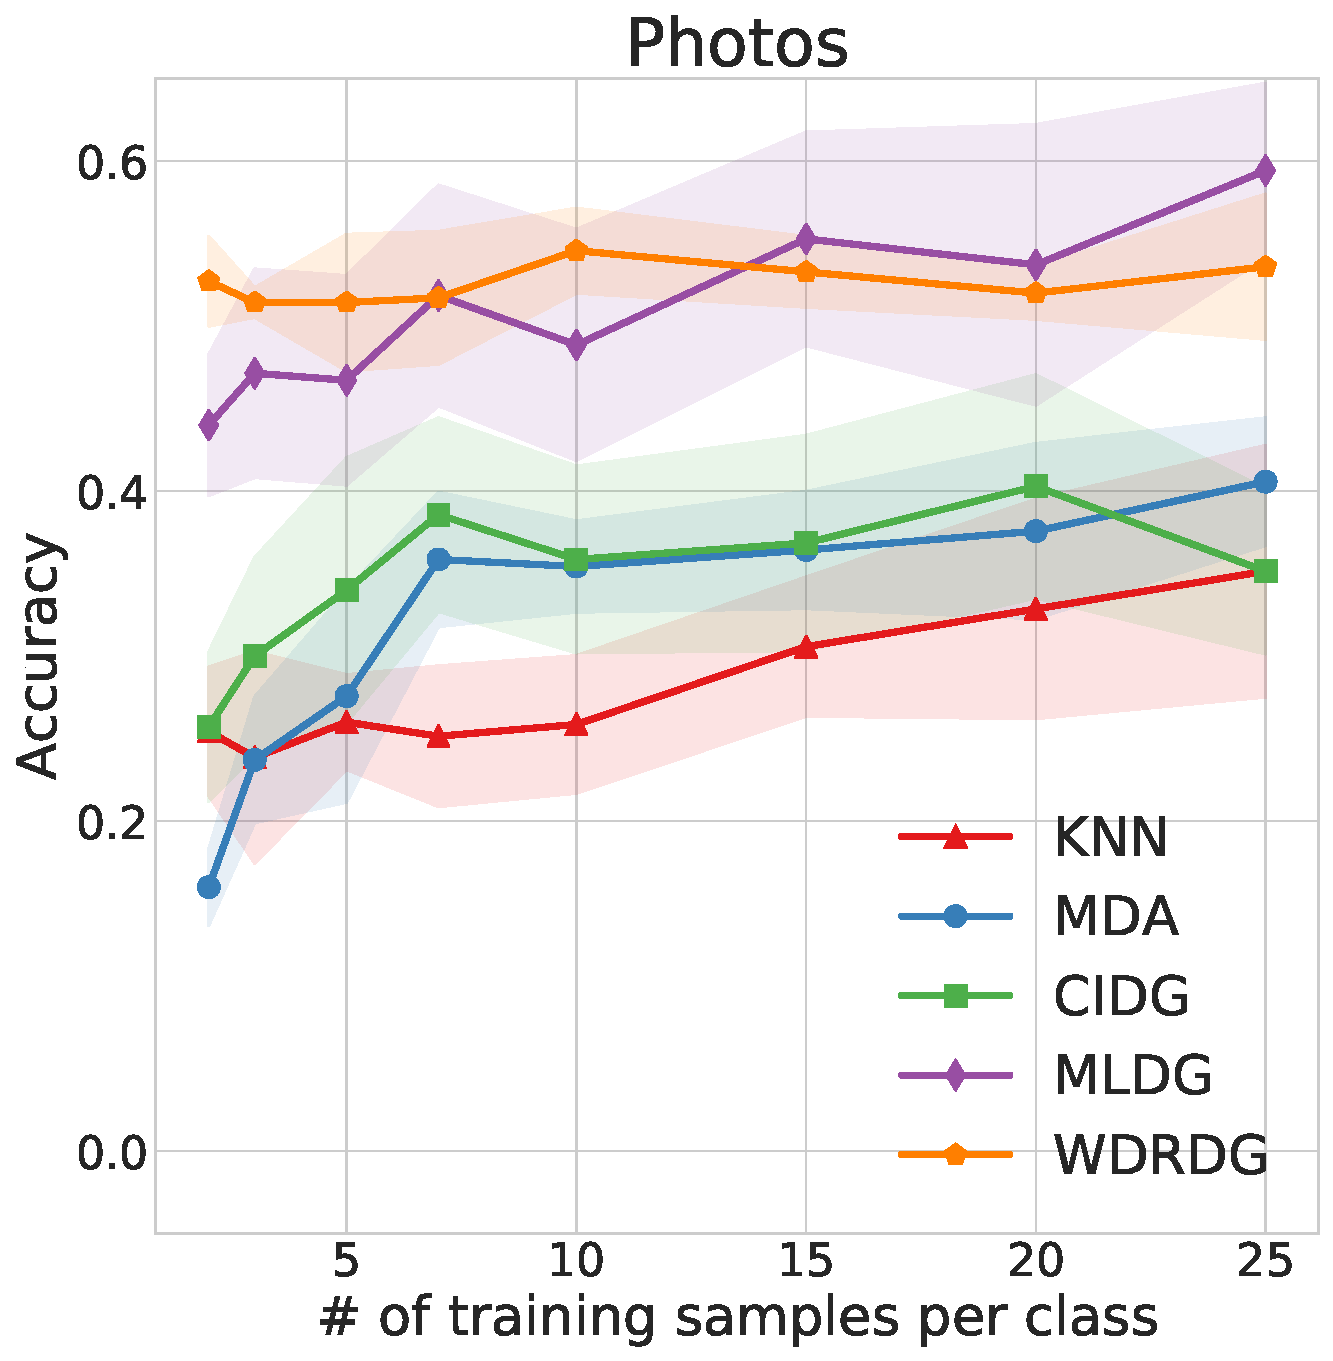
\includegraphics[width=0.23\linewidth]{figures/results/pacs_results/P.pdf}\label{subfig:pacs_results_P}}
%   \subfloat[Art Painting]
  {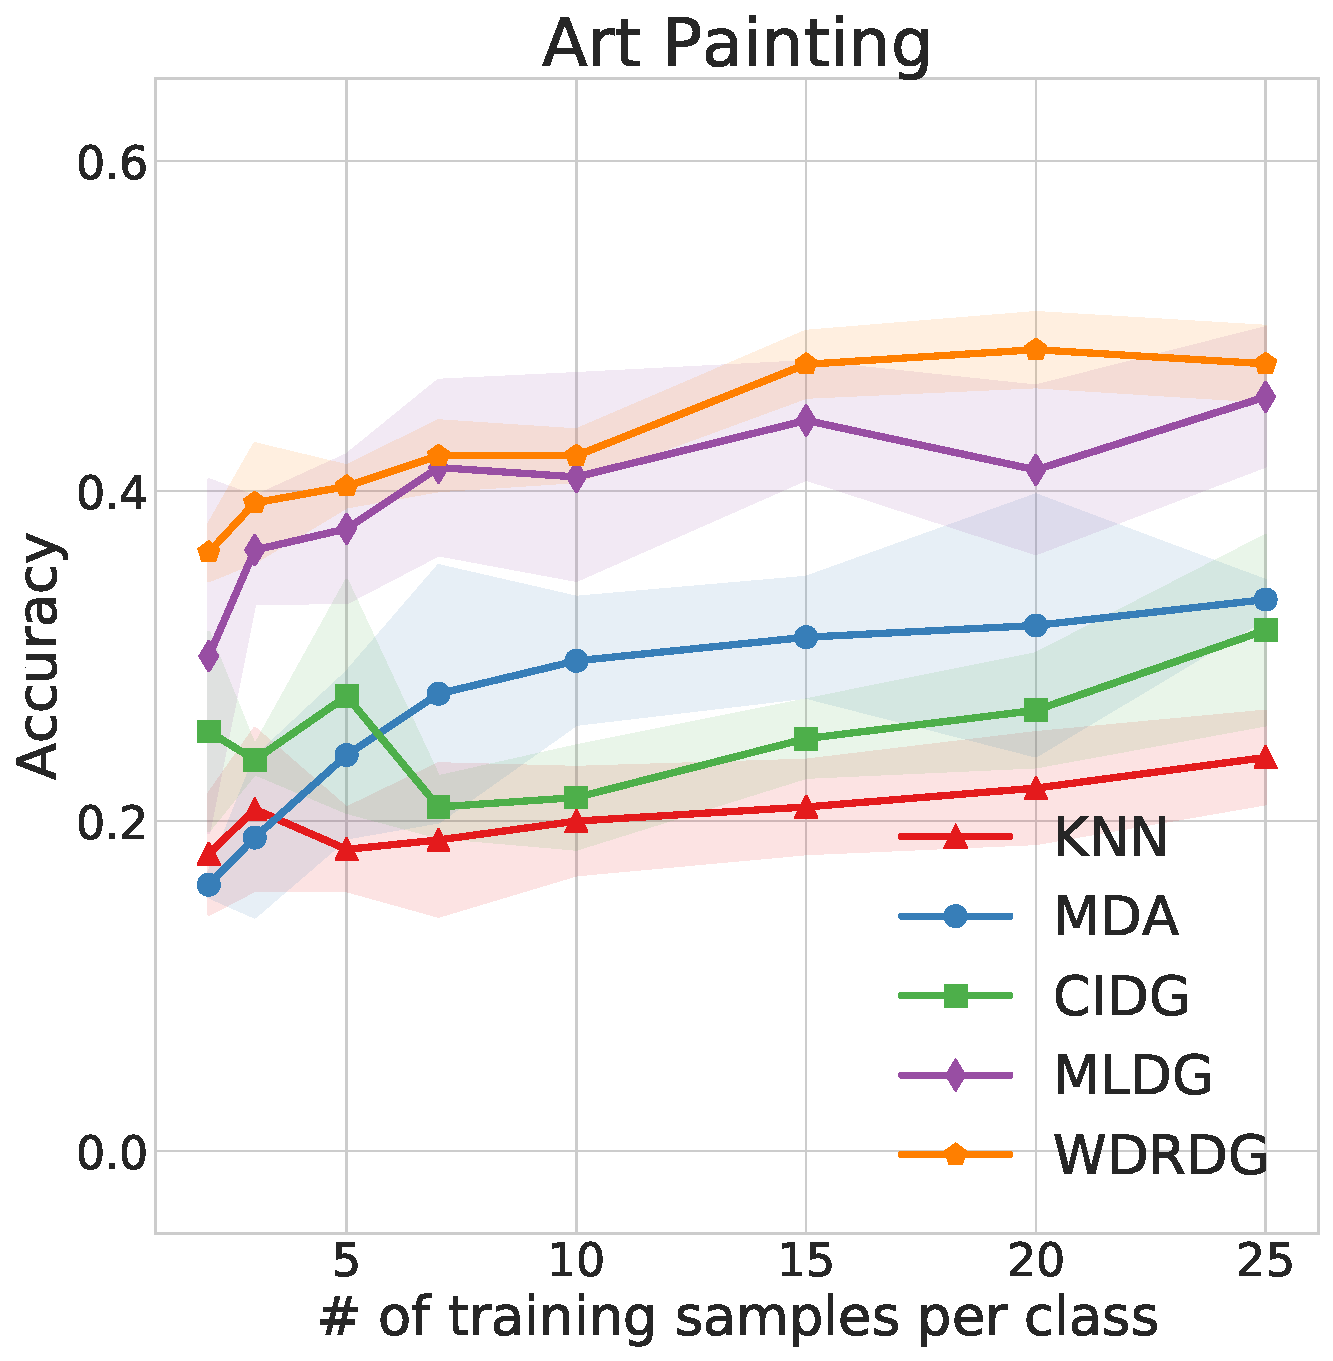
\includegraphics[width=0.23\linewidth]{figures/results/pacs_results/A.pdf}\label{subfig:pacs_results_A}}
%   \subfloat[Cartoon]
  {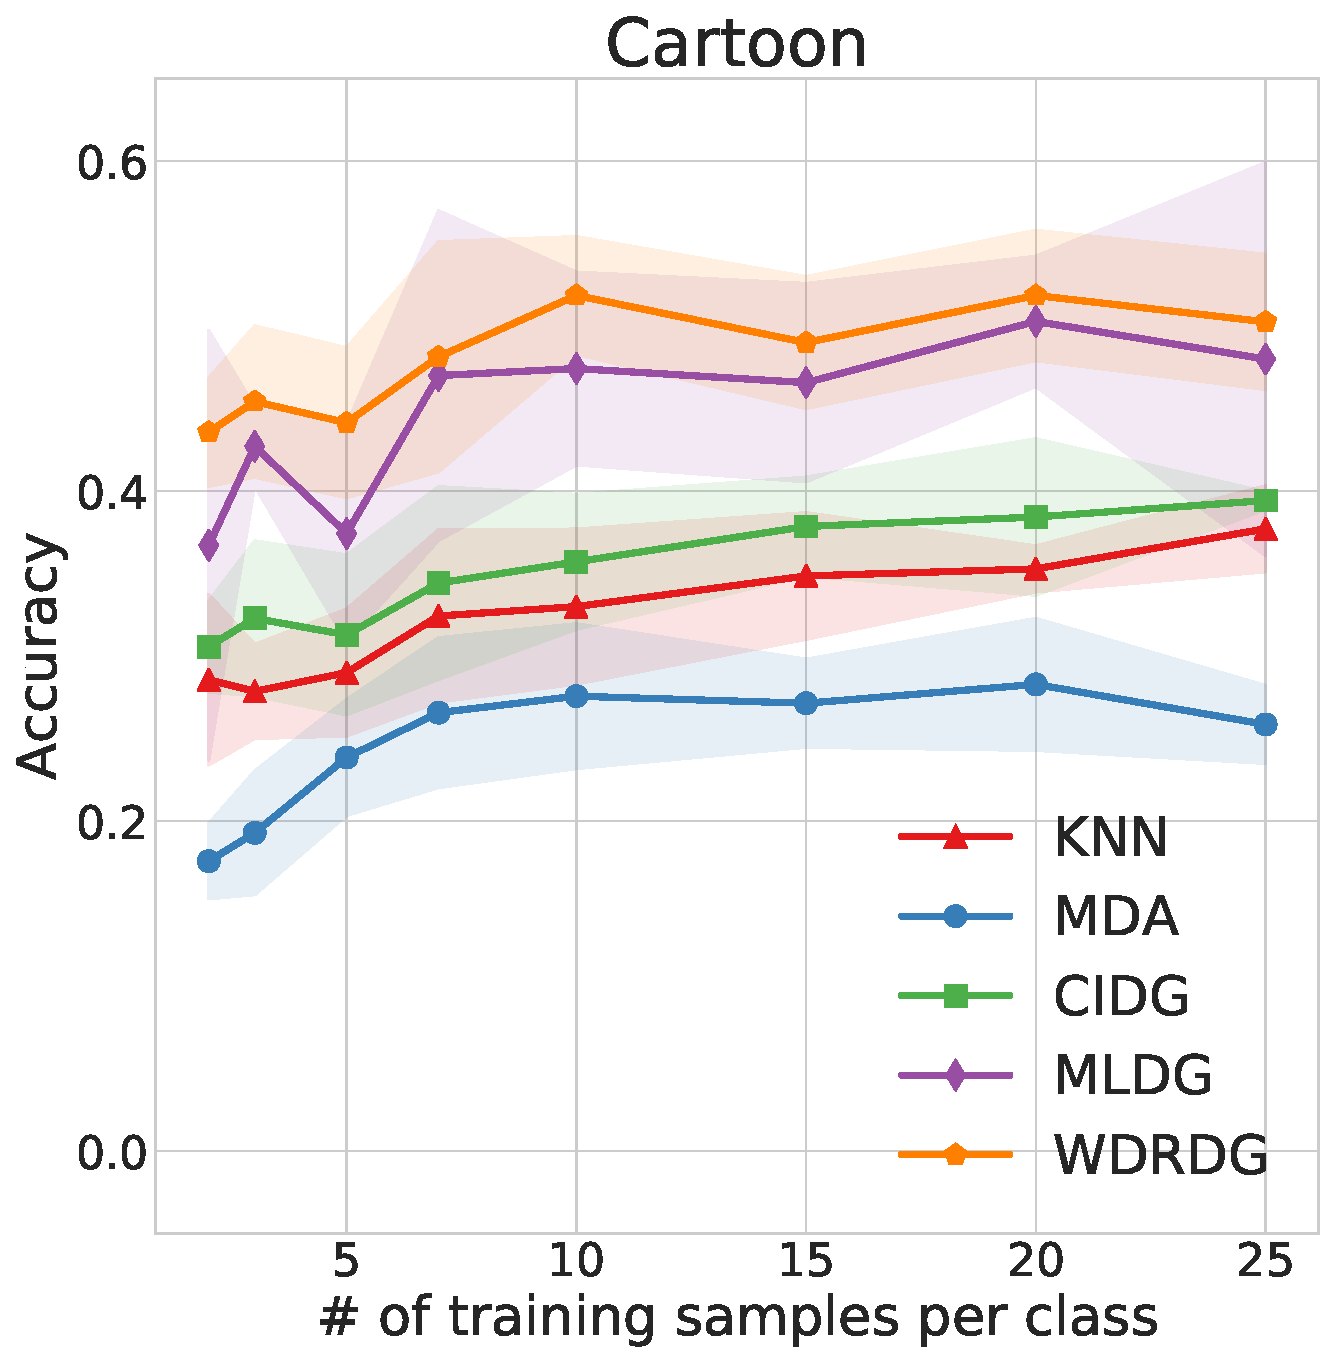
\includegraphics[width=0.23\linewidth]{figures/results/pacs_results/C.pdf}\label{subfig:pacs_results_C}}
%   \subfloat[Sketch]
  {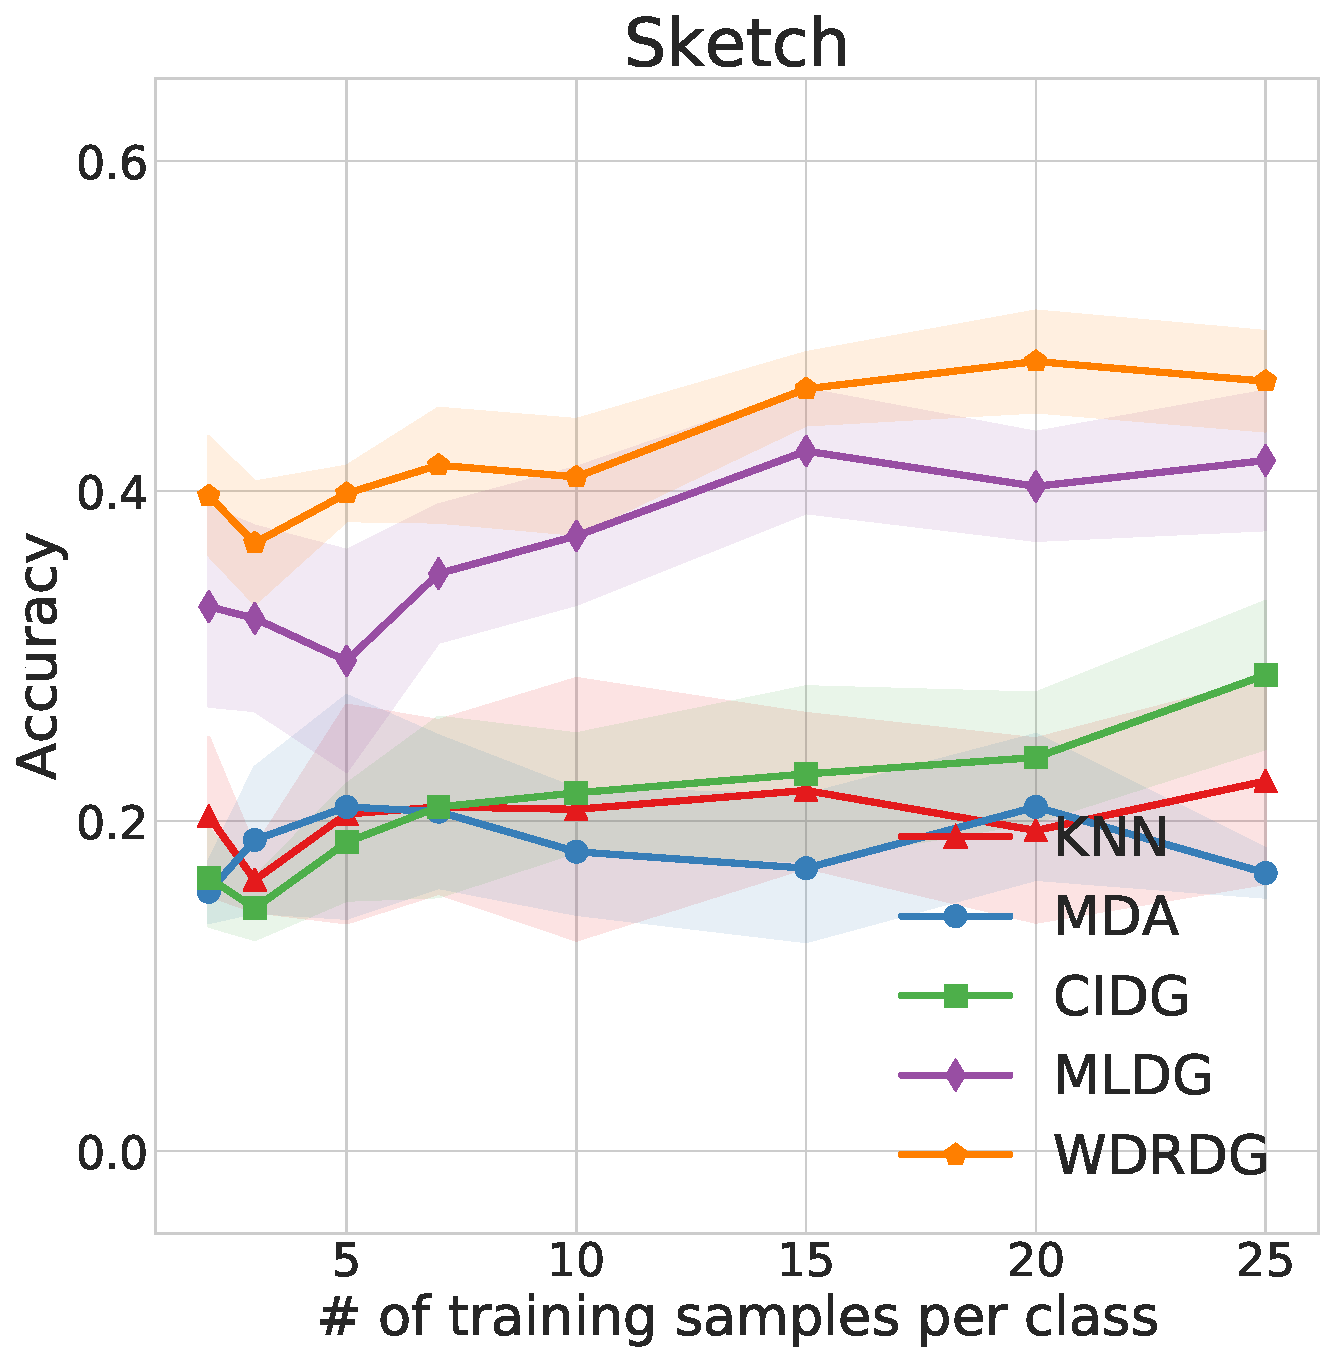
\includegraphics[width=0.23\linewidth]{figures/results/pacs_results/S.pdf}\label{subfig:pacs_results_S}}
  \quad 
%   \subfloat[$r_0$]
  {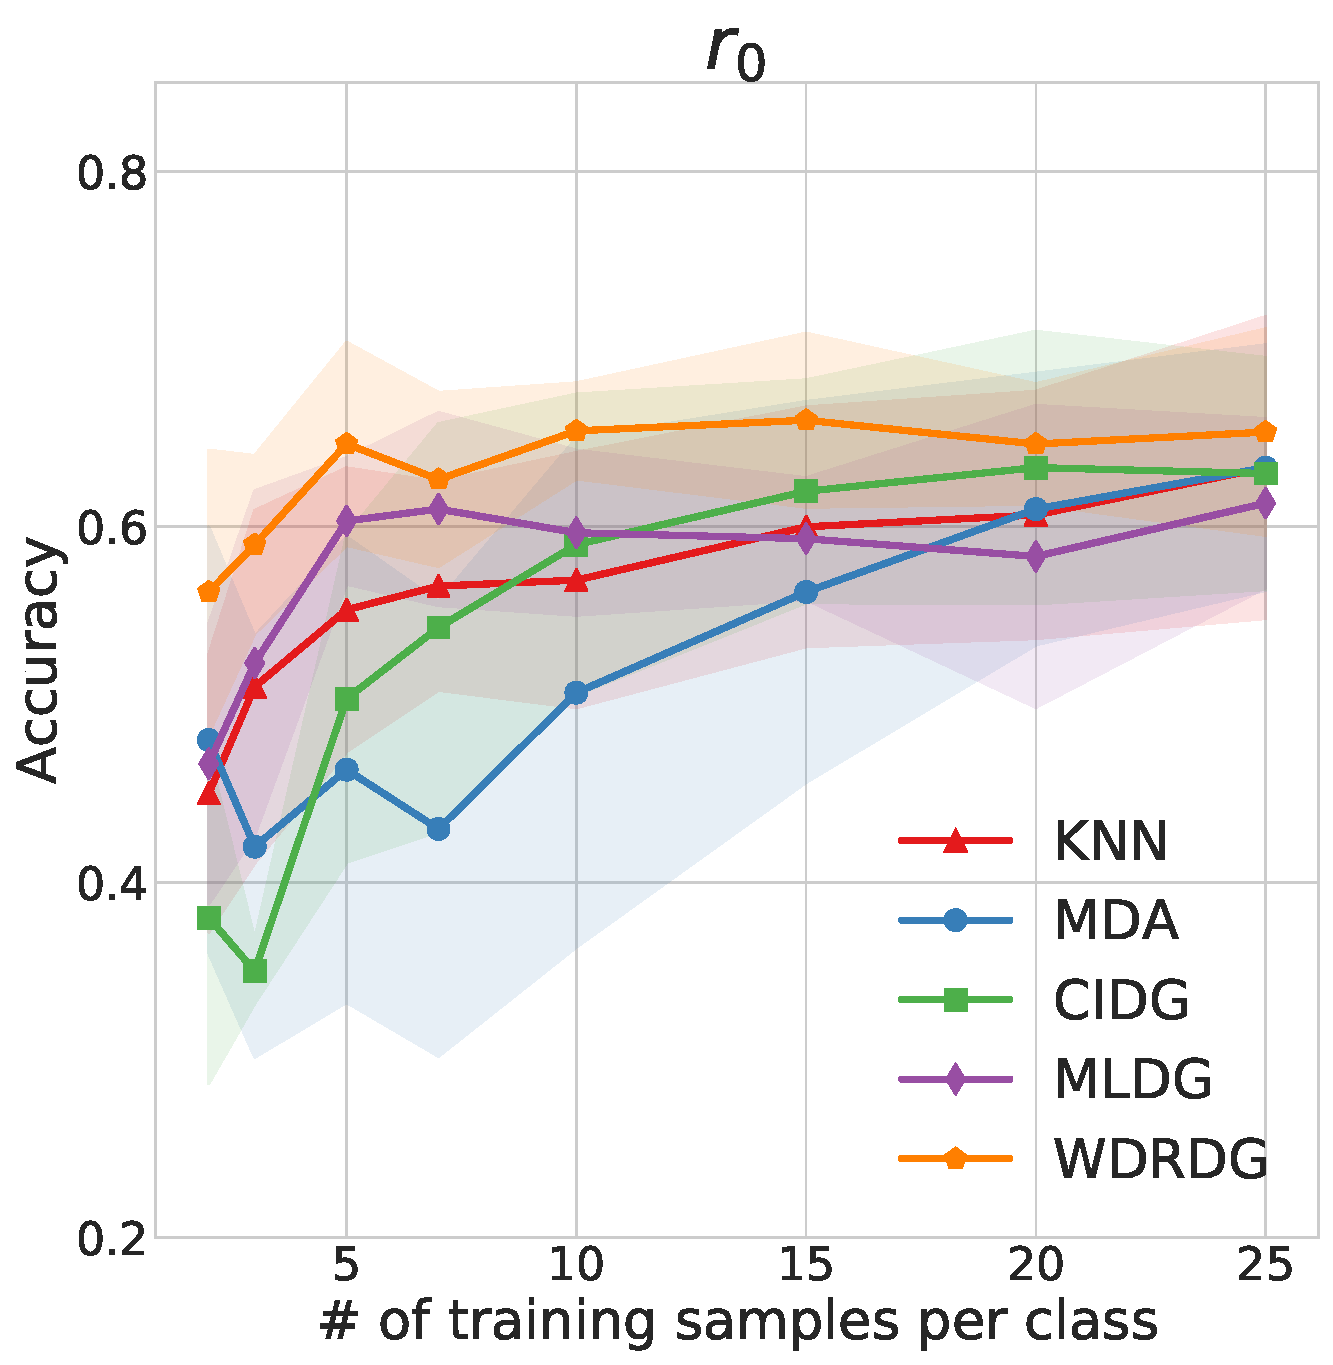
\includegraphics[width=0.23\linewidth]{figures/results/rmnist_results/r_0.pdf}  \label{fig:rmnist_results_0}}
%   \subfloat[$r_{30}$]
  {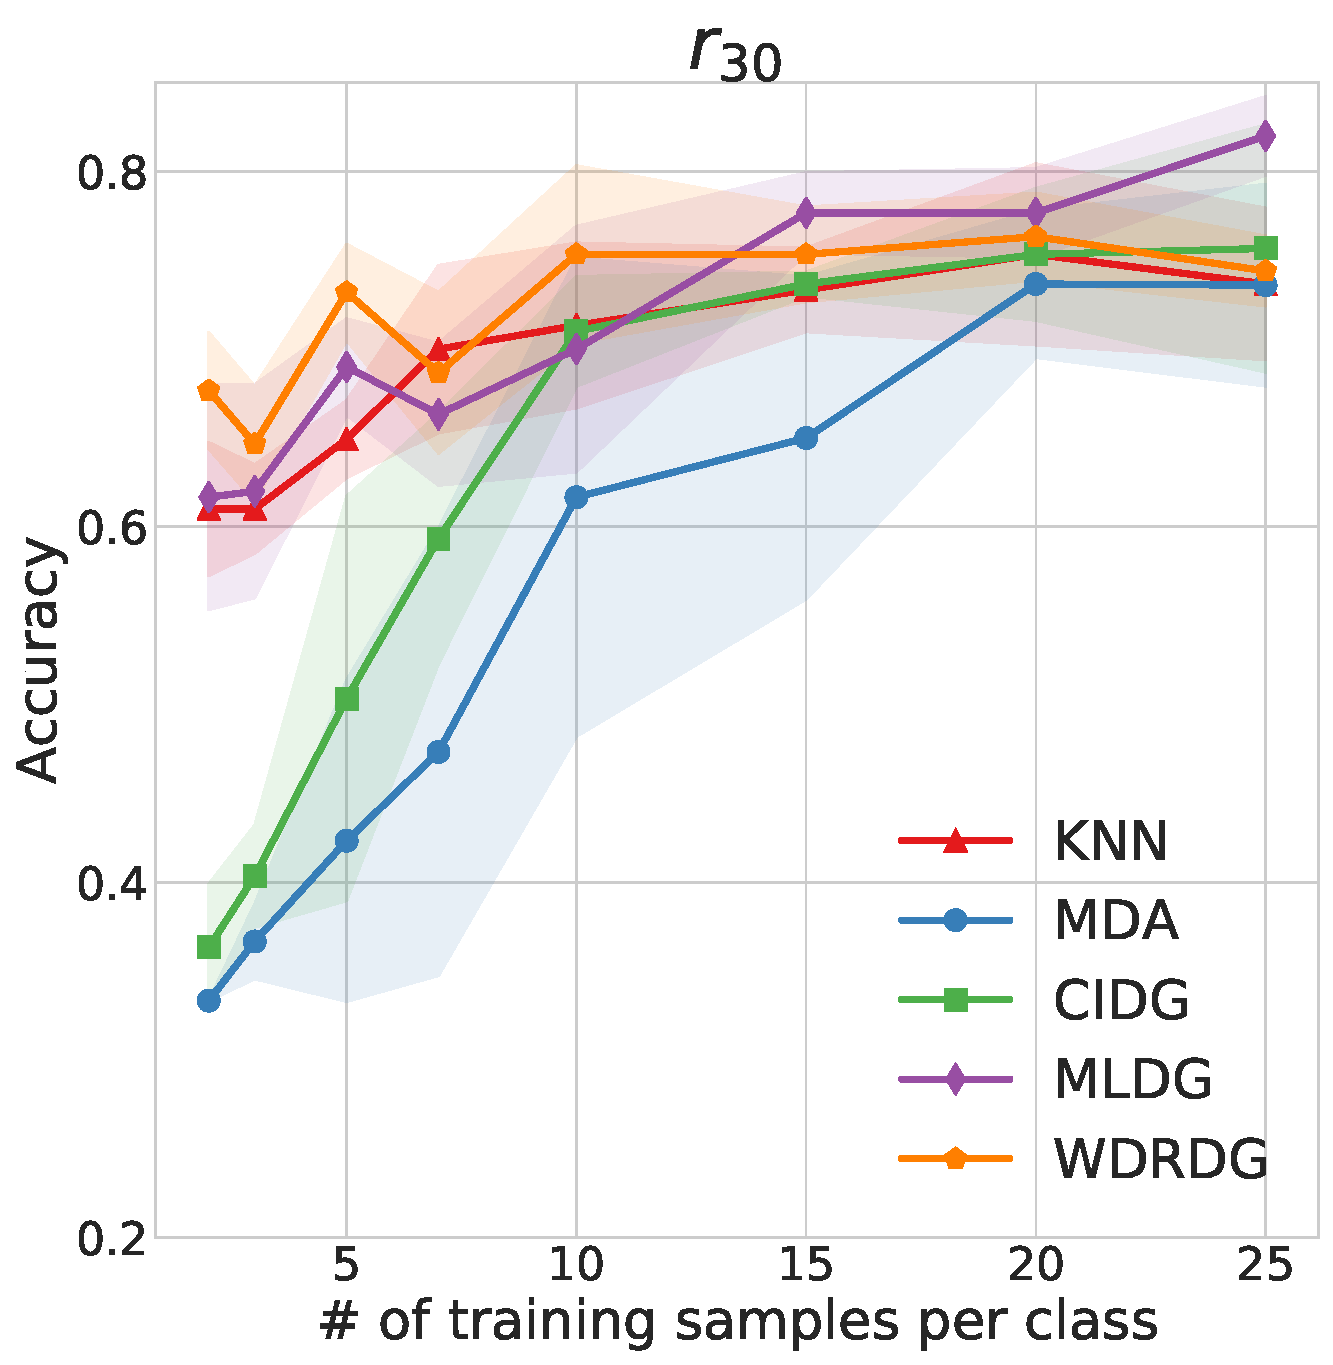
\includegraphics[width=0.23\linewidth]{figures/results/rmnist_results/r_30.pdf}\label{fig:rmnist_results_30}}
%   \subfloat[$r_{60}$]
  {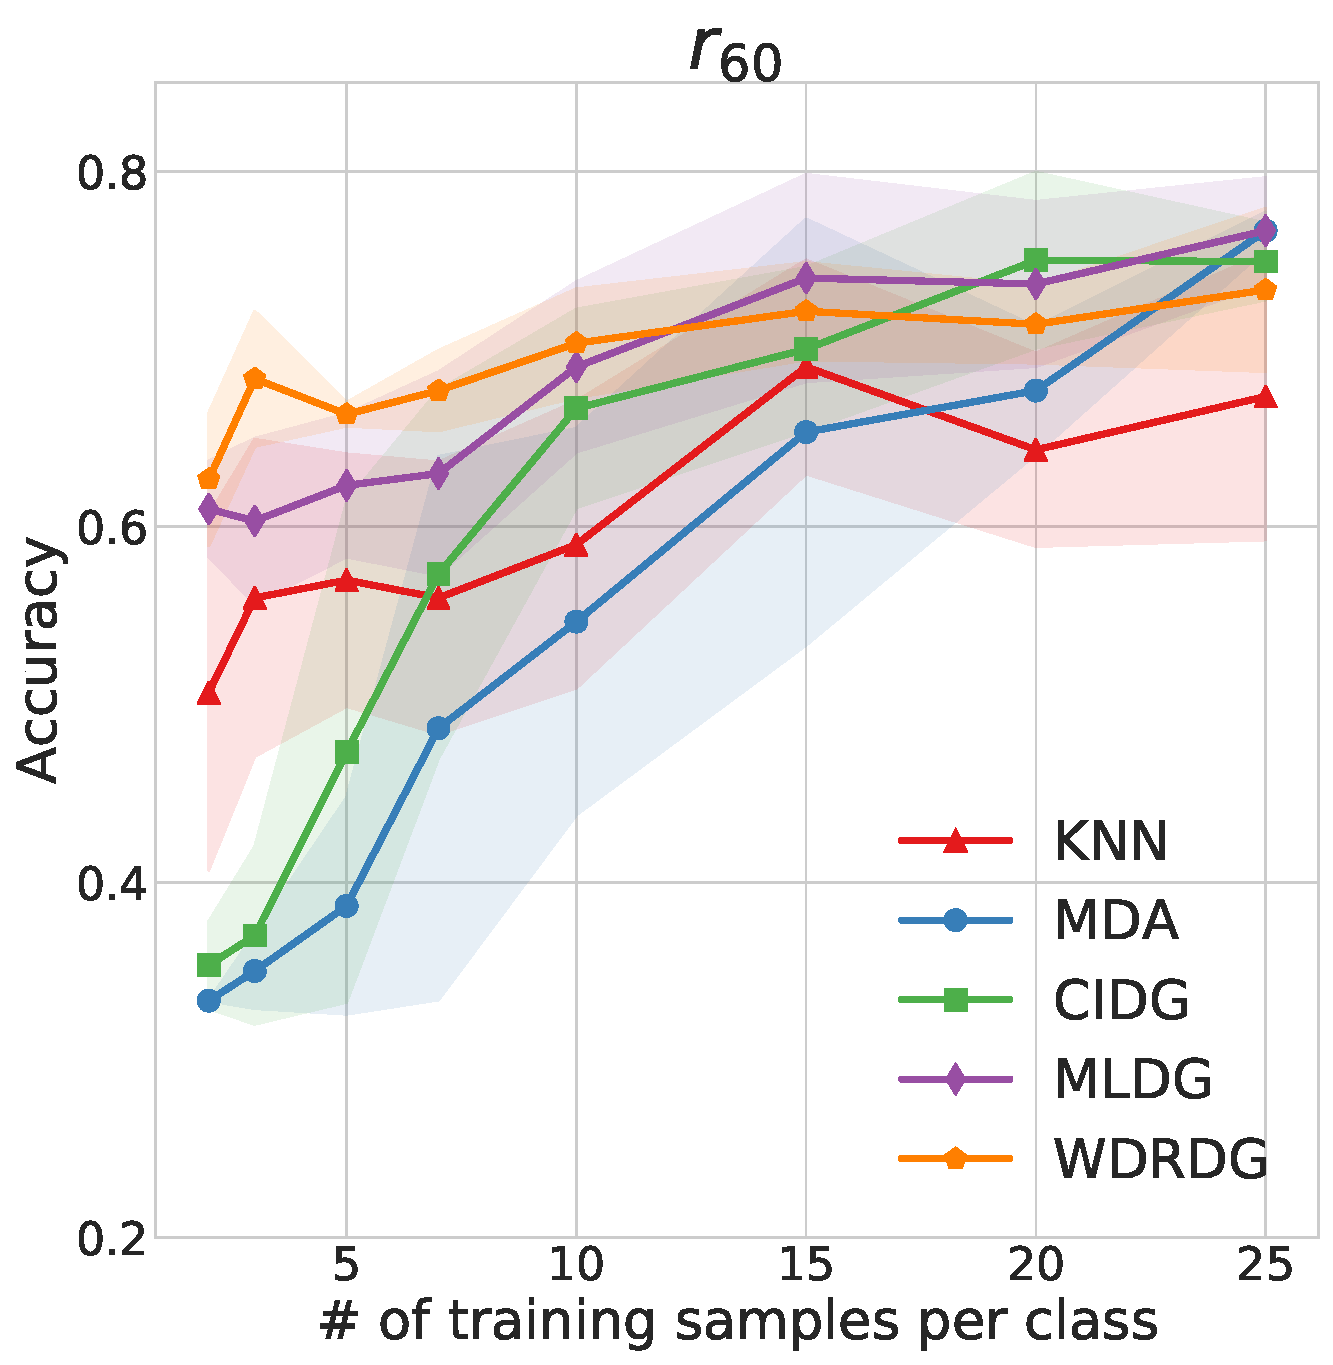
\includegraphics[width=0.23\linewidth]{figures/results/rmnist_results/r_60.pdf}\label{fig:rmnist_results_60}}
%   \subfloat[$r_{90}$]
  {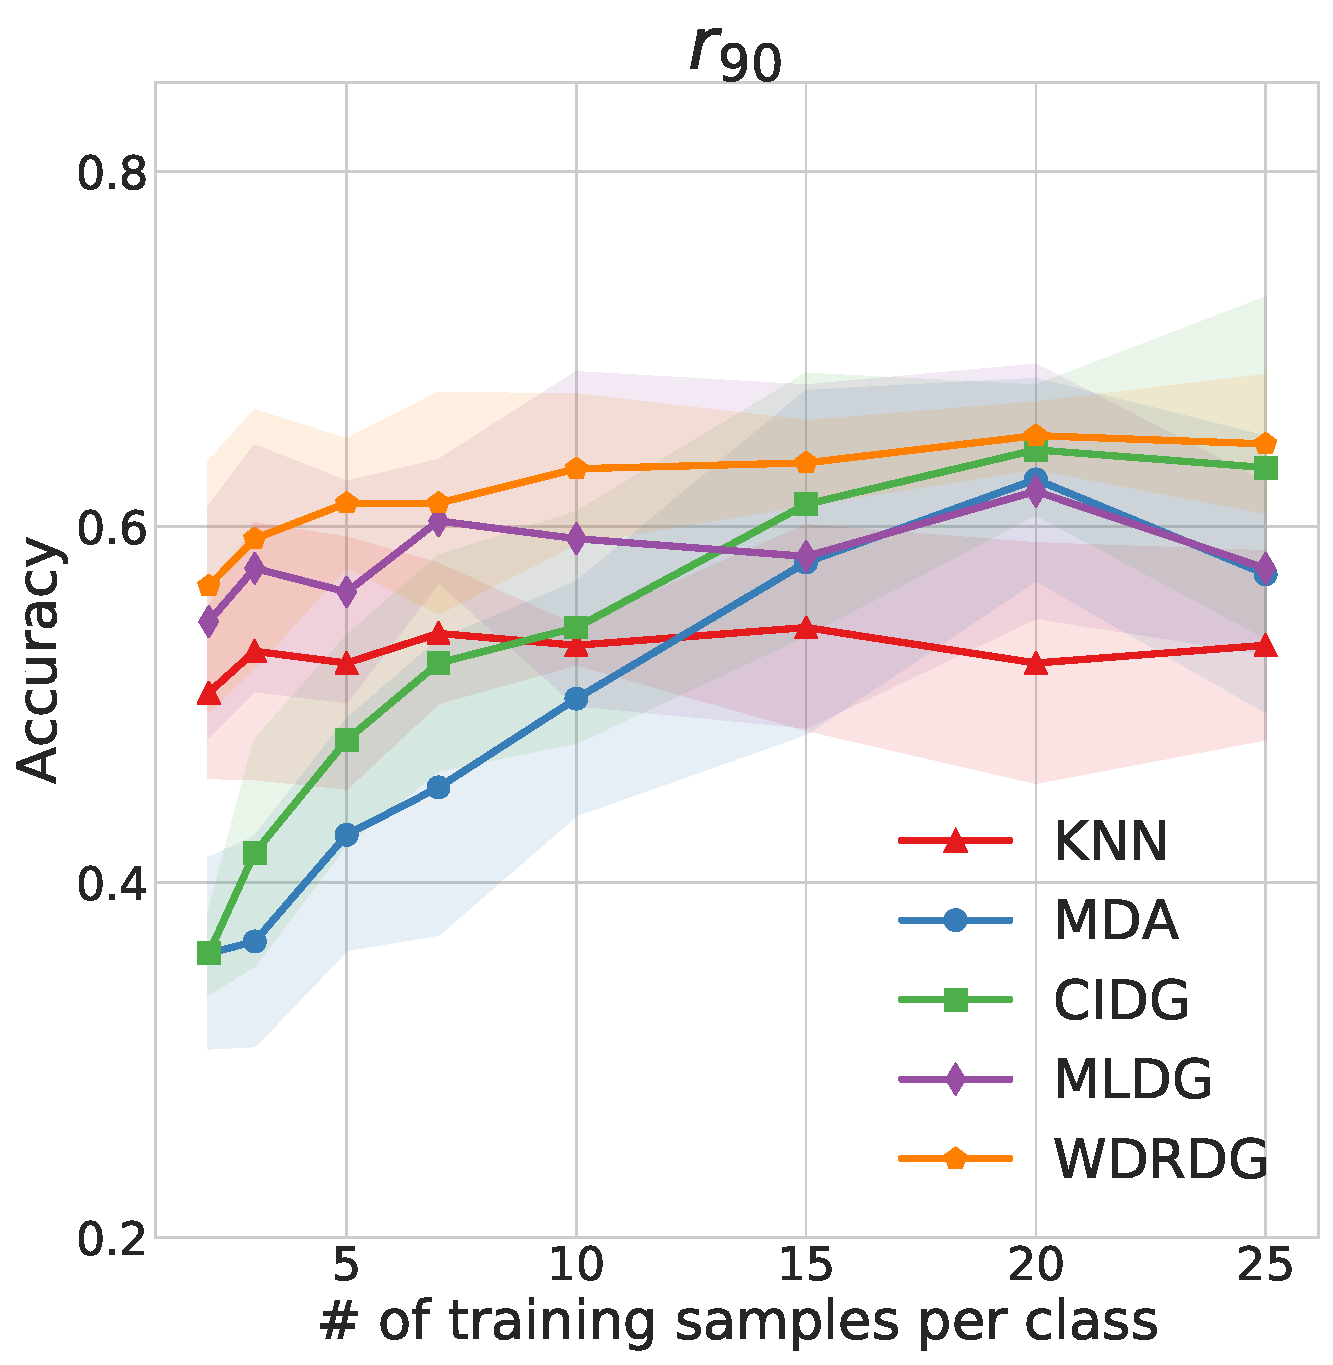
\includegraphics[width=0.23\linewidth]{figures/results/rmnist_results/r_90.pdf}\label{fig:rmnist_results_90}}
\caption{Performance comparison for the VLCS, PACS and Rotated MNIST dataset under different size of training samples per class. Each row shows the results for a dataset, and each column shows the generalization result for a certain target domain. Average performance of five methods are represented by different colors, and the corresponding shadow shows the standard deviation of 5 experimental trials. 
Our WDRDG framework outperforms KNN, MDA and CIDG with higher accuracy and smaller standard deviation.
% Also, it has more advantage especially when the source training sample size is limited.
Also, it has more advantage over MLDG especially when the source training sample size is limited. For example, WDRDG outperforms MLDG by up to 
$46.79\%$ when the target domain is Caltech-101 in the VLCS dataset, by up to $20.95\%$ for target domain Art Painting in the PACS dataset, 
and by up to  $20.71\%$ for target domain $r_{0}$ in the Rotated MNIST dataset  with training sample size of 2 for each class.
}
\label{fig:all_results}
\end{figure*}

% average results
\begin{figure*}
    \centering
  \subfloat[VLCS]{
\includegraphics[width=0.26\linewidth]{figures/results/vlcs/average.pdf}\label{subfig:vlcs_ave}}
  \subfloat[PACS]{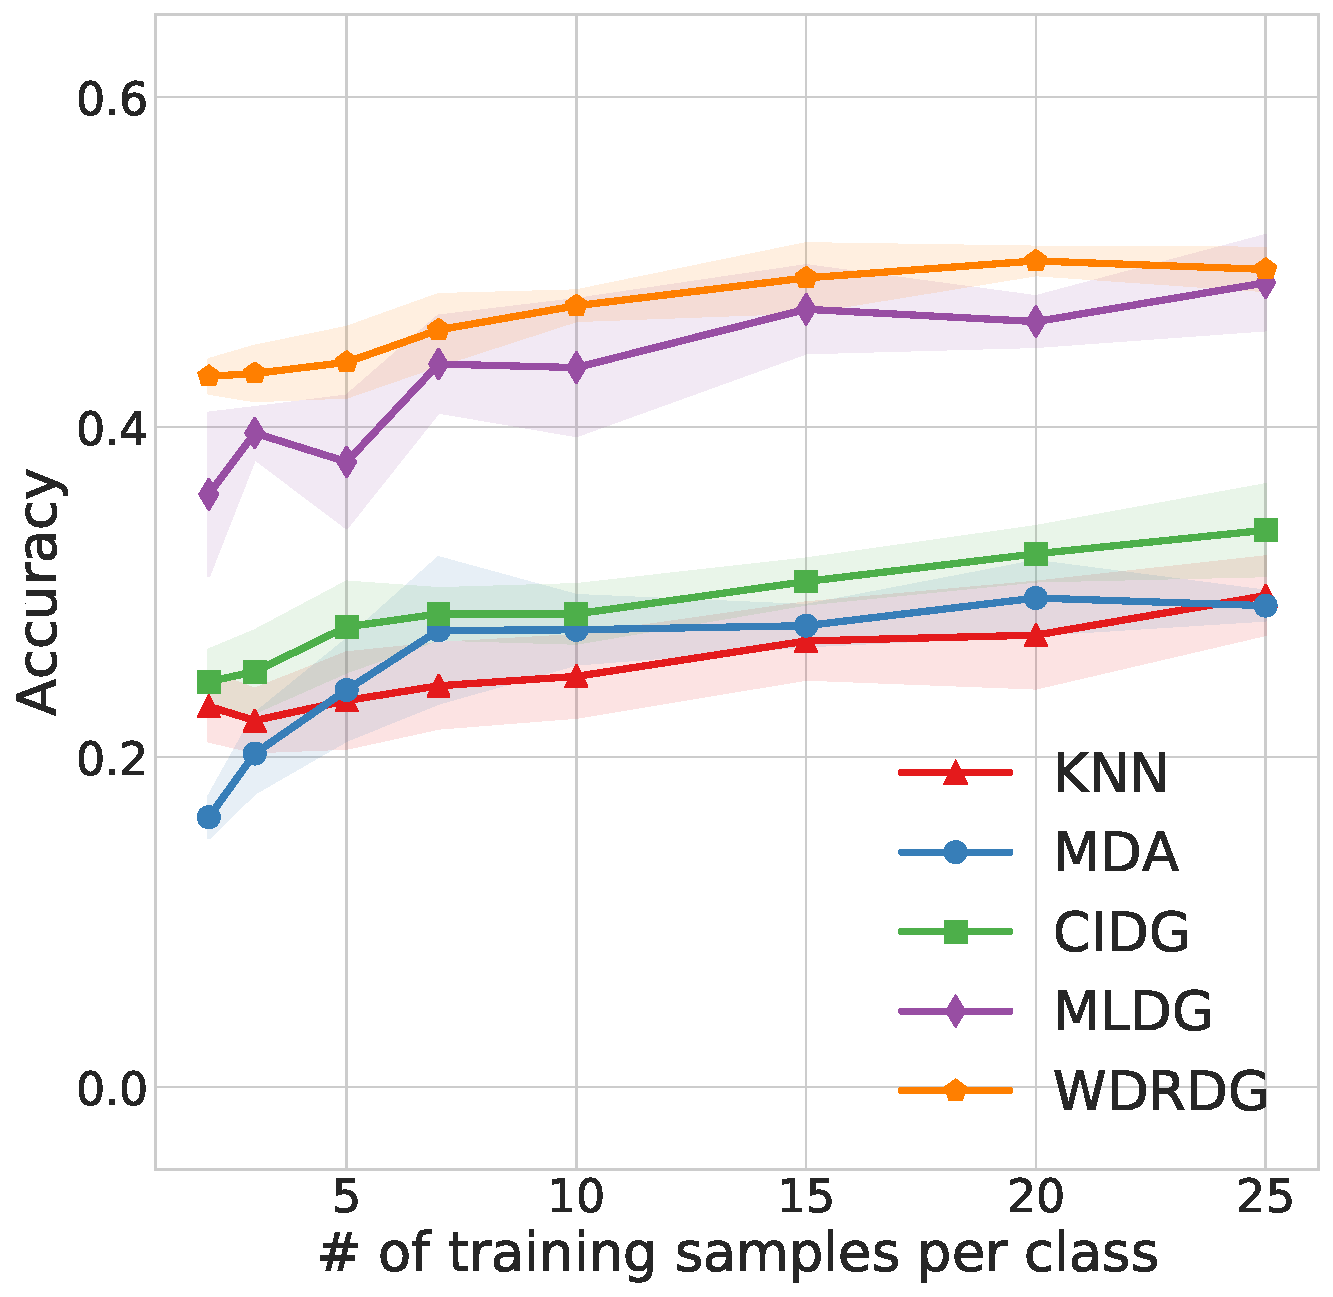
\includegraphics[width=0.26\linewidth]{figures/results/pacs_results/average.pdf}\label{subfig:pacs_ave}}
  \subfloat[Rotated MNIST]{
\includegraphics[width=0.26\linewidth]{figures/results/rmnist_results/average.pdf}\label{subfig:rmnist_ave}}
    \caption{Average generalization performance of different methods on the VLCS, PACS and Rotated MNIST dataset. As the training sample size increases, all methods obtain better performance. Our WDRDG framework outperforms other baselines, especially in few-shot settings. When the sample size is less than 10 per class, WDRDG provides at least $3.75\%$, $4.73\%$, $3.86\%$ better generalization ability than others on the VLCS, PACS and Rotated MNIST dataset, respectively.}
    \label{fig:results_ave}
\end{figure*}


% We compare the performance on the VLCS dataset of our proposed framework with other methods. 
% Different methods are compared by the average classification accuracy over $5$ trials for each choice of target domain. 
In this section, we present the results for domain generalization on all three datasets.
When each domain serves as the target domain, the results are shown in Figure \ref{fig:all_results}, with the plotted lines representing the average performance over $5$ trials and the shaded area representing the corresponding standard deviation.

For the VLCS dataset, we report the results in the first row in Figure \ref{fig:all_results}.
In all four cases when each domain serves as the unseen target domain, our method achieves better classification accuracy and standard deviation than other methods when the training sample size for each class is very few, i.e., 2, 3 or 5. 
The advantage over MLDG then levels off as the sample size reaches to over 10 per class.
The performance improvement against MLDG reaches as high as $6.53\%$, $11.89\%$, $46.79\%$, $22.54\%$ with only 2 training samples for each class when the target domain is PASCAL VOC2007, LabelMe, Caltech-101 and SUN09, respectively, which confirms that our method is efficient for few-shot cases.
% When the target domain is PASCAL VLC2007 or Caltech-101, WDRDG underperforms MLDG as the sample size reaches to over 10 per class,
% this shows that our framework 
% this shows that the  deep-learning methods may make better use of the extracted deep features via fine-tuning.


The second row of Figure \ref{fig:all_results} reports the classification accuracy results for the PACS dataset.
The proposed WDRDG achieves the best results in accuracy and standard deviation when the target domain is Art Painting, Cartoon, or Sketch using different training sample size, and MLDG outperforms WDRDG when the target domain is Photos with the sample size 15 for each class. 
WDRDG outperforms MLDG by up to $19.81\%$, $20.95\%$, $18.68\%$, $20.35\%$ for each target domain when the training sample size is 2. 
This validates the effect of our method when the training sample size is limited. 
The improvement of WDRDG over other methods on the PACS dataset is relatively larger compared with the improvements on the VLCS dataset. This improvement is especially obvious over MDA and CIDG when the target domain is Sketch, shown in the fourth column of the second row in Figure \ref{fig:all_results}.
This may because that the differences among domains are greater in PACS where the image styles are obviously different compared with in VLCS, where samples from different domains are real-world images collected from different perspectives or scales. This demonstrates that our WDRDG could better handle scenarios with larger unseen domain shift. 



The results for the Rotated MNIST dataset in the third row of  Figure \ref{fig:all_results} also yield similar conclusions. As the training sample size increases, almost all methods converges to the same accuracy for different target domain.
% However, when the target domain is $r_{90}$, 
When the training sample size is smaller, i.e., the training sample per class for each source domain is $2,3,5,7$, the advantage of  our proposed framework is more obvious. 
WDRDG outperforms MLDG by $20.71\%$, $9.73\%$, $2.73\%$, $3.66\%$ when the training sample size is 2 for each class for target domain $r_{0}$, $r_{30}$, $r_{60}$, and $r_{90}$, respectively.
When the training sample size is big, e.g., the training sample per class for each source domain is $25$, even simple KNN method performs well. 
% as shown in the first column in the third row in Figure \ref{fig:all_results}.
% When the target domain is $r_{30}$ or $r_{60}$ which are the relative easier generalization cases compared with target domain $r_{0}$ or $r_{90}$, WDRDG has less obvious advantages. 
This is consistent with the analysis in the above two datasets. 


Figure \ref{fig:results_ave} reports the average performance of different target domains on the three datasets.
Overall, our method is the most stable under different numbers of training samples, with narrower shadow band of standard deviation.
% especially compared with MLDG, whose standard deviation is larger compared with WDRDG in most cases with different number of training samples.
As the size of training samples gets bigger, all methods have the tendency of performing better.
On the PACS and Rotated MNIST dataset, WDRDG achieves the best average performance under different training sample size compared with other methods.
On the VLCS dataset, WDRDG also achieves pretty good accuracies with smaller standard deviation.
In addition, our method shows more advantage over others in few-shot settings. When given training samples are limited to less than 10 (i.e., 2, 3, 5, 7 in our experiments) per class, WDRDG provides at least $3.75\%$, $4.73\%$, $3.86\%$ better generalization ability than others on the VLCS, PACS and Rotated MNIST dataset, respectively. 
 

% VLCS  0.424 0.346
% PACS 0.39714286 0.33
% rmnist 0.56666666 0.54666667

% Our method achieves the best average accuracy even with the smallest training sample size of $5$. This demonstrates the stability of our method.
% For the Rotated MNIST dataset, 
% our method achieves the best average accuracy especially with smaller training sample size, e.g, $5$, $10$, $15$.
% For larger training sample size $20$ or $25$, our method achieves relatively better performance, but has smaller standard deviation.


% ablation study numerical results 
\begin{table*}
\caption{The effect of the optimal transport-based test-time adaptation (TTA) for adaptive inference on the VLCS dataset. WDRDG with the TTA module results in better performance when using a different number of training samples.
}
\label{table:ablation_VLCS}
\centering
\begin{tabular}{cc ccccc}
\hline
\multirow{2}*{training sample size/class} & \multirow{2}*{Method} &\multicolumn{5}{c}{Target} \\
\cline{3-7}
& & V &  L & C  & S & Average \\
\hline
\multirow{2}*{5} & WDRDG (w/o. TTA) &0.516	&0.372	&0.554	&0.356 & 0.450
\\
& WDRDG (w. TTA)   &0.582	&0.448	&0.494	&0.458	&\textbf{0.496}\\
\hline
\multirow{2}*{10} & WDRDG (w/o. TTA) &0.540 & 0.402 & 0.516 & 0.334 & 0.448\\
& WDRDG (w. TTA)   &0.546 &0.410 &0.546 &0.450 &\textbf{0.488}\\
\hline
\multirow{2}*{15} & WDRDG (w/o. TTA) &0.510	&0.378	&0.67	&0.39 & 0.487
\\
& WDRDG (w. TTA)   &0.568	&0.438	&0.564	&0.440	&\textbf{0.503}
\\
\hline
\end{tabular} 

\end{table*}


\begin{table*}
\caption{The effect of the optimal transport-based test-time adaptation (TTA) for adaptive inference on the PACS dataset. WDRDG with the TTA module results in better performance when using a different number of training samples.}
\label{table:ablation_PACS}
\centering
\begin{tabular}{cc ccccc}
\hline
\multirow{2}*{training sample size/class} & \multirow{2}*{Method} &\multicolumn{5}{c}{Target} \\
\cline{3-7}
& & P &  A & C  & S & Average \\
\hline
\multirow{2}*{5} & WDRDG (w/o. TTA) &0.504	&0.350	&0.471	&0.237	&0.391\\
& WDRDG (w. TTA)   &0.514	&0.403	&0.441	&0.399	&\textbf{0.439}
\\
\hline
\multirow{2}*{10} & WDRDG (w/o. TTA) &0.559 &0.374 &0.480 &0.259 &0.418\\
& WDRDG (w. TTA)   &0.556 &0.421 &0.519 &0.409 &\textbf{0.476}\\
\hline
\multirow{2}*{15} & WDRDG (w/o. TTA) &0.549	&0.404	&0.491	&0.251	&0.424\\
& WDRDG (w. TTA)   &0.533	&0.477	&0.475	&0.462	&\textbf{0.487}
\\
\hline
\end{tabular} 
\end{table*}



\subsection{Ablation Study for the Test-time Adaptation}
To explore the effectiveness of the test-time adaptation based on optimal transport, we compare our framework with and without this adaptive inference module. % , abbreviated as Adaptive and Non-adaptive, respectively.
For the non-adaptive inference, the nearest neighbor for any test sample from the target domain is found by the simple 1-NN over barycenter samples.
We compare the results of using training sample size of $5,10,15$ per class for each source domain. 

From the results in Table \ref{table:ablation_VLCS},  \ref{table:ablation_PACS}, and \ref{table:ablation_rMNIST} for VLCS, PACS and Rotated MNIST dataset, respectively, 
% Figure \ref{fig:ablation_study},
we can make several observations.
Our WDRDG framework with the adaptive inference module results in better average performance for all three datasets, with up to $10.22\%$ higher mean accuracy for the VLCS dataset with 5 training samples per class, $14.86\%$ performance improvement for the PACS dataset with 15 training samples per class, and $13.98\%$ improvements for the Rotated MNIST dataset with 15 training samples per class.
%, especially for Rotated MNIST and VLCS.
Note that when the target domain is Sketch on the PACS dataset, the improvements are especially obvious compared with other targets, reaching $68.35\%$, $57.92\%$, and $84.06\%$ when the training sample size for each class is $5,10,15$, respectively.
% The improvement is larger when the target domain is $r_{90}$ or $r_{0}$ compared with $r_{60}$ or $r_{30}$ on the Rotated MNIST dataset.
% % and smaller when the target domain is $D_C$ in the VLCS dataset,
% Similar results could be found when the target domain is Sketch on the PACS dataset, which is especially obvious compared with other targets. 
Similar results could be found on the Rotated MNIST dataset when the target domain is $r_{0}$ or $r_{90}$ when the training sample size per class is $10$ or $15$, with up to $19.32\%$ performance improvements. This improvement is more obvious compared with other targets $r_{30}$ or $r_{60}$, which obtains up to $15.31\%$ performance improvements using the adaptive inference module.
One thing they share in common is these target domains are more different with given source domains, which shows larger unseen distribution shifts. 
This validates the robustness of our adaptive inference module for even harder, unseen target domains.




\subsection{Analysis of Imbalanced Classes among Source Domains}
\begin{table*}
\caption{The effect of the optimal transport-based test-time adaptation (TTA) for adaptive inference on the Rotated MNIST dataset. WDRDG with the TTA module results in better performance when using a different number of training samples.}
\label{table:ablation_rMNIST}
\centering
\begin{tabular}{cc ccccc}
\hline
\multirow{2}*{training sample size/class} & \multirow{2}*{Method} &\multicolumn{5}{c}{Target} \\
\cline{3-7}
& & $r_{0}$ &  $r_{30}$ & $r_{60}$  & $r_{90}$ & Average \\
\hline
\multirow{2}*{5} & WDRDG (w/o. TTA) &0.593	&0.640	&0.577	&0.553	&0.591
\\
& WDRDG (w. TTA)   &0.647	&0.732	&0.663	&0.613	&\textbf{0.664}
\\
\hline
\multirow{2}*{10} & WDRDG (w/o. TTA) &0.567 &0.690 &0.647 &0.557 &0.615\\
& WDRDG (w. TTA)   &0.654 &0.753 &0.703 &0.633 &\textbf{0.686}\\
\hline
\multirow{2}*{15} & WDRDG (w/o. TTA) &0.567	&0.653	&0.677 &0.533	&0.608
\\
& WDRDG (w. TTA)   &0.660	&0.753	&0.721	&0.636	&\textbf{0.693}
\\
\hline
\end{tabular} 
\end{table*}
\begin{figure*}%[!t]%
  \centering
%   \subfloat[$r_0$] 
    {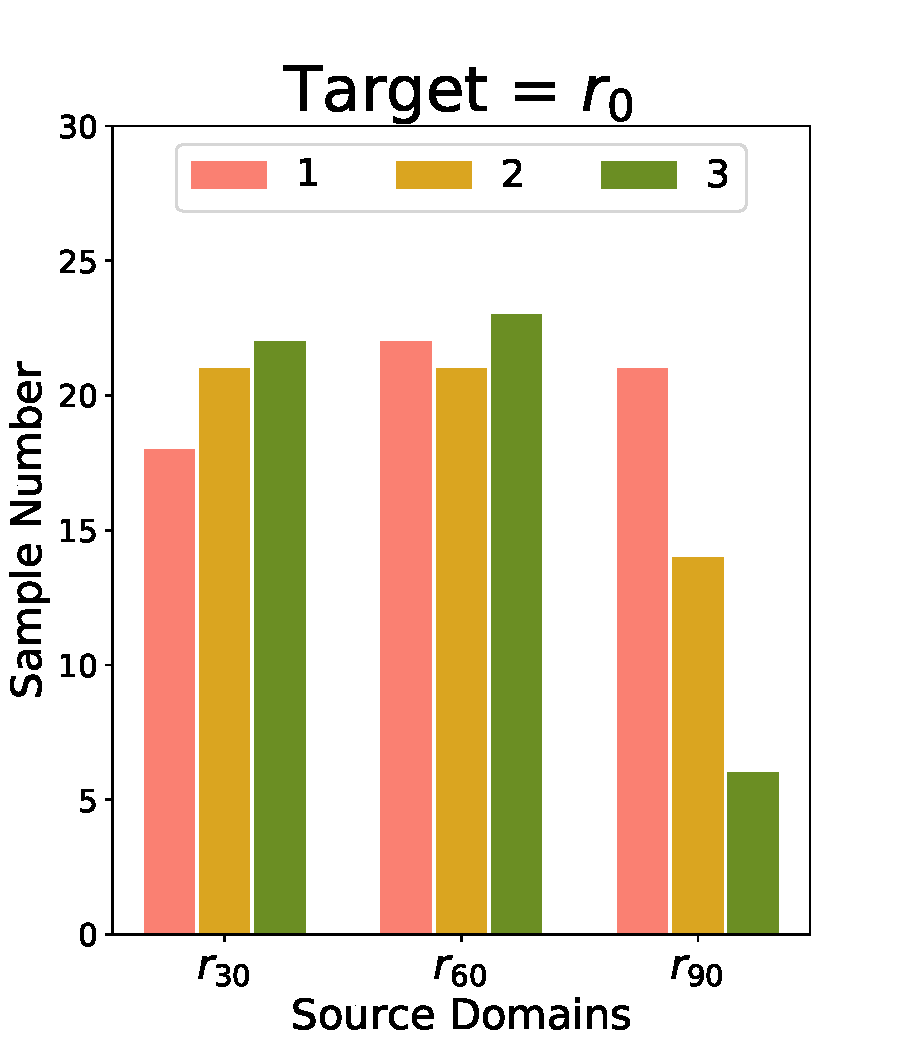
\includegraphics[width=0.2\linewidth]{figures/rmnist_imbalance/num_distribution/rmnist_imbalancerotation_0.pdf}\label{subfig:rmnist_results_0}}
%   \subfloat[$r_{30}$] 
    {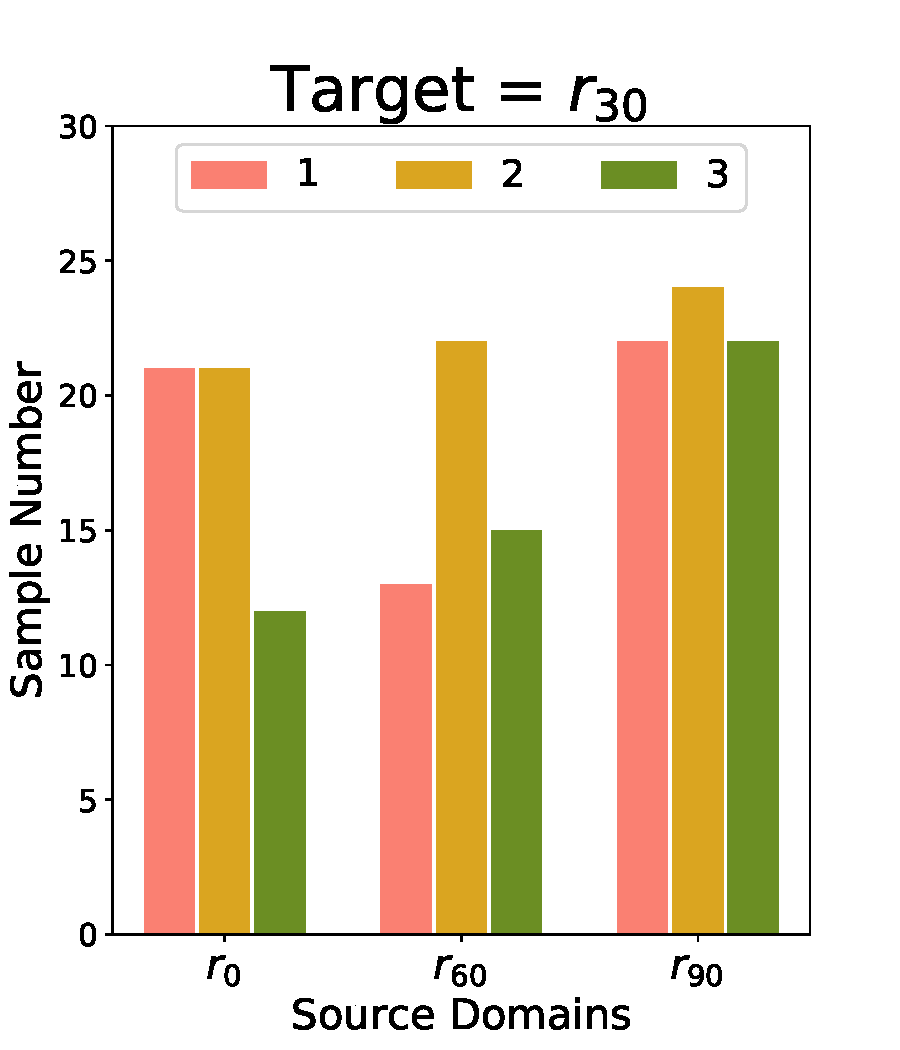
\includegraphics[width=0.2\linewidth]{figures/rmnist_imbalance/num_distribution/rmnist_imbalancerotation_30.pdf}\label{subfig:rmnist_results_30}}
%   \quad 
%   \subfloat[$r_{60}$]
    {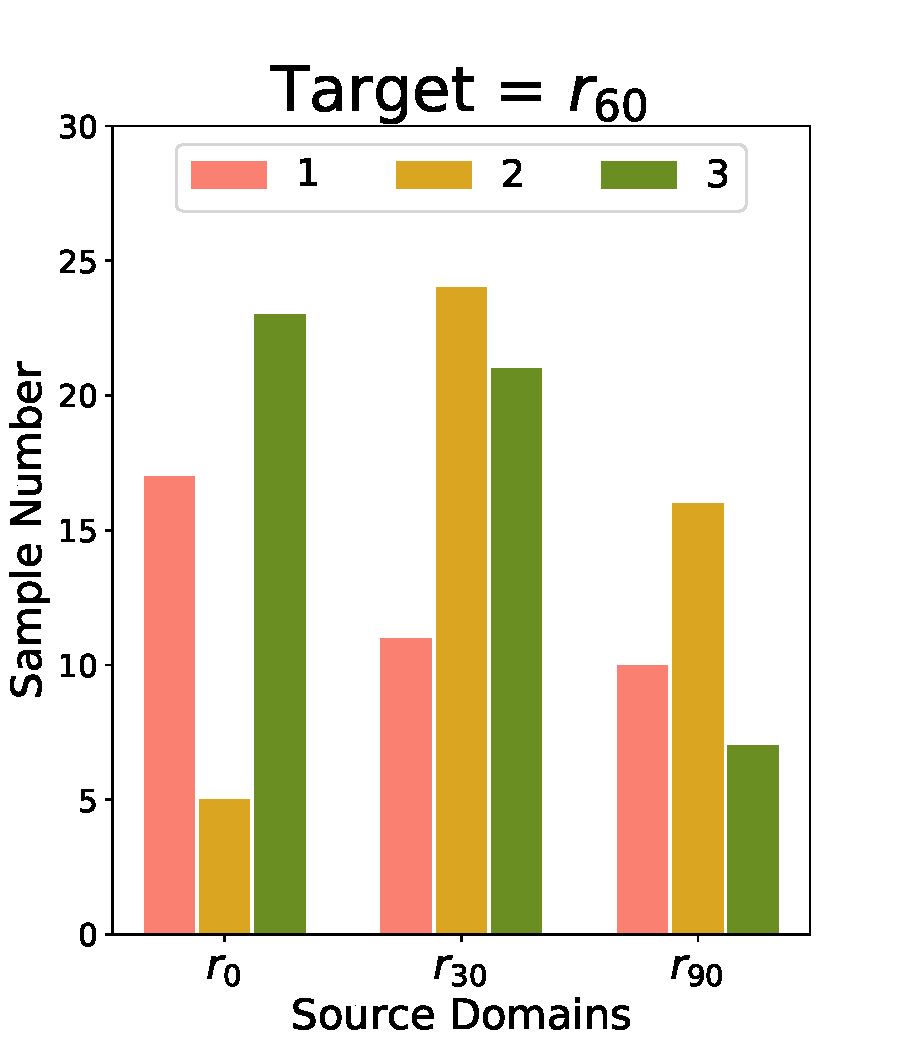
\includegraphics[width=0.2\linewidth]{figures/rmnist_imbalance/num_distribution/rmnist_imbalancerotation_60.pdf} \label{subfig:rmnist_results_60}}
%   \subfloat[$r_{90}$] 
    {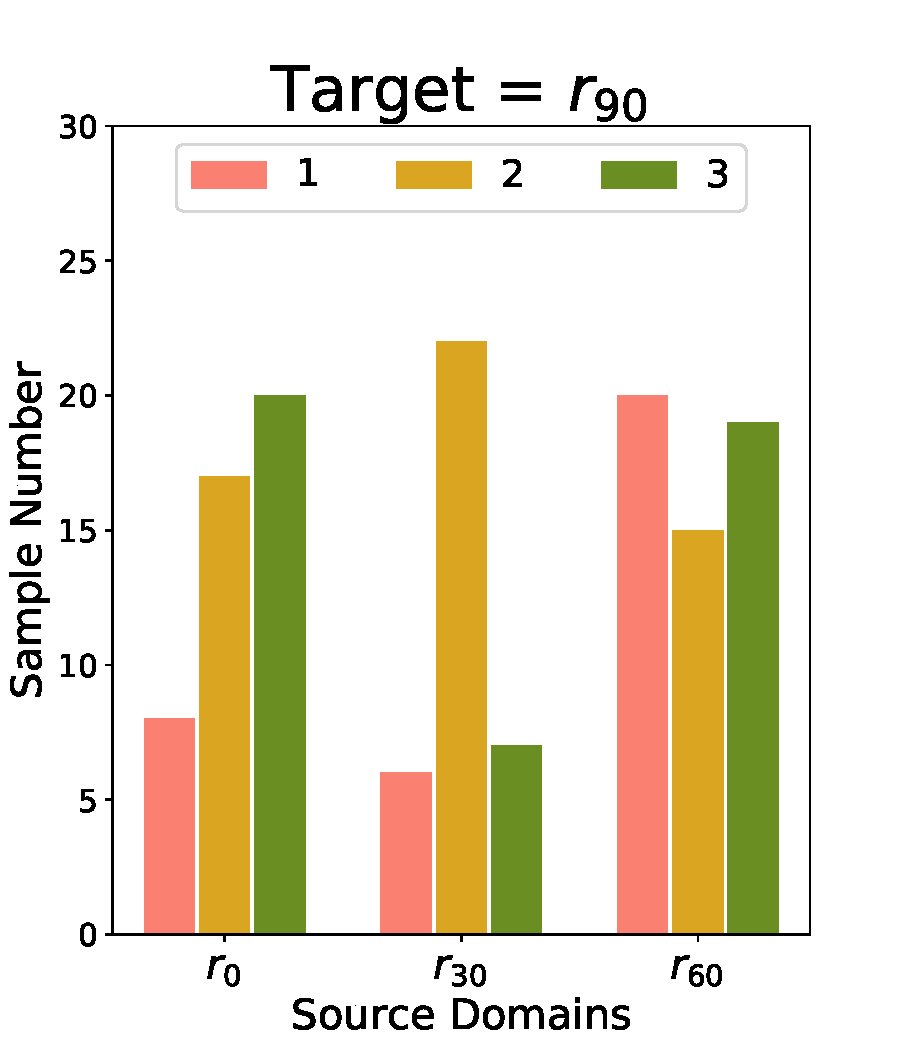
\includegraphics[width=0.2\linewidth]{figures/rmnist_imbalance/num_distribution/rmnist_imbalancerotation_90.pdf}\label{subfig:rmnist_results_90}}
  \caption{Visualization of random sample size for each class in source domains when a different domain serves as the target domain in the Rotated MNIST dataset. For each source domain, the number of samples for different classes are shown in different colors. There are cases when different classes have similar sample number, e.g., Class 1 and 2 of source domain $r_0$ when target domain is $r_{30}$, and also cases when different classes have quite different number of samples, e.g., in source domain $r_{90}$ when target domain is $r_{0}$.}
  \label{fig:rmnist_imbalance_distribution}
\end{figure*}

\begin{figure}%[h]
    \centering
    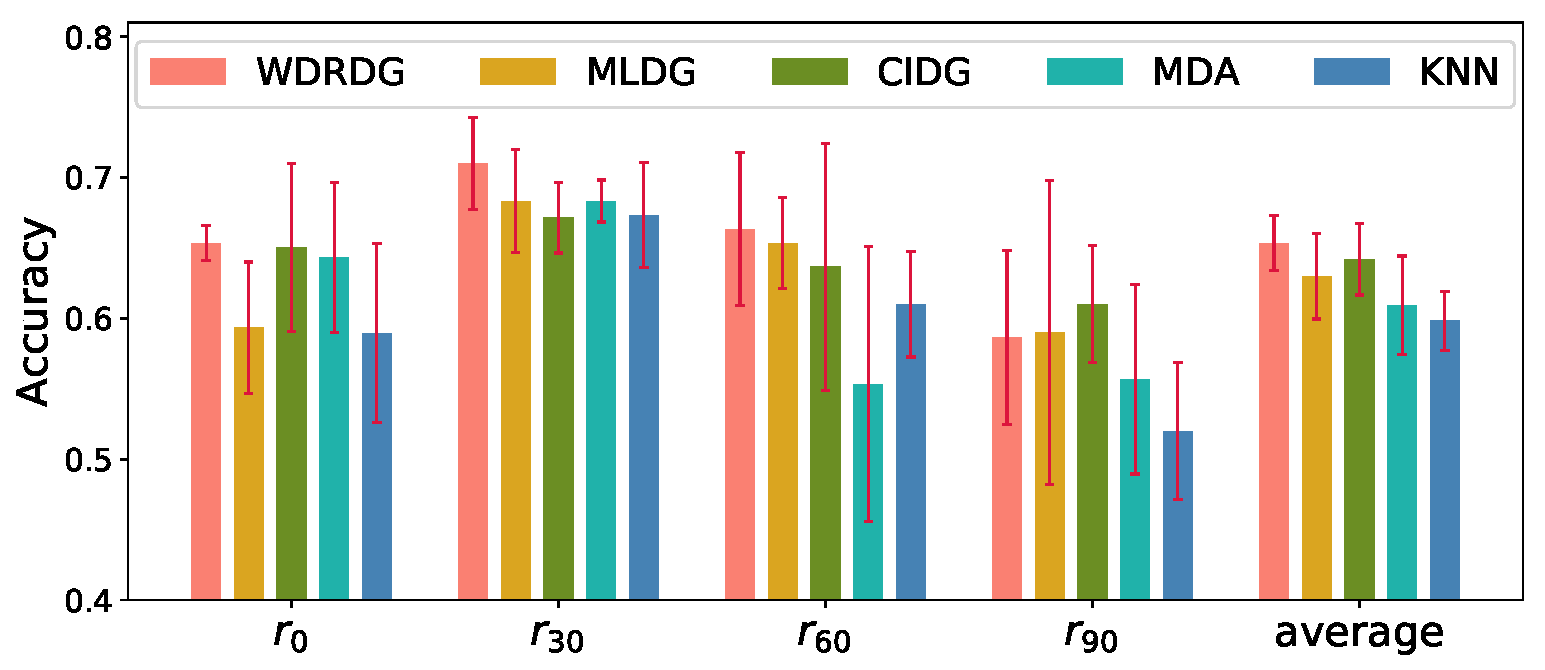
\includegraphics[scale=0.3]{figures/rmnist_imbalance/rmnist_imbalance_results.pdf}
    \caption{The performance of WDRDG and four compared methods on the Rotated MNIST dataset with different class prior distributions across source domains.  WDRDG outperforms other baselines by at least
$0.51\%$, $3.90\%$, $1.53\%$ when the target domain is $r_{0}$, $r_{30}$, $r_{60}$, respectively, and achieves similar accuracies with MLDG but with smaller deviation when the target domain is $r_{90}$.}
    \label{fig:rmnist_imbalance_results}
\end{figure}
In previous experiments, we actually assume the training sample size per class in the source domains are the same under the setting of no class prior distribution shift, i.e., the distribution of $P(Y)$ is the same across all source domains. 
To show the feasibility of extending our framework to scenarios with class prior distribution shift, we further conduct experiments when the categories in source domains are imbalanced, i.e., there are shifts among $P(Y)$ of different domains. 
% In a more general classification problem, to compensate for the possible class imbalance scenario, a series of class-weighting methods have been proposed to assign different weights to misclassifying samples from different classes \cite{zhou2005training,scott2012calibrated}.
% One of the most natural approaches is to incorporate the class prior distributions $\mathbb{P}(y=k)$ of each class into the risk function \cite{aurelio2019learning,xu2020class} as
% \begin{equation}
% \Psi\left(\phi; P_{1}, \ldots P_{K}\right)=\sum_{k=1}^{K} \mathbb{P}(y=k) \underset{\boldsymbol{x} \sim P_{k}}{\mathbb{E}}\left[1-\phi_{k}(\boldsymbol{x})\right].
% \label{eq:weighted_risk_function}
% \end{equation}
% The corresponding risk of the optimal classifier given $P_1, \ldots,P_K$ will become:
% \begin{equation}
%     \begin{aligned}
%     &\min_{\phi:\mathcal{X}\rightarrow \Delta_K}\Psi(\phi;,P_1,\ldots,P_K)\\
%     &= 1-\sum_{l=1}^n \max _{1 \leq k \leq K} \mathbb{P}(y=k) P_{k}(\boldsymbol{x}_l)
%     \end{aligned}
%     \label{eq:imbalance_obj}
% \end{equation}

We randomly sample the training sample size for each class from $[5,25)$ on the Rotated MNIST dataset here. The distribution of sample number for each class when each domain is chosen as the target domain is shown in Figure \ref{fig:rmnist_imbalance_distribution}.
There are cases when different classes have similar sample number, e.g., in source domain $r_{90}$ when the target domain is $r_{30}$, or in source domain $r_{60}$ when the target domain is $r_{0}$.  
In other source domains, different classes may have quite different number of samples, e.g., in source domain $r_{90}$ when target domain is $r_{0}$, or in source domain $r_{0}$ when target domain is $r_{60}$.
We compare our framework WDRDG with other methods, and the results are shown in Figure \ref{fig:rmnist_imbalance_results}.
When the target domain is $r_{90}$, our method achieves similar accuracies with MLDG but with smaller deviation, while in other cases WDRDG outperforms other baselines by at least
$0.51\%$, $3.90\%$, $1.53\%$ when the target domain is $r_{0}$, $r_{30}$, $r_{60}$, respectively. 
Our framework outperforms other methods on average with smaller standard deviation, which validates the generalization ability of our framework when the source domains have class prior distribution shift. 



\section{Conclusion}
In this research, we proposed a novel framework for domain generalization to enhance model robustness when labeled training data of source domains are limited.
We formulated the distributional shifts for each class with class-specific Wasserstein uncertainty sets and optimized the model over the worst-case distributions residing in the uncertainty sets via distributionally robust optimization. 
To reduce the difference between source and target domains, we proposed a test-time domain adaptation module through optimal transport to make adaptive inference for unseen target data. We found that our domain generalization framework with this adaptive inference module works better when target domains are more different compared with source domains. 
Experimental results on Rotated MNIST, PACS and VLCS datasets demonstrate that our proposed WDRDG framework could learn a robust model for unseen target domains based on limited source data, and we also showed that its advantage is more obvious in few-shot settings. 
To perfect this work in the future,  we would study the usage of class priors in constructing more realistic uncertainty sets, and explore measurable relationship among source domains to better leverage the source distributions to model possible target distributions. 



% % use section* for acknowledgment
\ifCLASSOPTIONcompsoc
  % The Computer Society usually uses the plural form
  \section*{Acknowledgments}
\else
  % regular IEEE prefers the singular form
  \section*{Acknowledgment}
  This study is supported in part by the Tsinghua SIGS Scientific Research Start-up Fund (Grant QD2021012C) and Natural Science Foundation of China (Grant 62001266).
\fi


% The authors would like to thank...
% This should be a simple paragraph before the References to thank those individuals and institutions who have supported your work on this article.




% Can use something like this to put references on a page
% by themselves when using endfloat and the captionsoff option.
\ifCLASSOPTIONcaptionsoff
  \newpage
\fi


% references section

% can use a bibliography generated by BibTeX as a .bbl file
% BibTeX documentation can be easily obtained at:
% http://mirror.ctan.org/biblio/bibtex/contrib/doc/
% The IEEEtran BibTeX style support page is at:
% http://www.michaelshell.org/tex/ieeetran/bibtex/
\bibliographystyle{IEEEtran}
% argument is your BibTeX string definitions and bibliography database(s)
\bibliography{references}
%
% <OR> manually copy in the resultant .bbl file
% set second argument of \begin to the number of references
% (used to reserve space for the reference number labels box)
% \begin{thebibliography}{1}

% \bibitem{IEEEhowto:kopka}
% H.~Kopka and P.~W. Daly, \emph{A Guide to \LaTeX}, 3rd~ed.\hskip 1em plus
%   0.5em minus 0.4em\relax Harlow, England: Addison-Wesley, 1999.

% \end{thebibliography}

% biography section
% 
% If you have an EPS/PDF photo (graphicx package needed) extra braces are
% needed around the contents of the optional argument to biography to prevent
% the LaTeX parser from getting confused when it sees the complicated
% \includegraphics command within an optional argument. (You could create
% your own custom macro containing the \includegraphics command to make things
% simpler here.)
%\begin{IEEEbiography}[{\includegraphics[width=1in,height=1.25in,clip,keepaspectratio]{mshell}}]{Michael Shell}
% or if you just want to reserve a space for a photo:









% \begin{IEEEbiography}[{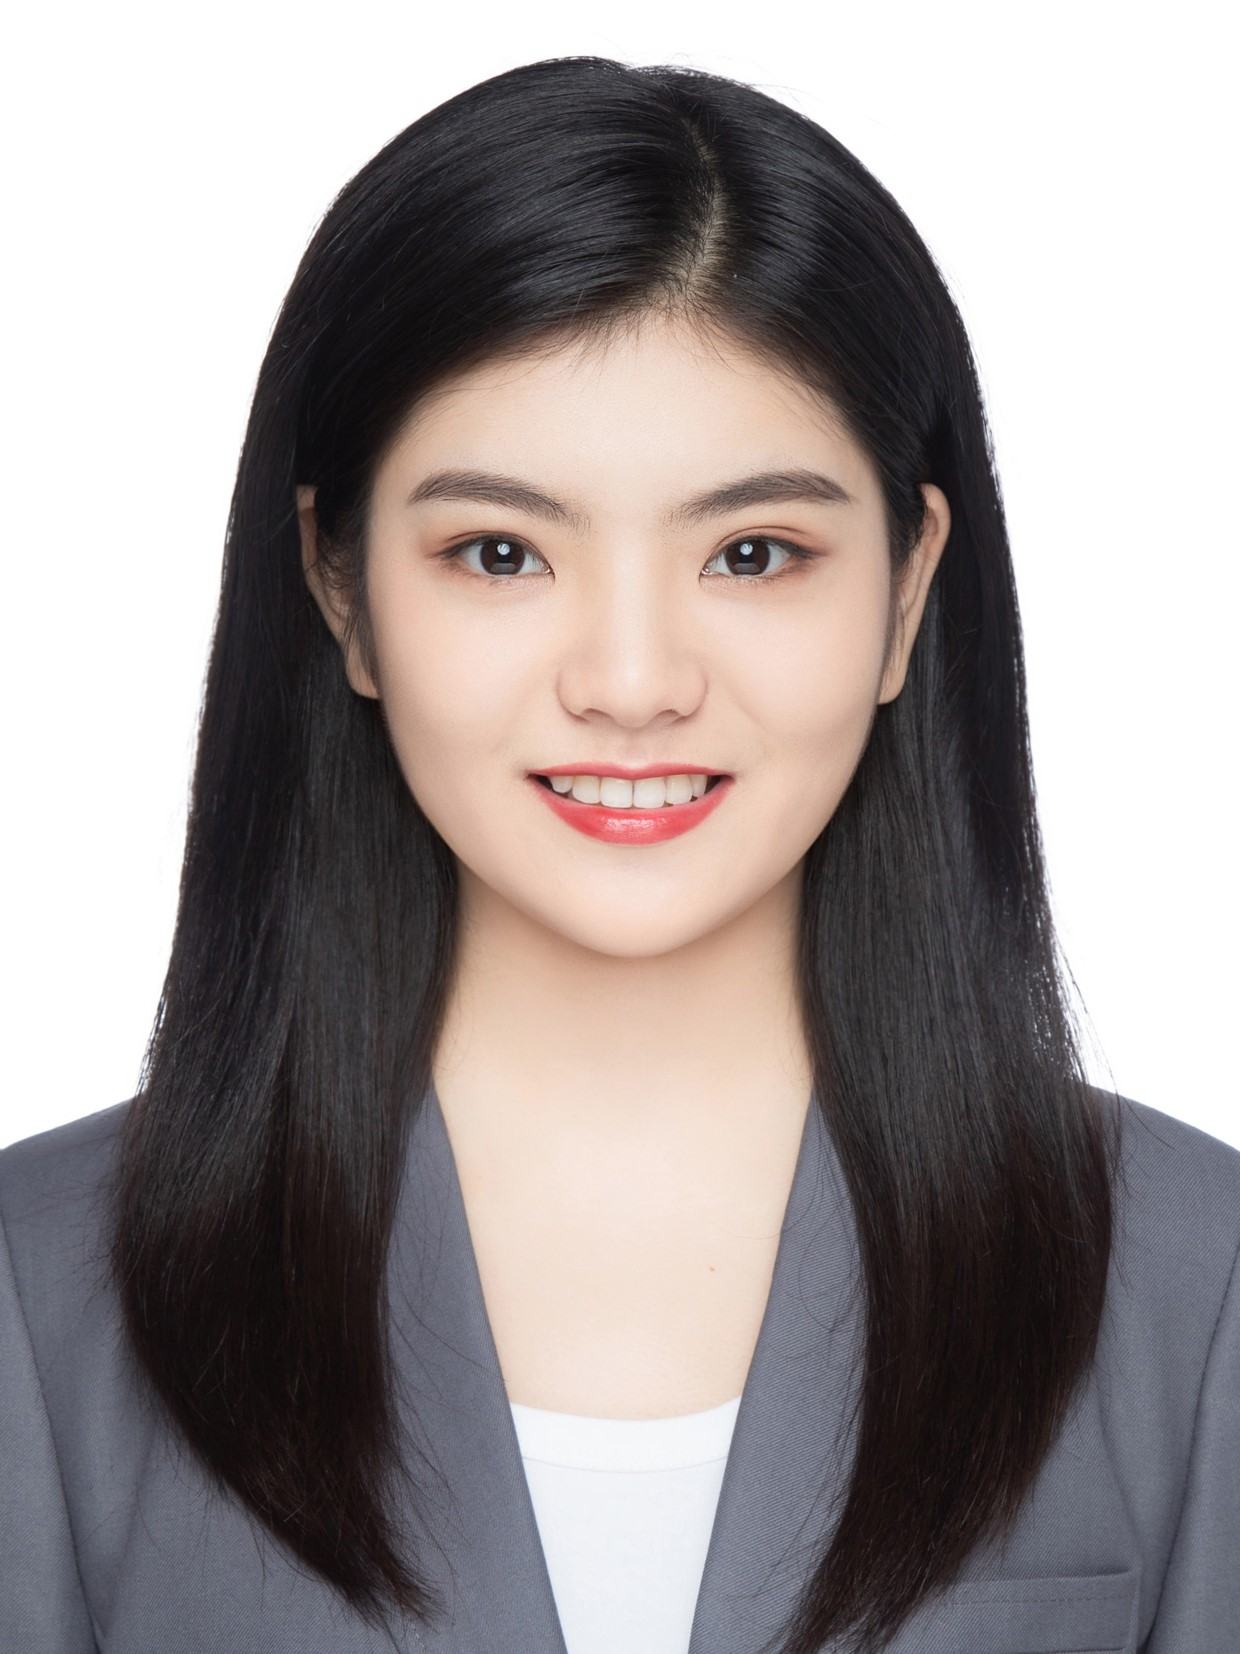
\includegraphics[width=1in,height=1.25in,clip,keepaspectratio]{biography/jinggewang.jpg}}]{Jingge Wang} (Student Member, IEEE) received her B.E. degree in Automation in 2019 from the School of Artificial Intelligence and Automation, Huazhong University of Science and Technology, Hubei, China, and her M.S. degree from Tsinghua-Berkeley Shenzhen Institute, Tsinghua University in 2022. She is currently working towards the Ph.D. degree 
% at Tsinghua-Berkeley Shenzhen Institute, Tsinghua University, China. Her research interests include transfer learning and domain generalization with multiple domains with small data.
% \end{IEEEbiography}



% \begin{IEEEbiography}[{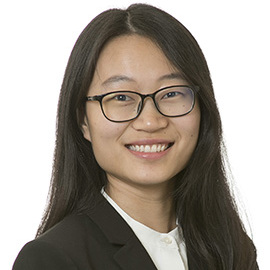
\includegraphics[width=1in,height=1.25in,clip,keepaspectratio]{biography/liyan.jpg}}]{Liyan Xie} received the B.Sc. degree in statistics from the University of Science and Technology of China in 2016, and her Ph.D. degree in Industrial Engineering from Georgia Institute of Technology in 2021. Since 2021, She has been an assistant professor in School of Data Science at The Chinese University of Hong Kong, Shenzhen. Her research interests are the intersection between statistics and optimization, with a primary focus on sequential change detection, robust hypothesis testing, transfer learning, and their applications in sensor networks and healthcare. She was awarded the finalist of the INFORMS QSR Student Paper Competition and Runner-up for the INFORMS Computing Society Student Paper Prize in 2019.
% \end{IEEEbiography}


% \begin{IEEEbiography}[{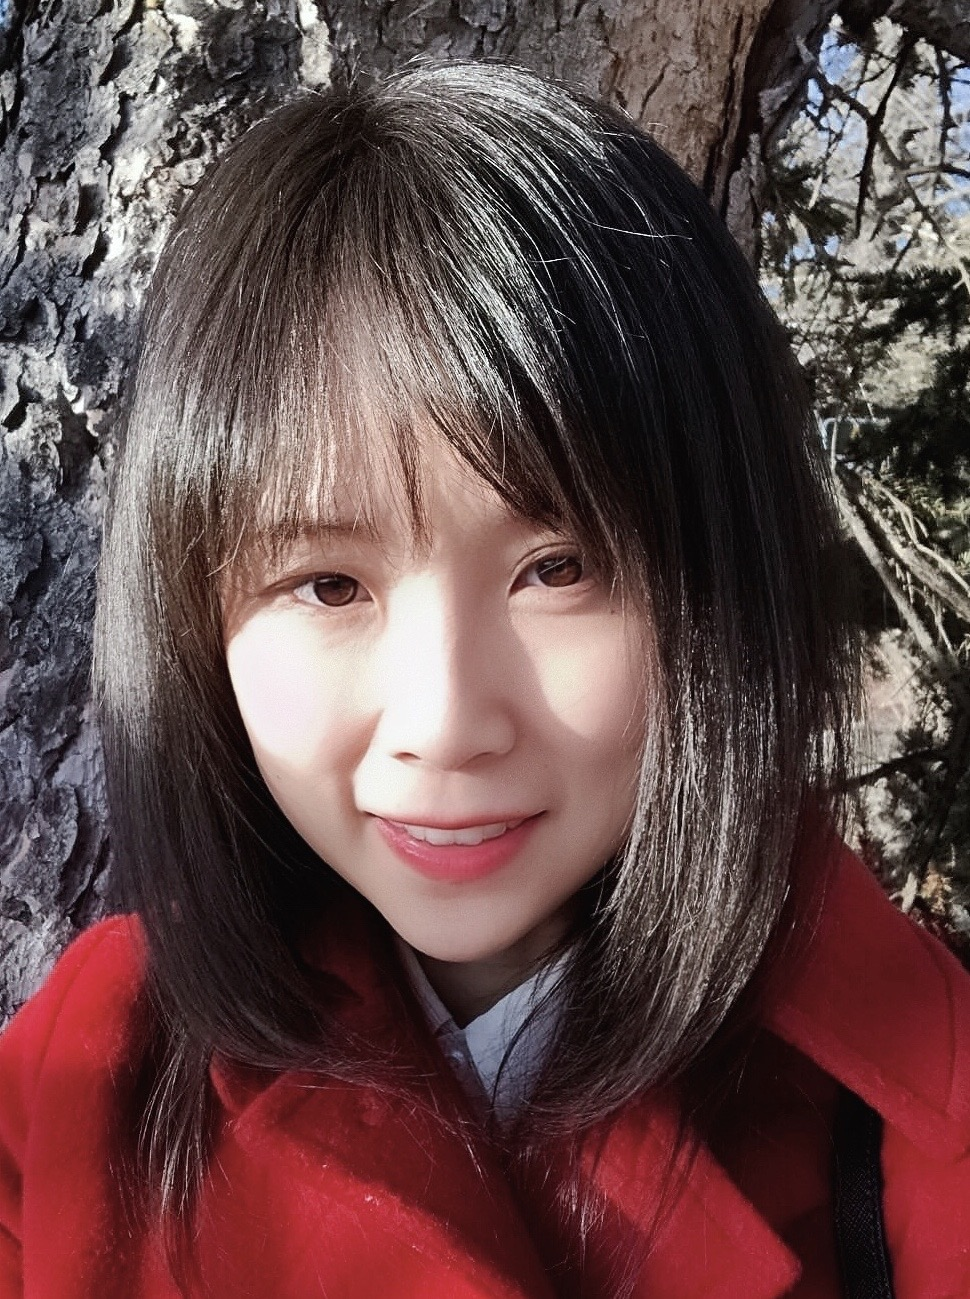
\includegraphics[width=1in,height=1.25in,clip,keepaspectratio]{biography/yaoxie.jpg}}]{Yao Xie}
% is an Associate Professor and Harold R. and Mary Anne Nash Early Career Professor at Georgia Institute of Technology in the H. Milton Stewart School of Industrial and Systems Engineering, and an Associate Director of the Machine Learning Center. She received her Ph.D. in Electrical Engineering (minor in Mathematics) from Stanford University and was a Research Scientist at Duke University. Her research areas are statistics (particularly change-point detection and spatio-temporal data modeling), machine learning, and signal processing, providing the theoretical foundation and developing computationally efficient and statistically powerful algorithms for engineering problems. She received the National Science Foundation (NSF) CAREER Award in 2017. She is currently an Associate Editor for IEEE Transactions on Information Theory, IEEE Transactions on Signal Processing, Sequential Analysis: Design Methods and Applications, INFORMS Journal on Data Science, and serves on the Editorial Board of Journal of Machine Learning Research, and an Area Chair of NeurIPS in 2021 and 2022.
% \end{IEEEbiography}



% \begin{IEEEbiography}[{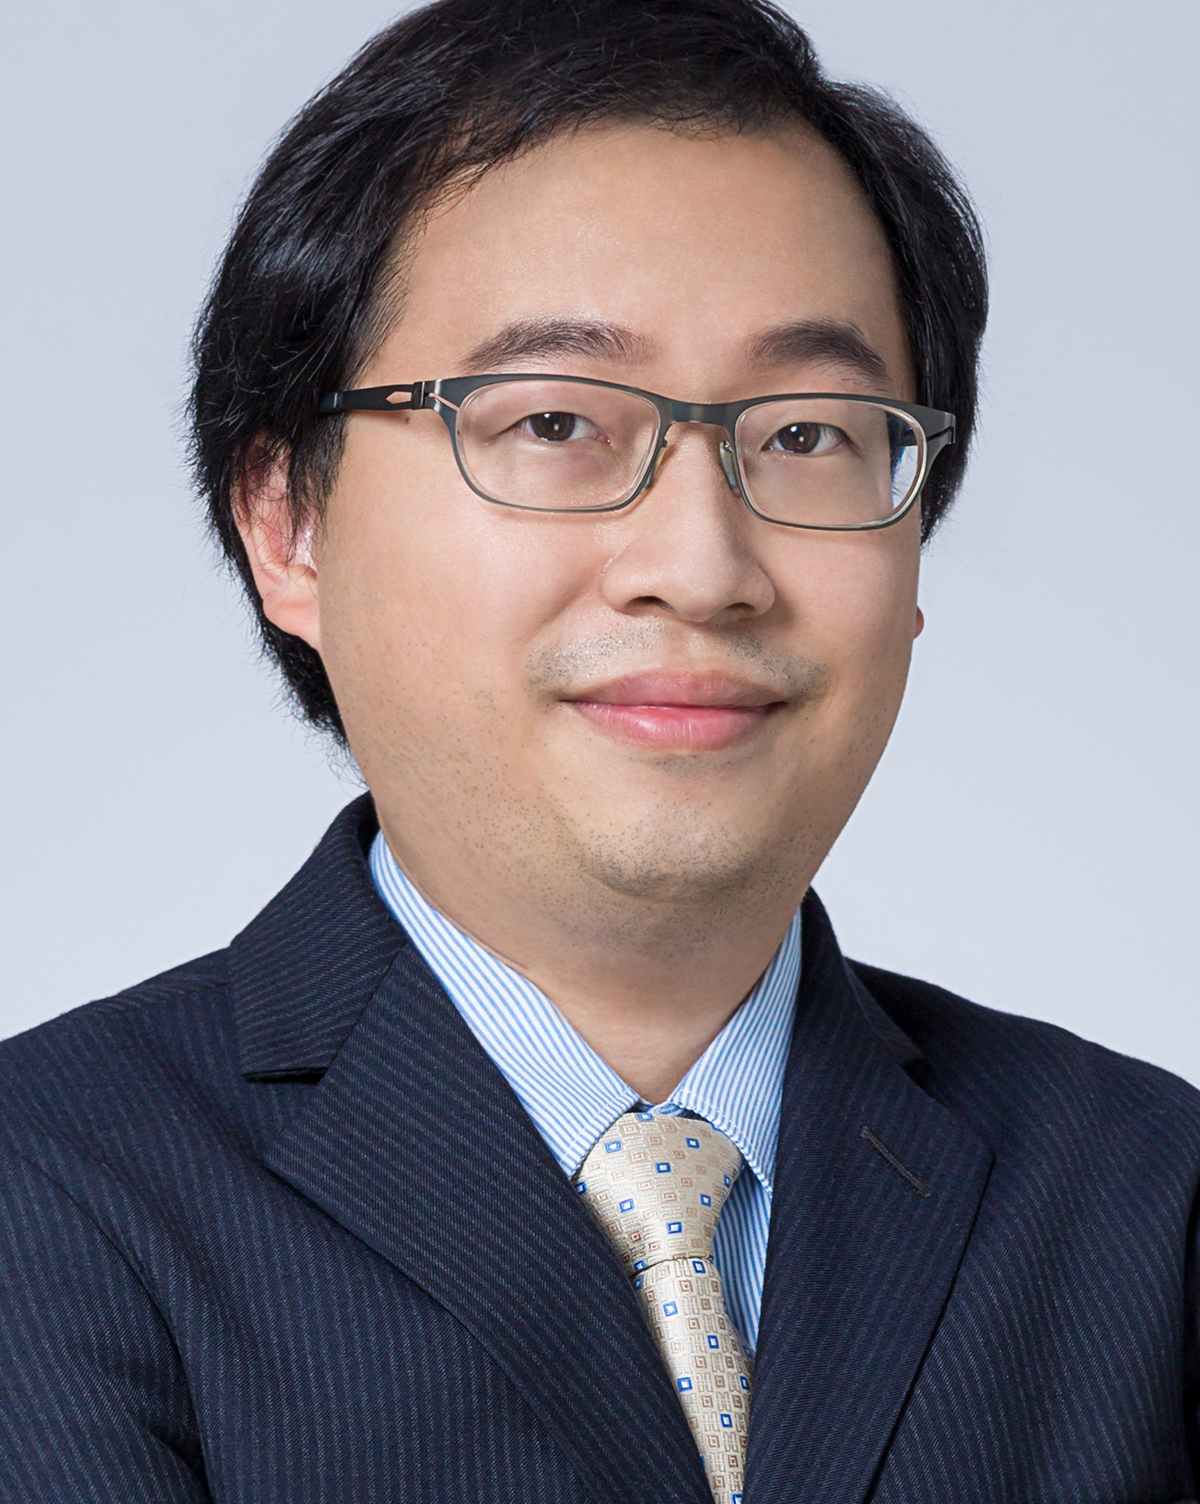
\includegraphics[width=1in,height=1.25in,clip,keepaspectratio]{biography/shaolunhuang.png}}]{Shao-Lun Huang}
% (Member, IEEE) received the B.S. degree with honor in 2008 from the Department of Electronic Engineering, National Taiwan University, Taiwan, and the M.S. and Ph.D. degree in 2010 and 2013 from the Department of Electronic Engineering and Computer Sciences, Massachusetts Institute of Technology. From 2013 to 2016, he was working as a postdoctoral researcher jointly in the Department of Electrical Engineering at the National Taiwan University and the Department of Electrical Engineering and Computer Science at the Massachusetts Institute of Technology. Since 2016, he has joined Tsinghua-Berkeley Shenzhen Institute, where he is currently an associate professor. His research interests include information theory, communication theory, machine learning, and social networks.
% \end{IEEEbiography}


% \begin{IEEEbiography}[{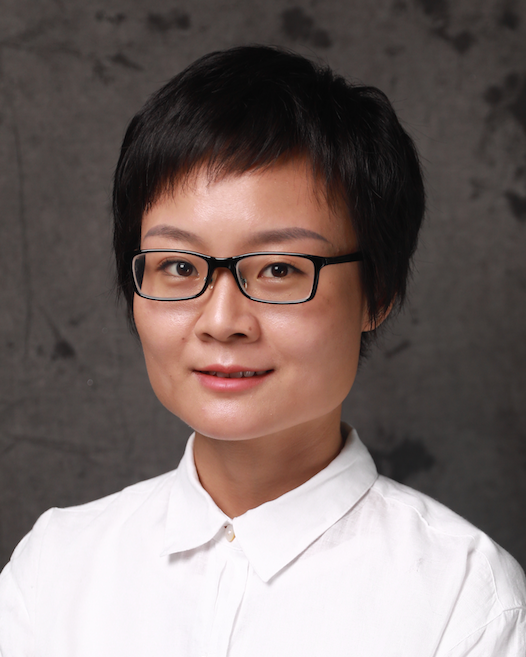
\includegraphics[width=1in,height=1.25in,clip,keepaspectratio]{biography/yangli.png}}]{Yang Li}
%  (Member, IEEE) received her B.A. degree in computer science and mathematics from Smith College in 2011, and her Ph.D. degree in computer science from Stanford University in 2017. She had been a postdoctoral fellow at Tsinghua-Berkeley Shenzhen Institute, China from 2017-2019. Since 2019, she has been an assistant professor at the Data Science and Information Technology Research Center of Tsinghua-Berkeley Shenzhen Institute.  Her research interests include transfer learning, representation learning with multiple tasks and domains, spatial data analysis and geometric algorithms.
% \end{IEEEbiography}



% insert where needed to balance the two columns on the last page with
% biographies
%\newpage


% You can push biographies down or up by placing
% a \vfill before or after them. The appropriate
% use of \vfill depends on what kind of text is
% on the last page and whether or not the columns
% are being equalized.

%\vfill

% Can be used to pull up biographies so that the bottom of the last one
% is flush with the other column.
%\enlargethispage{-5in}



% that's all folks
\end{document}


